\documentclass[twoside]{article}

% Packages required by doxygen
\usepackage{fixltx2e}
\usepackage{calc}
\usepackage{doxygen}
\usepackage[export]{adjustbox} % also loads graphicx
\usepackage{graphicx}
\usepackage[utf8]{inputenc}
\usepackage{makeidx}
\usepackage{multicol}
\usepackage{multirow}
\PassOptionsToPackage{warn}{textcomp}
\usepackage{textcomp}
\usepackage[nointegrals]{wasysym}
\usepackage[table]{xcolor}

% Font selection
\usepackage[T1]{fontenc}
\usepackage[scaled=.90]{helvet}
\usepackage{courier}
\usepackage{amssymb}
\usepackage{sectsty}
\renewcommand{\familydefault}{\sfdefault}
\allsectionsfont{%
  \fontseries{bc}\selectfont%
  \color{darkgray}%
}
\renewcommand{\DoxyLabelFont}{%
  \fontseries{bc}\selectfont%
  \color{darkgray}%
}
\newcommand{\+}{\discretionary{\mbox{\scriptsize$\hookleftarrow$}}{}{}}

% Page & text layout
\usepackage{geometry}
\geometry{%
  letterpaper,%
  top=2.5cm,%
  bottom=2.5cm,%
  left=2.5cm,%
  right=2.5cm%
}
\tolerance=750
\hfuzz=15pt
\hbadness=750
\setlength{\emergencystretch}{15pt}
\setlength{\parindent}{0cm}
\setlength{\parskip}{3ex plus 2ex minus 2ex}
\makeatletter
\renewcommand{\paragraph}{%
  \@startsection{paragraph}{4}{0ex}{-1.0ex}{1.0ex}{%
    \normalfont\normalsize\bfseries\SS@parafont%
  }%
}
\renewcommand{\subparagraph}{%
  \@startsection{subparagraph}{5}{0ex}{-1.0ex}{1.0ex}{%
    \normalfont\normalsize\bfseries\SS@subparafont%
  }%
}
\makeatother

% Headers & footers
\usepackage{fancyhdr}
\pagestyle{fancyplain}
\fancyhead[LE]{\fancyplain{}{\bfseries\thepage}}
\fancyhead[CE]{\fancyplain{}{}}
\fancyhead[RE]{\fancyplain{}{\bfseries\leftmark}}
\fancyhead[LO]{\fancyplain{}{\bfseries\rightmark}}
\fancyhead[CO]{\fancyplain{}{}}
\fancyhead[RO]{\fancyplain{}{\bfseries\thepage}}
\fancyfoot[LE]{\fancyplain{}{}}
\fancyfoot[CE]{\fancyplain{}{}}
\fancyfoot[RE]{\fancyplain{}{\bfseries\scriptsize Generated by Doxygen }}
\fancyfoot[LO]{\fancyplain{}{\bfseries\scriptsize Generated by Doxygen }}
\fancyfoot[CO]{\fancyplain{}{}}
\fancyfoot[RO]{\fancyplain{}{}}
\renewcommand{\footrulewidth}{0.4pt}
\renewcommand{\sectionmark}[1]{%
  \markright{\thesection\ #1}%
}

% Indices & bibliography
\usepackage{natbib}
\usepackage[titles]{tocloft}
\setcounter{tocdepth}{3}
\setcounter{secnumdepth}{5}
\makeindex

% Hyperlinks (required, but should be loaded last)
\usepackage{ifpdf}
\ifpdf
  \usepackage[pdftex,pagebackref=true]{hyperref}
\else
  \usepackage[ps2pdf,pagebackref=true]{hyperref}
\fi
\hypersetup{%
  colorlinks=true,%
  linkcolor=blue,%
  citecolor=blue,%
  unicode%
}

% Custom commands
\newcommand{\clearemptydoublepage}{%
  \newpage{\pagestyle{empty}\cleardoublepage}%
}

\usepackage{caption}
\captionsetup{labelsep=space,justification=centering,font={bf},singlelinecheck=off,skip=4pt,position=top}

%===== C O N T E N T S =====

\begin{document}

% Titlepage & ToC
\hypersetup{pageanchor=false,
             bookmarksnumbered=true,
             pdfencoding=unicode
            }
\pagenumbering{alph}
\begin{titlepage}
\vspace*{7cm}
\begin{center}%
{\Large 9228B Tower Takeover Code \\[1ex]\large 2.\+1.\+4 }\\
\vspace*{1cm}
{\large Generated by Doxygen 1.8.14}\\
\end{center}
\end{titlepage}
\pagenumbering{roman}
\tableofcontents
\pagenumbering{arabic}
\hypersetup{pageanchor=true}

%--- Begin generated contents ---
\section{File Index}
\doxysection{File List}
Here is a list of all files with brief descriptions\+:\begin{DoxyCompactList}
\item\contentsline{section}{include/\mbox{\hyperlink{auton_8h}{auton.\+h}} }{\pageref{auton_8h}}{}
\item\contentsline{section}{include/\mbox{\hyperlink{controller_8h}{controller.\+h}} }{\pageref{controller_8h}}{}
\item\contentsline{section}{include/\mbox{\hyperlink{declarations_8h}{declarations.\+h}} }{\pageref{declarations_8h}}{}
\item\contentsline{section}{include/\mbox{\hyperlink{drive_8h}{drive.\+h}} }{\pageref{drive_8h}}{}
\item\contentsline{section}{include/\mbox{\hyperlink{init_8h}{init.\+h}} }{\pageref{init_8h}}{}
\item\contentsline{section}{include/\mbox{\hyperlink{vex_8h}{vex.\+h}} }{\pageref{vex_8h}}{}
\item\contentsline{section}{src/\mbox{\hyperlink{auton_8cpp}{auton.\+cpp}} }{\pageref{auton_8cpp}}{}
\item\contentsline{section}{src/\mbox{\hyperlink{controller_8cpp}{controller.\+cpp}} }{\pageref{controller_8cpp}}{}
\item\contentsline{section}{src/\mbox{\hyperlink{drive_8cpp}{drive.\+cpp}} }{\pageref{drive_8cpp}}{}
\item\contentsline{section}{src/\mbox{\hyperlink{init_8cpp}{init.\+cpp}} }{\pageref{init_8cpp}}{}
\item\contentsline{section}{src/\mbox{\hyperlink{main_8cpp}{main.\+cpp}} }{\pageref{main_8cpp}}{}
\end{DoxyCompactList}

\section{File Documentation}
\hypertarget{auton_8h}{}\subsection{include/auton.h File Reference}
\label{auton_8h}\index{include/auton.\+h@{include/auton.\+h}}
\subsubsection*{Enumerations}
\begin{DoxyCompactItemize}
\item 
enum \mbox{\hyperlink{auton_8h_a78abb31bad0fd1834c54a3ca6f8daab5_a78abb31bad0fd1834c54a3ca6f8daab5}{Color}} \+: bool \{ \mbox{\hyperlink{auton_8h_a78abb31bad0fd1834c54a3ca6f8daab5_a78abb31bad0fd1834c54a3ca6f8daab5a1b3e1ee9bff86431dea6b181365ba65f}{Color\+::\+B\+L\+UE}} = false, 
\mbox{\hyperlink{auton_8h_a78abb31bad0fd1834c54a3ca6f8daab5_a78abb31bad0fd1834c54a3ca6f8daab5aa2d9547b5d3dd9f05984475f7c926da0}{Color\+::\+R\+ED}} = true
 \}
\item 
enum \mbox{\hyperlink{auton_8h_a702107095bd059695d57318e7338a4a7_a702107095bd059695d57318e7338a4a7}{Side}} \+: bool \{ \mbox{\hyperlink{auton_8h_a702107095bd059695d57318e7338a4a7_a702107095bd059695d57318e7338a4a7a684d325a7303f52e64011467ff5c5758}{Side\+::\+L\+E\+FT}} = false, 
\mbox{\hyperlink{auton_8h_a702107095bd059695d57318e7338a4a7_a702107095bd059695d57318e7338a4a7a21507b40c80068eda19865706fdc2403}{Side\+::\+R\+I\+G\+HT}} = true
 \}
\end{DoxyCompactItemize}
\subsubsection*{Functions}
\begin{DoxyCompactItemize}
\item 
bool \mbox{\hyperlink{auton_8h_ad35d3bfeb2cba05d92e52e9a6fd7886f_ad35d3bfeb2cba05d92e52e9a6fd7886f}{move\+Forward}} (double inches, double speed, bool blocking)
\item 
bool \mbox{\hyperlink{auton_8h_a29cfffc5489f3d18bde443edb5b14e33_a29cfffc5489f3d18bde443edb5b14e33}{pivot\+Clockwise}} (float degrees, bool blocking)
\item 
bool \mbox{\hyperlink{auton_8h_a8969639a29fd3bc748acbc0797955fb9_a8969639a29fd3bc748acbc0797955fb9}{pivot\+Counter\+Clockwise}} (float degrees, bool blocking)
\item 
void \mbox{\hyperlink{auton_8h_a9c7e58a3b4bb5cdd30a6b3ed32e8f962_a9c7e58a3b4bb5cdd30a6b3ed32e8f962}{auton}} (\mbox{\hyperlink{auton_8h_a702107095bd059695d57318e7338a4a7_a702107095bd059695d57318e7338a4a7}{Side}} side, \mbox{\hyperlink{auton_8h_a78abb31bad0fd1834c54a3ca6f8daab5_a78abb31bad0fd1834c54a3ca6f8daab5}{Color}} color)
\begin{DoxyCompactList}\small\item\em the autonomous switcher \end{DoxyCompactList}\item 
bool \mbox{\hyperlink{auton_8h_abba3fa3f69d7ee97541aa1169ee13cee_abba3fa3f69d7ee97541aa1169ee13cee}{auton\+Start}} ()
\item 
void \mbox{\hyperlink{auton_8h_a5bb01d00c76862cb15431efd4090bee9_a5bb01d00c76862cb15431efd4090bee9}{auton\+Blue\+Left}} ()
\item 
void \mbox{\hyperlink{auton_8h_ab9984e9a12048995fb71a06a1c94fd31_ab9984e9a12048995fb71a06a1c94fd31}{auton\+Blue\+Right}} ()
\item 
void \mbox{\hyperlink{auton_8h_aae46c4423bc7ed2947e82c4c5dd7f469_aae46c4423bc7ed2947e82c4c5dd7f469}{auton\+Red\+Left}} ()
\item 
void \mbox{\hyperlink{auton_8h_aaf3b274e9144b7072829ca58203492a6_aaf3b274e9144b7072829ca58203492a6}{auton\+Red\+Right}} ()
\item 
void \mbox{\hyperlink{auton_8h_af9785dd062d532b02b46976d0b757c9e_af9785dd062d532b02b46976d0b757c9e}{bad\+Auton}} (\mbox{\hyperlink{auton_8h_a702107095bd059695d57318e7338a4a7_a702107095bd059695d57318e7338a4a7}{Side}} side, \mbox{\hyperlink{auton_8h_a78abb31bad0fd1834c54a3ca6f8daab5_a78abb31bad0fd1834c54a3ca6f8daab5}{Color}} color)
\item 
void \mbox{\hyperlink{auton_8h_a36ea406b10e4d9a8d67e2fb46e8e7185_a36ea406b10e4d9a8d67e2fb46e8e7185}{bad\+Auton\+Blue\+Left}} ()
\item 
void \mbox{\hyperlink{auton_8h_ac18b0a3ac7170bb6dfa70ba82f176f5b_ac18b0a3ac7170bb6dfa70ba82f176f5b}{bad\+Auton\+Blue\+Right}} ()
\item 
void \mbox{\hyperlink{auton_8h_a6a7a31dcb74151b019518167ccb145ae_a6a7a31dcb74151b019518167ccb145ae}{bad\+Auton\+Red\+Left}} ()
\item 
void \mbox{\hyperlink{auton_8h_a84717ac55c83eb1faa4c1952a570950a_a84717ac55c83eb1faa4c1952a570950a}{bad\+Auton\+Red\+Right}} ()
\end{DoxyCompactItemize}


\subsubsection{Enumeration Type Documentation}
\mbox{\Hypertarget{auton_8h_a78abb31bad0fd1834c54a3ca6f8daab5_a78abb31bad0fd1834c54a3ca6f8daab5}\label{auton_8h_a78abb31bad0fd1834c54a3ca6f8daab5_a78abb31bad0fd1834c54a3ca6f8daab5}} 
\index{auton.\+h@{auton.\+h}!Color@{Color}}
\index{Color@{Color}!auton.\+h@{auton.\+h}}
\paragraph{\texorpdfstring{Color}{Color}}
{\footnotesize\ttfamily enum \mbox{\hyperlink{auton_8h_a78abb31bad0fd1834c54a3ca6f8daab5_a78abb31bad0fd1834c54a3ca6f8daab5}{Color}} \+: bool\hspace{0.3cm}{\ttfamily [strong]}}

Declares the possible autonomous colors for the autonomous switcher \begin{DoxyAuthor}{Author}
Michael Baraty 
\end{DoxyAuthor}
\begin{DoxyDate}{Date}
11/9/2019 
\end{DoxyDate}
\begin{DoxyEnumFields}{Enumerator}
\raisebox{\heightof{T}}[0pt][0pt]{\index{B\+L\+UE@{B\+L\+UE}!auton.\+h@{auton.\+h}}\index{auton.\+h@{auton.\+h}!B\+L\+UE@{B\+L\+UE}}}\mbox{\Hypertarget{auton_8h_a78abb31bad0fd1834c54a3ca6f8daab5_a78abb31bad0fd1834c54a3ca6f8daab5a1b3e1ee9bff86431dea6b181365ba65f}\label{auton_8h_a78abb31bad0fd1834c54a3ca6f8daab5_a78abb31bad0fd1834c54a3ca6f8daab5a1b3e1ee9bff86431dea6b181365ba65f}} 
B\+L\+UE&\\
\hline

\raisebox{\heightof{T}}[0pt][0pt]{\index{R\+ED@{R\+ED}!auton.\+h@{auton.\+h}}\index{auton.\+h@{auton.\+h}!R\+ED@{R\+ED}}}\mbox{\Hypertarget{auton_8h_a78abb31bad0fd1834c54a3ca6f8daab5_a78abb31bad0fd1834c54a3ca6f8daab5aa2d9547b5d3dd9f05984475f7c926da0}\label{auton_8h_a78abb31bad0fd1834c54a3ca6f8daab5_a78abb31bad0fd1834c54a3ca6f8daab5aa2d9547b5d3dd9f05984475f7c926da0}} 
R\+ED&\\
\hline

\end{DoxyEnumFields}


Definition at line \mbox{\hyperlink{auton_8h_source_l00038}{38}} of file \mbox{\hyperlink{auton_8h_source}{auton.\+h}}.


\begin{DoxyCode}
00038                  : \textcolor{keywordtype}{bool} \{
00039   \mbox{\hyperlink{auton_8h_a78abb31bad0fd1834c54a3ca6f8daab5_a78abb31bad0fd1834c54a3ca6f8daab5a1b3e1ee9bff86431dea6b181365ba65f}{BLUE}} = \textcolor{keyword}{false},
00040   \mbox{\hyperlink{auton_8h_a78abb31bad0fd1834c54a3ca6f8daab5_a78abb31bad0fd1834c54a3ca6f8daab5aa2d9547b5d3dd9f05984475f7c926da0}{RED}} = \textcolor{keyword}{true}
00041 \};
\end{DoxyCode}
\mbox{\Hypertarget{auton_8h_a702107095bd059695d57318e7338a4a7_a702107095bd059695d57318e7338a4a7}\label{auton_8h_a702107095bd059695d57318e7338a4a7_a702107095bd059695d57318e7338a4a7}} 
\index{auton.\+h@{auton.\+h}!Side@{Side}}
\index{Side@{Side}!auton.\+h@{auton.\+h}}
\paragraph{\texorpdfstring{Side}{Side}}
{\footnotesize\ttfamily enum \mbox{\hyperlink{auton_8h_a702107095bd059695d57318e7338a4a7_a702107095bd059695d57318e7338a4a7}{Side}} \+: bool\hspace{0.3cm}{\ttfamily [strong]}}

Declares the possible autonomous starting side for the autonomous switcher \begin{DoxyAuthor}{Author}
Michael Baraty 
\end{DoxyAuthor}
\begin{DoxyDate}{Date}
11/9/2019 
\end{DoxyDate}
\begin{DoxyEnumFields}{Enumerator}
\raisebox{\heightof{T}}[0pt][0pt]{\index{L\+E\+FT@{L\+E\+FT}!auton.\+h@{auton.\+h}}\index{auton.\+h@{auton.\+h}!L\+E\+FT@{L\+E\+FT}}}\mbox{\Hypertarget{auton_8h_a702107095bd059695d57318e7338a4a7_a702107095bd059695d57318e7338a4a7a684d325a7303f52e64011467ff5c5758}\label{auton_8h_a702107095bd059695d57318e7338a4a7_a702107095bd059695d57318e7338a4a7a684d325a7303f52e64011467ff5c5758}} 
L\+E\+FT&\\
\hline

\raisebox{\heightof{T}}[0pt][0pt]{\index{R\+I\+G\+HT@{R\+I\+G\+HT}!auton.\+h@{auton.\+h}}\index{auton.\+h@{auton.\+h}!R\+I\+G\+HT@{R\+I\+G\+HT}}}\mbox{\Hypertarget{auton_8h_a702107095bd059695d57318e7338a4a7_a702107095bd059695d57318e7338a4a7a21507b40c80068eda19865706fdc2403}\label{auton_8h_a702107095bd059695d57318e7338a4a7_a702107095bd059695d57318e7338a4a7a21507b40c80068eda19865706fdc2403}} 
R\+I\+G\+HT&\\
\hline

\end{DoxyEnumFields}


Definition at line \mbox{\hyperlink{auton_8h_source_l00048}{48}} of file \mbox{\hyperlink{auton_8h_source}{auton.\+h}}.


\begin{DoxyCode}
00048                 : \textcolor{keywordtype}{bool} \{
00049   \mbox{\hyperlink{auton_8h_a702107095bd059695d57318e7338a4a7_a702107095bd059695d57318e7338a4a7a684d325a7303f52e64011467ff5c5758}{LEFT}} = \textcolor{keyword}{false},
00050   \mbox{\hyperlink{auton_8h_a702107095bd059695d57318e7338a4a7_a702107095bd059695d57318e7338a4a7a21507b40c80068eda19865706fdc2403}{RIGHT}} = \textcolor{keyword}{true}
00051 \};
\end{DoxyCode}


\subsubsection{Function Documentation}
\mbox{\Hypertarget{auton_8h_a9c7e58a3b4bb5cdd30a6b3ed32e8f962_a9c7e58a3b4bb5cdd30a6b3ed32e8f962}\label{auton_8h_a9c7e58a3b4bb5cdd30a6b3ed32e8f962_a9c7e58a3b4bb5cdd30a6b3ed32e8f962}} 
\index{auton.\+h@{auton.\+h}!auton@{auton}}
\index{auton@{auton}!auton.\+h@{auton.\+h}}
\paragraph{\texorpdfstring{auton()}{auton()}}
{\footnotesize\ttfamily void auton (\begin{DoxyParamCaption}\item[{\mbox{\hyperlink{auton_8h_a702107095bd059695d57318e7338a4a7_a702107095bd059695d57318e7338a4a7}{Side}}}]{side,  }\item[{\mbox{\hyperlink{auton_8h_a78abb31bad0fd1834c54a3ca6f8daab5_a78abb31bad0fd1834c54a3ca6f8daab5}{Color}}}]{color }\end{DoxyParamCaption})}



the autonomous switcher 

Initiates the specified autonomous routine 
\begin{DoxyParams}{Parameters}
{\em side} & The side in relastion to the zone th erobot is going ot be near \\
\hline
{\em color} & The color the robot is starting in \\
\hline
\end{DoxyParams}
\begin{DoxyAuthor}{Author}
Michael Baraty 
\end{DoxyAuthor}
\begin{DoxyDate}{Date}
11/9/2019
\end{DoxyDate}
\begin{DoxyAuthor}{Author}
Michael Baraty 
\end{DoxyAuthor}


Definition at line \mbox{\hyperlink{auton_8cpp_source_l00064}{64}} of file \mbox{\hyperlink{auton_8cpp_source}{auton.\+cpp}}.


\begin{DoxyCode}
00064                                    \{
00065   \mbox{\hyperlink{auton_8cpp_abba3fa3f69d7ee97541aa1169ee13cee_abba3fa3f69d7ee97541aa1169ee13cee}{autonStart}}();
00066 
00067   \textcolor{keywordflow}{if}(color == \mbox{\hyperlink{auton_8h_a78abb31bad0fd1834c54a3ca6f8daab5_a78abb31bad0fd1834c54a3ca6f8daab5a1b3e1ee9bff86431dea6b181365ba65f}{Color::BLUE}} && side == \mbox{\hyperlink{auton_8h_a702107095bd059695d57318e7338a4a7_a702107095bd059695d57318e7338a4a7a684d325a7303f52e64011467ff5c5758}{Side::LEFT}})
00068     \mbox{\hyperlink{auton_8cpp_a5bb01d00c76862cb15431efd4090bee9_a5bb01d00c76862cb15431efd4090bee9}{autonBlueLeft}}();
00069   \textcolor{keywordflow}{else} \textcolor{keywordflow}{if} (color == \mbox{\hyperlink{auton_8h_a78abb31bad0fd1834c54a3ca6f8daab5_a78abb31bad0fd1834c54a3ca6f8daab5a1b3e1ee9bff86431dea6b181365ba65f}{Color::BLUE}} && side == \mbox{\hyperlink{auton_8h_a702107095bd059695d57318e7338a4a7_a702107095bd059695d57318e7338a4a7a21507b40c80068eda19865706fdc2403}{Side::RIGHT}})
00070     \mbox{\hyperlink{auton_8cpp_ab9984e9a12048995fb71a06a1c94fd31_ab9984e9a12048995fb71a06a1c94fd31}{autonBlueRight}}();
00071   \textcolor{keywordflow}{else} \textcolor{keywordflow}{if} (color == \mbox{\hyperlink{auton_8h_a78abb31bad0fd1834c54a3ca6f8daab5_a78abb31bad0fd1834c54a3ca6f8daab5aa2d9547b5d3dd9f05984475f7c926da0}{Color::RED}} && side == \mbox{\hyperlink{auton_8h_a702107095bd059695d57318e7338a4a7_a702107095bd059695d57318e7338a4a7a684d325a7303f52e64011467ff5c5758}{Side::LEFT}})
00072     \mbox{\hyperlink{auton_8cpp_aae46c4423bc7ed2947e82c4c5dd7f469_aae46c4423bc7ed2947e82c4c5dd7f469}{autonRedLeft}}();
00073   \textcolor{keywordflow}{else} \textcolor{keywordflow}{if} (color == \mbox{\hyperlink{auton_8h_a78abb31bad0fd1834c54a3ca6f8daab5_a78abb31bad0fd1834c54a3ca6f8daab5aa2d9547b5d3dd9f05984475f7c926da0}{Color::RED}} && side == \mbox{\hyperlink{auton_8h_a702107095bd059695d57318e7338a4a7_a702107095bd059695d57318e7338a4a7a21507b40c80068eda19865706fdc2403}{Side::RIGHT}})
00074     \mbox{\hyperlink{auton_8cpp_aaf3b274e9144b7072829ca58203492a6_aaf3b274e9144b7072829ca58203492a6}{autonRedRight}}();
00075 \}
\end{DoxyCode}
\mbox{\Hypertarget{auton_8h_a5bb01d00c76862cb15431efd4090bee9_a5bb01d00c76862cb15431efd4090bee9}\label{auton_8h_a5bb01d00c76862cb15431efd4090bee9_a5bb01d00c76862cb15431efd4090bee9}} 
\index{auton.\+h@{auton.\+h}!auton\+Blue\+Left@{auton\+Blue\+Left}}
\index{auton\+Blue\+Left@{auton\+Blue\+Left}!auton.\+h@{auton.\+h}}
\paragraph{\texorpdfstring{auton\+Blue\+Left()}{autonBlueLeft()}}
{\footnotesize\ttfamily void auton\+Blue\+Left (\begin{DoxyParamCaption}{ }\end{DoxyParamCaption})}

Initiates blue left autonomous routine \begin{DoxyAuthor}{Author}
Michael Baraty 
\end{DoxyAuthor}
\begin{DoxyDate}{Date}
11/9/2019 
\end{DoxyDate}


Definition at line \mbox{\hyperlink{auton_8cpp_source_l00078}{78}} of file \mbox{\hyperlink{auton_8cpp_source}{auton.\+cpp}}.


\begin{DoxyCode}
00078                     \{
00079   \mbox{\hyperlink{declarations_8h_a34de211d15bfb3c0ac450597fd96b4fc_a34de211d15bfb3c0ac450597fd96b4fc}{MOTOR\_INTAKE\_A}}.startRotateFor(7, rotationUnits::rev, 100, velocityUnits::pct);
00080   \mbox{\hyperlink{declarations_8h_a5ae79e7ed71b0b94b3983c22c60c2eaa_a5ae79e7ed71b0b94b3983c22c60c2eaa}{MOTOR\_INTAKE\_B}}.startRotateFor(7, rotationUnits::rev, 100, velocityUnits::pct);
00081   \mbox{\hyperlink{auton_8cpp_af5833bec4b862d3da7fc3700ca7d2a6b_af5833bec4b862d3da7fc3700ca7d2a6b}{moveForward}}(35, 33);
00082   \textcolor{comment}{/*pivotClockwise(190);}
00083 \textcolor{comment}{  moveForward(24);}
00084 \textcolor{comment}{  pivotCounterClockwise(45);*/}
00085   \mbox{\hyperlink{auton_8cpp_af5833bec4b862d3da7fc3700ca7d2a6b_af5833bec4b862d3da7fc3700ca7d2a6b}{moveForward}}(-24, 60);
00086   \mbox{\hyperlink{auton_8cpp_a241030fa952d5f1fdbe92a97a20e6a36_a241030fa952d5f1fdbe92a97a20e6a36}{pivotCounterClockwise}}(135);
00087   \mbox{\hyperlink{auton_8cpp_af5833bec4b862d3da7fc3700ca7d2a6b_af5833bec4b862d3da7fc3700ca7d2a6b}{moveForward}}(10);
00088   \mbox{\hyperlink{auton_8cpp_af5833bec4b862d3da7fc3700ca7d2a6b_af5833bec4b862d3da7fc3700ca7d2a6b}{moveForward}}(5, 30, \textcolor{keyword}{false});
00089   \mbox{\hyperlink{declarations_8h_a34de211d15bfb3c0ac450597fd96b4fc_a34de211d15bfb3c0ac450597fd96b4fc}{MOTOR\_INTAKE\_A}}.startRotateFor(-.5, rotationUnits::rev, 100, velocityUnits::pct);
00090   \mbox{\hyperlink{declarations_8h_a5ae79e7ed71b0b94b3983c22c60c2eaa_a5ae79e7ed71b0b94b3983c22c60c2eaa}{MOTOR\_INTAKE\_B}}.startRotateFor(-.5, rotationUnits::rev, 100, velocityUnits::pct);
00091   \mbox{\hyperlink{declarations_8h_a212c888d64ffcd7e7b44a548fa0408a9_a212c888d64ffcd7e7b44a548fa0408a9}{MOTOR\_STACK}}.rotateFor(2, rev);
00092   \mbox{\hyperlink{declarations_8h_a34de211d15bfb3c0ac450597fd96b4fc_a34de211d15bfb3c0ac450597fd96b4fc}{MOTOR\_INTAKE\_A}}.startRotateFor(-20, rotationUnits::rev, 100, velocityUnits::pct);
00093   \mbox{\hyperlink{declarations_8h_a5ae79e7ed71b0b94b3983c22c60c2eaa_a5ae79e7ed71b0b94b3983c22c60c2eaa}{MOTOR\_INTAKE\_B}}.startRotateFor(-20, rotationUnits::rev, 100, velocityUnits::pct);
00094   \mbox{\hyperlink{auton_8cpp_af5833bec4b862d3da7fc3700ca7d2a6b_af5833bec4b862d3da7fc3700ca7d2a6b}{moveForward}}(-20, 33);
00095   \mbox{\hyperlink{declarations_8h_a34de211d15bfb3c0ac450597fd96b4fc_a34de211d15bfb3c0ac450597fd96b4fc}{MOTOR\_INTAKE\_A}}.stop();
00096   \mbox{\hyperlink{declarations_8h_a5ae79e7ed71b0b94b3983c22c60c2eaa_a5ae79e7ed71b0b94b3983c22c60c2eaa}{MOTOR\_INTAKE\_B}}.stop();
00097 \}
\end{DoxyCode}
\mbox{\Hypertarget{auton_8h_ab9984e9a12048995fb71a06a1c94fd31_ab9984e9a12048995fb71a06a1c94fd31}\label{auton_8h_ab9984e9a12048995fb71a06a1c94fd31_ab9984e9a12048995fb71a06a1c94fd31}} 
\index{auton.\+h@{auton.\+h}!auton\+Blue\+Right@{auton\+Blue\+Right}}
\index{auton\+Blue\+Right@{auton\+Blue\+Right}!auton.\+h@{auton.\+h}}
\paragraph{\texorpdfstring{auton\+Blue\+Right()}{autonBlueRight()}}
{\footnotesize\ttfamily void auton\+Blue\+Right (\begin{DoxyParamCaption}{ }\end{DoxyParamCaption})}

Initiates blue right autonomous routine \begin{DoxyAuthor}{Author}
Michael Baraty 
\end{DoxyAuthor}
\begin{DoxyDate}{Date}
11/9/2019 
\end{DoxyDate}


Definition at line \mbox{\hyperlink{auton_8cpp_source_l00099}{99}} of file \mbox{\hyperlink{auton_8cpp_source}{auton.\+cpp}}.


\begin{DoxyCode}
00099                      \{
00100   \mbox{\hyperlink{drive_8h_aa0846c73538fc48569a7c7c3689a59f0_aa0846c73538fc48569a7c7c3689a59f0}{intakeIn}}();
00101   \mbox{\hyperlink{auton_8cpp_af5833bec4b862d3da7fc3700ca7d2a6b_af5833bec4b862d3da7fc3700ca7d2a6b}{moveForward}}(25, 70);
00102   \mbox{\hyperlink{auton_8cpp_af5833bec4b862d3da7fc3700ca7d2a6b_af5833bec4b862d3da7fc3700ca7d2a6b}{moveForward}}(12, 40);
00103   vexDelay(1000);
00104   \mbox{\hyperlink{declarations_8h_a34de211d15bfb3c0ac450597fd96b4fc_a34de211d15bfb3c0ac450597fd96b4fc}{MOTOR\_INTAKE\_A}}.stop(hold);
00105   \mbox{\hyperlink{declarations_8h_a5ae79e7ed71b0b94b3983c22c60c2eaa_a5ae79e7ed71b0b94b3983c22c60c2eaa}{MOTOR\_INTAKE\_B}}.stop(hold);
00106   \mbox{\hyperlink{auton_8cpp_af5833bec4b862d3da7fc3700ca7d2a6b_af5833bec4b862d3da7fc3700ca7d2a6b}{moveForward}}(-28, 80);
00107   \mbox{\hyperlink{auton_8cpp_a362446334157b1edf93062607b0f5e4c_a362446334157b1edf93062607b0f5e4c}{pivotClockwise}}(130);
00108   \mbox{\hyperlink{auton_8cpp_af5833bec4b862d3da7fc3700ca7d2a6b_af5833bec4b862d3da7fc3700ca7d2a6b}{moveForward}}(29, 50);
00109   \textcolor{comment}{//MOTOR\_INTAKE\_A.rotateFor(-.25, rotationUnits::rev, 100, velocityUnits::pct);}
00110   \textcolor{comment}{//MOTOR\_INTAKE\_B.rotateFor(-.25, rotationUnits::rev, 100, velocityUnits::pct);}
00111   \textcolor{comment}{//MOTOR\_STACK.startRotateTo(2.9, rotationUnits::rev);}
00112   \textcolor{comment}{//vexDelay(1500);}
00113   
00114   \mbox{\hyperlink{declarations_8h_a34de211d15bfb3c0ac450597fd96b4fc_a34de211d15bfb3c0ac450597fd96b4fc}{MOTOR\_INTAKE\_A}}.startRotateFor(-10, rotationUnits::rev, 100, velocityUnits::pct);
00115   \mbox{\hyperlink{declarations_8h_a5ae79e7ed71b0b94b3983c22c60c2eaa_a5ae79e7ed71b0b94b3983c22c60c2eaa}{MOTOR\_INTAKE\_B}}.startRotateFor(-10, rotationUnits::rev, 100, velocityUnits::pct);
00116   \mbox{\hyperlink{auton_8cpp_a362446334157b1edf93062607b0f5e4c_a362446334157b1edf93062607b0f5e4c}{pivotClockwise}}(60, \textcolor{keyword}{true});
00117 
00118   \mbox{\hyperlink{auton_8cpp_af5833bec4b862d3da7fc3700ca7d2a6b_af5833bec4b862d3da7fc3700ca7d2a6b}{moveForward}}(-13, 33, \textcolor{keyword}{true});
00119   
00120   \mbox{\hyperlink{declarations_8h_a212c888d64ffcd7e7b44a548fa0408a9_a212c888d64ffcd7e7b44a548fa0408a9}{MOTOR\_STACK}}.rotateTo(0, rotationUnits::rev, 80, velocityUnits::pct);
00121 \}
\end{DoxyCode}
\mbox{\Hypertarget{auton_8h_aae46c4423bc7ed2947e82c4c5dd7f469_aae46c4423bc7ed2947e82c4c5dd7f469}\label{auton_8h_aae46c4423bc7ed2947e82c4c5dd7f469_aae46c4423bc7ed2947e82c4c5dd7f469}} 
\index{auton.\+h@{auton.\+h}!auton\+Red\+Left@{auton\+Red\+Left}}
\index{auton\+Red\+Left@{auton\+Red\+Left}!auton.\+h@{auton.\+h}}
\paragraph{\texorpdfstring{auton\+Red\+Left()}{autonRedLeft()}}
{\footnotesize\ttfamily void auton\+Red\+Left (\begin{DoxyParamCaption}{ }\end{DoxyParamCaption})}

Initiates red left autonomous routine \begin{DoxyAuthor}{Author}
Michael Baraty 
\end{DoxyAuthor}
\begin{DoxyDate}{Date}
11/9/2019 
\end{DoxyDate}


Definition at line \mbox{\hyperlink{auton_8cpp_source_l00123}{123}} of file \mbox{\hyperlink{auton_8cpp_source}{auton.\+cpp}}.


\begin{DoxyCode}
00123                    \{
00124   \mbox{\hyperlink{drive_8h_aa0846c73538fc48569a7c7c3689a59f0_aa0846c73538fc48569a7c7c3689a59f0}{intakeIn}}();
00125   \mbox{\hyperlink{auton_8cpp_af5833bec4b862d3da7fc3700ca7d2a6b_af5833bec4b862d3da7fc3700ca7d2a6b}{moveForward}}(25, 70);
00126   \mbox{\hyperlink{auton_8cpp_af5833bec4b862d3da7fc3700ca7d2a6b_af5833bec4b862d3da7fc3700ca7d2a6b}{moveForward}}(12, 40);
00127   vexDelay(1000);
00128   \mbox{\hyperlink{declarations_8h_a34de211d15bfb3c0ac450597fd96b4fc_a34de211d15bfb3c0ac450597fd96b4fc}{MOTOR\_INTAKE\_A}}.stop(hold);
00129   \mbox{\hyperlink{declarations_8h_a5ae79e7ed71b0b94b3983c22c60c2eaa_a5ae79e7ed71b0b94b3983c22c60c2eaa}{MOTOR\_INTAKE\_B}}.stop(hold);
00130   \mbox{\hyperlink{auton_8cpp_af5833bec4b862d3da7fc3700ca7d2a6b_af5833bec4b862d3da7fc3700ca7d2a6b}{moveForward}}(-28, 80);
00131   \mbox{\hyperlink{auton_8cpp_a241030fa952d5f1fdbe92a97a20e6a36_a241030fa952d5f1fdbe92a97a20e6a36}{pivotCounterClockwise}}(130);
00132   \mbox{\hyperlink{auton_8cpp_af5833bec4b862d3da7fc3700ca7d2a6b_af5833bec4b862d3da7fc3700ca7d2a6b}{moveForward}}(29, 50);
00133   \textcolor{comment}{//MOTOR\_INTAKE\_A.rotateFor(-.25, rotationUnits::rev, 100, velocityUnits::pct);}
00134   \textcolor{comment}{//MOTOR\_INTAKE\_B.rotateFor(-.25, rotationUnits::rev, 100, velocityUnits::pct);}
00135   \textcolor{comment}{//MOTOR\_STACK.startRotateTo(2.9, rotationUnits::rev);}
00136   \textcolor{comment}{//vexDelay(1500);}
00137   
00138   \mbox{\hyperlink{declarations_8h_a34de211d15bfb3c0ac450597fd96b4fc_a34de211d15bfb3c0ac450597fd96b4fc}{MOTOR\_INTAKE\_A}}.startRotateFor(-10, rotationUnits::rev, 100, velocityUnits::pct);
00139   \mbox{\hyperlink{declarations_8h_a5ae79e7ed71b0b94b3983c22c60c2eaa_a5ae79e7ed71b0b94b3983c22c60c2eaa}{MOTOR\_INTAKE\_B}}.startRotateFor(-10, rotationUnits::rev, 100, velocityUnits::pct);
00140   \mbox{\hyperlink{auton_8cpp_a241030fa952d5f1fdbe92a97a20e6a36_a241030fa952d5f1fdbe92a97a20e6a36}{pivotCounterClockwise}}(60, \textcolor{keyword}{true});
00141   
00142   \mbox{\hyperlink{auton_8cpp_af5833bec4b862d3da7fc3700ca7d2a6b_af5833bec4b862d3da7fc3700ca7d2a6b}{moveForward}}(-13, 33, \textcolor{keyword}{true});
00143   
00144   \mbox{\hyperlink{declarations_8h_a212c888d64ffcd7e7b44a548fa0408a9_a212c888d64ffcd7e7b44a548fa0408a9}{MOTOR\_STACK}}.rotateTo(0, rotationUnits::rev, 80, velocityUnits::pct);
00145 \}
\end{DoxyCode}
\mbox{\Hypertarget{auton_8h_aaf3b274e9144b7072829ca58203492a6_aaf3b274e9144b7072829ca58203492a6}\label{auton_8h_aaf3b274e9144b7072829ca58203492a6_aaf3b274e9144b7072829ca58203492a6}} 
\index{auton.\+h@{auton.\+h}!auton\+Red\+Right@{auton\+Red\+Right}}
\index{auton\+Red\+Right@{auton\+Red\+Right}!auton.\+h@{auton.\+h}}
\paragraph{\texorpdfstring{auton\+Red\+Right()}{autonRedRight()}}
{\footnotesize\ttfamily void auton\+Red\+Right (\begin{DoxyParamCaption}{ }\end{DoxyParamCaption})}

Initiates red right autonomous routine \begin{DoxyAuthor}{Author}
Michael Baraty 
\end{DoxyAuthor}
\begin{DoxyDate}{Date}
11/9/2019 
\end{DoxyDate}


Definition at line \mbox{\hyperlink{auton_8cpp_source_l00147}{147}} of file \mbox{\hyperlink{auton_8cpp_source}{auton.\+cpp}}.


\begin{DoxyCode}
00147                     \{
00148   \mbox{\hyperlink{declarations_8h_a34de211d15bfb3c0ac450597fd96b4fc_a34de211d15bfb3c0ac450597fd96b4fc}{MOTOR\_INTAKE\_A}}.startRotateFor(7, rotationUnits::rev, 100, velocityUnits::pct);
00149   \mbox{\hyperlink{declarations_8h_a5ae79e7ed71b0b94b3983c22c60c2eaa_a5ae79e7ed71b0b94b3983c22c60c2eaa}{MOTOR\_INTAKE\_B}}.startRotateFor(7, rotationUnits::rev, 100, velocityUnits::pct);
00150   \mbox{\hyperlink{auton_8cpp_af5833bec4b862d3da7fc3700ca7d2a6b_af5833bec4b862d3da7fc3700ca7d2a6b}{moveForward}}(35, 33);
00151   \textcolor{comment}{/*pivotClockwise(190);}
00152 \textcolor{comment}{  moveForward(24);}
00153 \textcolor{comment}{  pivotCounterClockwise(45);*/}
00154   \mbox{\hyperlink{auton_8cpp_af5833bec4b862d3da7fc3700ca7d2a6b_af5833bec4b862d3da7fc3700ca7d2a6b}{moveForward}}(-24, 60);
00155   \mbox{\hyperlink{auton_8cpp_a362446334157b1edf93062607b0f5e4c_a362446334157b1edf93062607b0f5e4c}{pivotClockwise}}(135);
00156   \mbox{\hyperlink{auton_8cpp_af5833bec4b862d3da7fc3700ca7d2a6b_af5833bec4b862d3da7fc3700ca7d2a6b}{moveForward}}(10);
00157   \mbox{\hyperlink{auton_8cpp_af5833bec4b862d3da7fc3700ca7d2a6b_af5833bec4b862d3da7fc3700ca7d2a6b}{moveForward}}(5, 30, \textcolor{keyword}{false});
00158   \mbox{\hyperlink{declarations_8h_a34de211d15bfb3c0ac450597fd96b4fc_a34de211d15bfb3c0ac450597fd96b4fc}{MOTOR\_INTAKE\_A}}.startRotateFor(-.5, rotationUnits::rev, 100, velocityUnits::pct);
00159   \mbox{\hyperlink{declarations_8h_a5ae79e7ed71b0b94b3983c22c60c2eaa_a5ae79e7ed71b0b94b3983c22c60c2eaa}{MOTOR\_INTAKE\_B}}.startRotateFor(-.5, rotationUnits::rev, 100, velocityUnits::pct);
00160   \mbox{\hyperlink{declarations_8h_a212c888d64ffcd7e7b44a548fa0408a9_a212c888d64ffcd7e7b44a548fa0408a9}{MOTOR\_STACK}}.rotateFor(2, rev);
00161   \mbox{\hyperlink{declarations_8h_a34de211d15bfb3c0ac450597fd96b4fc_a34de211d15bfb3c0ac450597fd96b4fc}{MOTOR\_INTAKE\_A}}.startRotateFor(-20, rotationUnits::rev, 100, velocityUnits::pct);
00162   \mbox{\hyperlink{declarations_8h_a5ae79e7ed71b0b94b3983c22c60c2eaa_a5ae79e7ed71b0b94b3983c22c60c2eaa}{MOTOR\_INTAKE\_B}}.startRotateFor(-20, rotationUnits::rev, 100, velocityUnits::pct);
00163   \mbox{\hyperlink{auton_8cpp_af5833bec4b862d3da7fc3700ca7d2a6b_af5833bec4b862d3da7fc3700ca7d2a6b}{moveForward}}(-20, 33);
00164   \mbox{\hyperlink{declarations_8h_a34de211d15bfb3c0ac450597fd96b4fc_a34de211d15bfb3c0ac450597fd96b4fc}{MOTOR\_INTAKE\_A}}.stop();
00165   \mbox{\hyperlink{declarations_8h_a5ae79e7ed71b0b94b3983c22c60c2eaa_a5ae79e7ed71b0b94b3983c22c60c2eaa}{MOTOR\_INTAKE\_B}}.stop();
00166 \}
\end{DoxyCode}
\mbox{\Hypertarget{auton_8h_abba3fa3f69d7ee97541aa1169ee13cee_abba3fa3f69d7ee97541aa1169ee13cee}\label{auton_8h_abba3fa3f69d7ee97541aa1169ee13cee_abba3fa3f69d7ee97541aa1169ee13cee}} 
\index{auton.\+h@{auton.\+h}!auton\+Start@{auton\+Start}}
\index{auton\+Start@{auton\+Start}!auton.\+h@{auton.\+h}}
\paragraph{\texorpdfstring{auton\+Start()}{autonStart()}}
{\footnotesize\ttfamily bool auton\+Start (\begin{DoxyParamCaption}{ }\end{DoxyParamCaption})}

Initiates the autonomous routine to release the mechanisms \begin{DoxyAuthor}{Author}
Michael Baraty 
\end{DoxyAuthor}
\begin{DoxyDate}{Date}
11/9/2019
\end{DoxyDate}

\begin{DoxyEnumerate}
\item Move intake up so mechanisms deploy
\item Move intake back down
\item Run intake and drive forward to pick up preload
\item Score cubes 
\end{DoxyEnumerate}

Definition at line \mbox{\hyperlink{auton_8cpp_source_l00174}{174}} of file \mbox{\hyperlink{auton_8cpp_source}{auton.\+cpp}}.


\begin{DoxyCode}
00174                   \{
00175 
00176   \mbox{\hyperlink{declarations_8h_a34de211d15bfb3c0ac450597fd96b4fc_a34de211d15bfb3c0ac450597fd96b4fc}{MOTOR\_INTAKE\_A}}.startRotateFor(directionType::rev, 3, rotationUnits::rev, 100, 
      velocityUnits::pct);
00177   \mbox{\hyperlink{declarations_8h_a5ae79e7ed71b0b94b3983c22c60c2eaa_a5ae79e7ed71b0b94b3983c22c60c2eaa}{MOTOR\_INTAKE\_B}}.startRotateFor(directionType::rev, 3, rotationUnits::rev, 100, 
      velocityUnits::pct);
00178   \mbox{\hyperlink{declarations_8h_a9a834f9a2c804ef0d65ed2f68c10a61a_a9a834f9a2c804ef0d65ed2f68c10a61a}{MOTOR\_ARM}}.rotateTo(2, rotationUnits::rev, 100, velocityUnits::pct);
00179 
00180   \mbox{\hyperlink{declarations_8h_a212c888d64ffcd7e7b44a548fa0408a9_a212c888d64ffcd7e7b44a548fa0408a9}{MOTOR\_STACK}}.startRotateTo(1.5, rev);
00181 
00182   \mbox{\hyperlink{declarations_8h_a9a834f9a2c804ef0d65ed2f68c10a61a_a9a834f9a2c804ef0d65ed2f68c10a61a}{MOTOR\_ARM}}.rotateTo(3.9, rotationUnits::rev, 100, velocityUnits::pct);
00183 
00184 
00185   \mbox{\hyperlink{auton_8cpp_af5833bec4b862d3da7fc3700ca7d2a6b_af5833bec4b862d3da7fc3700ca7d2a6b}{moveForward}}(3);
00186 
00187   \mbox{\hyperlink{declarations_8h_a212c888d64ffcd7e7b44a548fa0408a9_a212c888d64ffcd7e7b44a548fa0408a9}{MOTOR\_STACK}}.startRotateTo(0, rev);
00188 
00189   \mbox{\hyperlink{declarations_8h_a9a834f9a2c804ef0d65ed2f68c10a61a_a9a834f9a2c804ef0d65ed2f68c10a61a}{MOTOR\_ARM}}.rotateTo(-.15, rotationUnits::rev, 100, velocityUnits::pct);
00190   \mbox{\hyperlink{declarations_8h_a9a834f9a2c804ef0d65ed2f68c10a61a_a9a834f9a2c804ef0d65ed2f68c10a61a}{MOTOR\_ARM}}.stop(hold);
00191 
00192   \mbox{\hyperlink{auton_8cpp_af5833bec4b862d3da7fc3700ca7d2a6b_af5833bec4b862d3da7fc3700ca7d2a6b}{moveForward}}(-15, 80);
00193 
00194   \textcolor{keywordflow}{return} \textcolor{keyword}{true};
00195 \}
\end{DoxyCode}
\mbox{\Hypertarget{auton_8h_af9785dd062d532b02b46976d0b757c9e_af9785dd062d532b02b46976d0b757c9e}\label{auton_8h_af9785dd062d532b02b46976d0b757c9e_af9785dd062d532b02b46976d0b757c9e}} 
\index{auton.\+h@{auton.\+h}!bad\+Auton@{bad\+Auton}}
\index{bad\+Auton@{bad\+Auton}!auton.\+h@{auton.\+h}}
\paragraph{\texorpdfstring{bad\+Auton()}{badAuton()}}
{\footnotesize\ttfamily void bad\+Auton (\begin{DoxyParamCaption}\item[{\mbox{\hyperlink{auton_8h_a702107095bd059695d57318e7338a4a7_a702107095bd059695d57318e7338a4a7}{Side}}}]{side,  }\item[{\mbox{\hyperlink{auton_8h_a78abb31bad0fd1834c54a3ca6f8daab5_a78abb31bad0fd1834c54a3ca6f8daab5}{Color}}}]{color }\end{DoxyParamCaption})}



Definition at line \mbox{\hyperlink{auton_8cpp_source_l00198}{198}} of file \mbox{\hyperlink{auton_8cpp_source}{auton.\+cpp}}.


\begin{DoxyCode}
00198                                       \{
00199 
00200   \textcolor{keywordflow}{if}(color == \mbox{\hyperlink{auton_8h_a78abb31bad0fd1834c54a3ca6f8daab5_a78abb31bad0fd1834c54a3ca6f8daab5a1b3e1ee9bff86431dea6b181365ba65f}{Color::BLUE}} && side == \mbox{\hyperlink{auton_8h_a702107095bd059695d57318e7338a4a7_a702107095bd059695d57318e7338a4a7a684d325a7303f52e64011467ff5c5758}{Side::LEFT}})
00201     \mbox{\hyperlink{auton_8cpp_a36ea406b10e4d9a8d67e2fb46e8e7185_a36ea406b10e4d9a8d67e2fb46e8e7185}{badAutonBlueLeft}}();
00202   \textcolor{keywordflow}{else} \textcolor{keywordflow}{if} (color == \mbox{\hyperlink{auton_8h_a78abb31bad0fd1834c54a3ca6f8daab5_a78abb31bad0fd1834c54a3ca6f8daab5a1b3e1ee9bff86431dea6b181365ba65f}{Color::BLUE}} && side == \mbox{\hyperlink{auton_8h_a702107095bd059695d57318e7338a4a7_a702107095bd059695d57318e7338a4a7a21507b40c80068eda19865706fdc2403}{Side::RIGHT}})
00203     \mbox{\hyperlink{auton_8cpp_ac18b0a3ac7170bb6dfa70ba82f176f5b_ac18b0a3ac7170bb6dfa70ba82f176f5b}{badAutonBlueRight}}();
00204   \textcolor{keywordflow}{else} \textcolor{keywordflow}{if} (color == \mbox{\hyperlink{auton_8h_a78abb31bad0fd1834c54a3ca6f8daab5_a78abb31bad0fd1834c54a3ca6f8daab5aa2d9547b5d3dd9f05984475f7c926da0}{Color::RED}} && side == \mbox{\hyperlink{auton_8h_a702107095bd059695d57318e7338a4a7_a702107095bd059695d57318e7338a4a7a684d325a7303f52e64011467ff5c5758}{Side::LEFT}})
00205     \mbox{\hyperlink{auton_8cpp_a6a7a31dcb74151b019518167ccb145ae_a6a7a31dcb74151b019518167ccb145ae}{badAutonRedLeft}}();
00206   \textcolor{keywordflow}{else} \textcolor{keywordflow}{if} (color == \mbox{\hyperlink{auton_8h_a78abb31bad0fd1834c54a3ca6f8daab5_a78abb31bad0fd1834c54a3ca6f8daab5aa2d9547b5d3dd9f05984475f7c926da0}{Color::RED}} && side == \mbox{\hyperlink{auton_8h_a702107095bd059695d57318e7338a4a7_a702107095bd059695d57318e7338a4a7a21507b40c80068eda19865706fdc2403}{Side::RIGHT}})
00207     \mbox{\hyperlink{auton_8cpp_a84717ac55c83eb1faa4c1952a570950a_a84717ac55c83eb1faa4c1952a570950a}{badAutonRedRight}}();
00208 \}
\end{DoxyCode}
\mbox{\Hypertarget{auton_8h_a36ea406b10e4d9a8d67e2fb46e8e7185_a36ea406b10e4d9a8d67e2fb46e8e7185}\label{auton_8h_a36ea406b10e4d9a8d67e2fb46e8e7185_a36ea406b10e4d9a8d67e2fb46e8e7185}} 
\index{auton.\+h@{auton.\+h}!bad\+Auton\+Blue\+Left@{bad\+Auton\+Blue\+Left}}
\index{bad\+Auton\+Blue\+Left@{bad\+Auton\+Blue\+Left}!auton.\+h@{auton.\+h}}
\paragraph{\texorpdfstring{bad\+Auton\+Blue\+Left()}{badAutonBlueLeft()}}
{\footnotesize\ttfamily void bad\+Auton\+Blue\+Left (\begin{DoxyParamCaption}{ }\end{DoxyParamCaption})}



Definition at line \mbox{\hyperlink{auton_8cpp_source_l00211}{211}} of file \mbox{\hyperlink{auton_8cpp_source}{auton.\+cpp}}.


\begin{DoxyCode}
00211                        \{
00212 
00213 \}
\end{DoxyCode}
\mbox{\Hypertarget{auton_8h_ac18b0a3ac7170bb6dfa70ba82f176f5b_ac18b0a3ac7170bb6dfa70ba82f176f5b}\label{auton_8h_ac18b0a3ac7170bb6dfa70ba82f176f5b_ac18b0a3ac7170bb6dfa70ba82f176f5b}} 
\index{auton.\+h@{auton.\+h}!bad\+Auton\+Blue\+Right@{bad\+Auton\+Blue\+Right}}
\index{bad\+Auton\+Blue\+Right@{bad\+Auton\+Blue\+Right}!auton.\+h@{auton.\+h}}
\paragraph{\texorpdfstring{bad\+Auton\+Blue\+Right()}{badAutonBlueRight()}}
{\footnotesize\ttfamily void bad\+Auton\+Blue\+Right (\begin{DoxyParamCaption}{ }\end{DoxyParamCaption})}



Definition at line \mbox{\hyperlink{auton_8cpp_source_l00215}{215}} of file \mbox{\hyperlink{auton_8cpp_source}{auton.\+cpp}}.


\begin{DoxyCode}
00215                         \{
00216 
00217 \}
\end{DoxyCode}
\mbox{\Hypertarget{auton_8h_a6a7a31dcb74151b019518167ccb145ae_a6a7a31dcb74151b019518167ccb145ae}\label{auton_8h_a6a7a31dcb74151b019518167ccb145ae_a6a7a31dcb74151b019518167ccb145ae}} 
\index{auton.\+h@{auton.\+h}!bad\+Auton\+Red\+Left@{bad\+Auton\+Red\+Left}}
\index{bad\+Auton\+Red\+Left@{bad\+Auton\+Red\+Left}!auton.\+h@{auton.\+h}}
\paragraph{\texorpdfstring{bad\+Auton\+Red\+Left()}{badAutonRedLeft()}}
{\footnotesize\ttfamily void bad\+Auton\+Red\+Left (\begin{DoxyParamCaption}{ }\end{DoxyParamCaption})}



Definition at line \mbox{\hyperlink{auton_8cpp_source_l00219}{219}} of file \mbox{\hyperlink{auton_8cpp_source}{auton.\+cpp}}.


\begin{DoxyCode}
00219                       \{
00220 
00221 \}
\end{DoxyCode}
\mbox{\Hypertarget{auton_8h_a84717ac55c83eb1faa4c1952a570950a_a84717ac55c83eb1faa4c1952a570950a}\label{auton_8h_a84717ac55c83eb1faa4c1952a570950a_a84717ac55c83eb1faa4c1952a570950a}} 
\index{auton.\+h@{auton.\+h}!bad\+Auton\+Red\+Right@{bad\+Auton\+Red\+Right}}
\index{bad\+Auton\+Red\+Right@{bad\+Auton\+Red\+Right}!auton.\+h@{auton.\+h}}
\paragraph{\texorpdfstring{bad\+Auton\+Red\+Right()}{badAutonRedRight()}}
{\footnotesize\ttfamily void bad\+Auton\+Red\+Right (\begin{DoxyParamCaption}{ }\end{DoxyParamCaption})}



Definition at line \mbox{\hyperlink{auton_8cpp_source_l00223}{223}} of file \mbox{\hyperlink{auton_8cpp_source}{auton.\+cpp}}.


\begin{DoxyCode}
00223                        \{
00224 
00225 \}
\end{DoxyCode}
\mbox{\Hypertarget{auton_8h_ad35d3bfeb2cba05d92e52e9a6fd7886f_ad35d3bfeb2cba05d92e52e9a6fd7886f}\label{auton_8h_ad35d3bfeb2cba05d92e52e9a6fd7886f_ad35d3bfeb2cba05d92e52e9a6fd7886f}} 
\index{auton.\+h@{auton.\+h}!move\+Forward@{move\+Forward}}
\index{move\+Forward@{move\+Forward}!auton.\+h@{auton.\+h}}
\paragraph{\texorpdfstring{move\+Forward()}{moveForward()}}
{\footnotesize\ttfamily bool move\+Forward (\begin{DoxyParamCaption}\item[{double}]{inches,  }\item[{double}]{speed,  }\item[{bool}]{blocking }\end{DoxyParamCaption})}

Declares the autonomous functions for the robot \begin{DoxyAuthor}{Author}
Michael Baraty 
\end{DoxyAuthor}
\begin{DoxyDate}{Date}
11/9/2019 Moves the robot forward for a certain distance 
\end{DoxyDate}

\begin{DoxyParams}{Parameters}
{\em inches} & The distance to move in inches (negative for reverse) \\
\hline
\end{DoxyParams}
\begin{DoxyAuthor}{Author}
Michael Baraty 
\end{DoxyAuthor}
\begin{DoxyDate}{Date}
11/9/2019 
\end{DoxyDate}


Definition at line \mbox{\hyperlink{auton_8cpp_source_l00005}{5}} of file \mbox{\hyperlink{auton_8cpp_source}{auton.\+cpp}}.


\begin{DoxyCode}
00005                                                                          \{
00006 
00007 
00008   \textcolor{keywordtype}{double} rotations = inches * \mbox{\hyperlink{declarations_8h_acfdb8ffd7cd602577173adb1c9c0f330_acfdb8ffd7cd602577173adb1c9c0f330}{ROTATIONS\_PER\_INCH}};
00009   \textcolor{keywordflow}{if}(blocking) \{
00010     \mbox{\hyperlink{declarations_8h_ab24214b642128d0f3cb67e9b12e7d4fb_ab24214b642128d0f3cb67e9b12e7d4fb}{MOTOR\_BACK\_LEFT}}.startRotateFor(directionType::fwd, rotations, rotationUnits::rev, speed,
       velocityUnits::pct);
00011     \mbox{\hyperlink{declarations_8h_adece81dedf91c2893ba42dc05135a575_adece81dedf91c2893ba42dc05135a575}{MOTOR\_BACK\_RIGHT}}.startRotateFor(directionType::fwd, rotations, rotationUnits::rev, 
      speed, velocityUnits::pct);
00012     \mbox{\hyperlink{declarations_8h_a8c6f6315caf1d81bf4d4d113d0f7bffc_a8c6f6315caf1d81bf4d4d113d0f7bffc}{MOTOR\_FRONT\_LEFT}}.startRotateFor(directionType::fwd, rotations, rotationUnits::rev, 
      speed, velocityUnits::pct);
00013     \mbox{\hyperlink{declarations_8h_ad6a9ea3d338421c5d709c32ae1aa42d8_ad6a9ea3d338421c5d709c32ae1aa42d8}{MOTOR\_FRONT\_RIGHT}}.rotateFor(directionType::fwd, rotations, rotationUnits::rev, speed, 
      velocityUnits::pct);
00014   \} \textcolor{keywordflow}{else} \{
00015     \mbox{\hyperlink{declarations_8h_ab24214b642128d0f3cb67e9b12e7d4fb_ab24214b642128d0f3cb67e9b12e7d4fb}{MOTOR\_BACK\_LEFT}}.startRotateFor(directionType::fwd, rotations, rotationUnits::rev, speed,
       velocityUnits::pct);
00016     \mbox{\hyperlink{declarations_8h_adece81dedf91c2893ba42dc05135a575_adece81dedf91c2893ba42dc05135a575}{MOTOR\_BACK\_RIGHT}}.startRotateFor(directionType::fwd, rotations, rotationUnits::rev, 
      speed, velocityUnits::pct);
00017     \mbox{\hyperlink{declarations_8h_a8c6f6315caf1d81bf4d4d113d0f7bffc_a8c6f6315caf1d81bf4d4d113d0f7bffc}{MOTOR\_FRONT\_LEFT}}.startRotateFor(directionType::fwd, rotations, rotationUnits::rev, 
      speed, velocityUnits::pct);
00018     \mbox{\hyperlink{declarations_8h_ad6a9ea3d338421c5d709c32ae1aa42d8_ad6a9ea3d338421c5d709c32ae1aa42d8}{MOTOR\_FRONT\_RIGHT}}.startRotateFor(directionType::fwd, rotations, rotationUnits::rev, 
      speed, velocityUnits::pct);
00019   \}
00020   \textcolor{keywordflow}{return} \textcolor{keyword}{true};
00021 \}
\end{DoxyCode}
\mbox{\Hypertarget{auton_8h_a29cfffc5489f3d18bde443edb5b14e33_a29cfffc5489f3d18bde443edb5b14e33}\label{auton_8h_a29cfffc5489f3d18bde443edb5b14e33_a29cfffc5489f3d18bde443edb5b14e33}} 
\index{auton.\+h@{auton.\+h}!pivot\+Clockwise@{pivot\+Clockwise}}
\index{pivot\+Clockwise@{pivot\+Clockwise}!auton.\+h@{auton.\+h}}
\paragraph{\texorpdfstring{pivot\+Clockwise()}{pivotClockwise()}}
{\footnotesize\ttfamily bool pivot\+Clockwise (\begin{DoxyParamCaption}\item[{float}]{degrees,  }\item[{bool}]{blocking }\end{DoxyParamCaption})}

Pivots the robot clockwise to a certain angle 
\begin{DoxyParams}{Parameters}
{\em degrees} & The number of degrees to pivot the robot \\
\hline
\end{DoxyParams}
\begin{DoxyAuthor}{Author}
Michael Baraty 
\end{DoxyAuthor}
\begin{DoxyDate}{Date}
11/9/2019 
\end{DoxyDate}


Definition at line \mbox{\hyperlink{auton_8cpp_source_l00023}{23}} of file \mbox{\hyperlink{auton_8cpp_source}{auton.\+cpp}}.


\begin{DoxyCode}
00023                                                          \{
00024   \textcolor{keywordtype}{double} rotations\_per\_360 = 6.4;
00025   \textcolor{keywordtype}{double} rotations = rotations\_per\_360 * (degrees / 360);
00026 
00027   \textcolor{keywordflow}{if}(blocking)\{
00028   \mbox{\hyperlink{declarations_8h_ab24214b642128d0f3cb67e9b12e7d4fb_ab24214b642128d0f3cb67e9b12e7d4fb}{MOTOR\_BACK\_LEFT}}.startRotateFor(rotations, rotationUnits::rev, 80, velocityUnits::pct);
00029   \mbox{\hyperlink{declarations_8h_adece81dedf91c2893ba42dc05135a575_adece81dedf91c2893ba42dc05135a575}{MOTOR\_BACK\_RIGHT}}.startRotateFor(-rotations, rotationUnits::rev, 80, velocityUnits::pct);
00030   \mbox{\hyperlink{declarations_8h_a8c6f6315caf1d81bf4d4d113d0f7bffc_a8c6f6315caf1d81bf4d4d113d0f7bffc}{MOTOR\_FRONT\_LEFT}}.startRotateFor(rotations, rotationUnits::rev, 80, velocityUnits::pct);
00031   \mbox{\hyperlink{declarations_8h_ad6a9ea3d338421c5d709c32ae1aa42d8_ad6a9ea3d338421c5d709c32ae1aa42d8}{MOTOR\_FRONT\_RIGHT}}.rotateFor(-rotations, rotationUnits::rev, 80, velocityUnits::pct);
00032   \} \textcolor{keywordflow}{else} \{
00033     \mbox{\hyperlink{declarations_8h_ab24214b642128d0f3cb67e9b12e7d4fb_ab24214b642128d0f3cb67e9b12e7d4fb}{MOTOR\_BACK\_LEFT}}.startRotateFor(rotations, rotationUnits::rev, 80, velocityUnits::pct);
00034     \mbox{\hyperlink{declarations_8h_adece81dedf91c2893ba42dc05135a575_adece81dedf91c2893ba42dc05135a575}{MOTOR\_BACK\_RIGHT}}.startRotateFor(-rotations, rotationUnits::rev, 80, velocityUnits::pct)
      ;
00035     \mbox{\hyperlink{declarations_8h_a8c6f6315caf1d81bf4d4d113d0f7bffc_a8c6f6315caf1d81bf4d4d113d0f7bffc}{MOTOR\_FRONT\_LEFT}}.startRotateFor(rotations, rotationUnits::rev, 80, velocityUnits::pct);
00036     \mbox{\hyperlink{declarations_8h_ad6a9ea3d338421c5d709c32ae1aa42d8_ad6a9ea3d338421c5d709c32ae1aa42d8}{MOTOR\_FRONT\_RIGHT}}.startRotateFor(-rotations, rotationUnits::rev, 80, 
      velocityUnits::pct);
00037   \}
00038 
00039   \textcolor{keywordflow}{return} \textcolor{keyword}{true};
00040 \}
\end{DoxyCode}
\mbox{\Hypertarget{auton_8h_a8969639a29fd3bc748acbc0797955fb9_a8969639a29fd3bc748acbc0797955fb9}\label{auton_8h_a8969639a29fd3bc748acbc0797955fb9_a8969639a29fd3bc748acbc0797955fb9}} 
\index{auton.\+h@{auton.\+h}!pivot\+Counter\+Clockwise@{pivot\+Counter\+Clockwise}}
\index{pivot\+Counter\+Clockwise@{pivot\+Counter\+Clockwise}!auton.\+h@{auton.\+h}}
\paragraph{\texorpdfstring{pivot\+Counter\+Clockwise()}{pivotCounterClockwise()}}
{\footnotesize\ttfamily bool pivot\+Counter\+Clockwise (\begin{DoxyParamCaption}\item[{float}]{degrees,  }\item[{bool}]{blocking }\end{DoxyParamCaption})}

Pivots the robot counter-\/clockwise to a certain angle 
\begin{DoxyParams}{Parameters}
{\em degrees} & The number of degrees to pivot the robot \\
\hline
\end{DoxyParams}
\begin{DoxyAuthor}{Author}
Michael Baraty 
\end{DoxyAuthor}
\begin{DoxyDate}{Date}
11/9/2019 
\end{DoxyDate}


Definition at line \mbox{\hyperlink{auton_8cpp_source_l00042}{42}} of file \mbox{\hyperlink{auton_8cpp_source}{auton.\+cpp}}.


\begin{DoxyCode}
00042                                                                 \{
00043   \textcolor{keywordtype}{double} rotations\_per\_360 = 6.4;
00044   \textcolor{keywordtype}{double} rotations = rotations\_per\_360 * (degrees / 360);
00045 
00046   \textcolor{keywordflow}{if}(blocking) \{
00047   \mbox{\hyperlink{declarations_8h_ab24214b642128d0f3cb67e9b12e7d4fb_ab24214b642128d0f3cb67e9b12e7d4fb}{MOTOR\_BACK\_LEFT}}.startRotateFor(-rotations, rotationUnits::rev, 80, velocityUnits::pct);
00048   \mbox{\hyperlink{declarations_8h_adece81dedf91c2893ba42dc05135a575_adece81dedf91c2893ba42dc05135a575}{MOTOR\_BACK\_RIGHT}}.startRotateFor(rotations, rotationUnits::rev, 80, velocityUnits::pct);
00049   \mbox{\hyperlink{declarations_8h_a8c6f6315caf1d81bf4d4d113d0f7bffc_a8c6f6315caf1d81bf4d4d113d0f7bffc}{MOTOR\_FRONT\_LEFT}}.startRotateFor(-rotations, rotationUnits::rev, 80, velocityUnits::pct);
00050   \mbox{\hyperlink{declarations_8h_ad6a9ea3d338421c5d709c32ae1aa42d8_ad6a9ea3d338421c5d709c32ae1aa42d8}{MOTOR\_FRONT\_RIGHT}}.rotateFor(rotations, rotationUnits::rev, 80, velocityUnits::pct);
00051   \} \textcolor{keywordflow}{else} \{
00052     \mbox{\hyperlink{declarations_8h_ab24214b642128d0f3cb67e9b12e7d4fb_ab24214b642128d0f3cb67e9b12e7d4fb}{MOTOR\_BACK\_LEFT}}.startRotateFor(-rotations, rotationUnits::rev, 80, velocityUnits::pct);
00053   \mbox{\hyperlink{declarations_8h_adece81dedf91c2893ba42dc05135a575_adece81dedf91c2893ba42dc05135a575}{MOTOR\_BACK\_RIGHT}}.startRotateFor(rotations, rotationUnits::rev, 80, velocityUnits::pct);
00054   \mbox{\hyperlink{declarations_8h_a8c6f6315caf1d81bf4d4d113d0f7bffc_a8c6f6315caf1d81bf4d4d113d0f7bffc}{MOTOR\_FRONT\_LEFT}}.startRotateFor(-rotations, rotationUnits::rev, 80, velocityUnits::pct);
00055   \mbox{\hyperlink{declarations_8h_ad6a9ea3d338421c5d709c32ae1aa42d8_ad6a9ea3d338421c5d709c32ae1aa42d8}{MOTOR\_FRONT\_RIGHT}}.startRotateFor(rotations, rotationUnits::rev, 80, velocityUnits::pct);
00056   \}
00057   \textcolor{keywordflow}{return} \textcolor{keyword}{true};
00058 \}
\end{DoxyCode}

\hypertarget{auton_8h_source}{}\subsection{auton.\+h}
\label{auton_8h_source}\index{include/auton.\+h@{include/auton.\+h}}

\begin{DoxyCode}
00001 
00006 \textcolor{preprocessor}{#ifndef AUTON\_H}
00007 \textcolor{preprocessor}{#define AUTON\_H}
00008 
00015 \textcolor{keywordtype}{bool} \mbox{\hyperlink{auton_8h_ad35d3bfeb2cba05d92e52e9a6fd7886f_ad35d3bfeb2cba05d92e52e9a6fd7886f}{moveForward}}(\textcolor{keywordtype}{double} inches, \textcolor{keywordtype}{double} speed, \textcolor{keywordtype}{bool} blocking);
00016 
00023 \textcolor{keywordtype}{bool} \mbox{\hyperlink{auton_8h_a29cfffc5489f3d18bde443edb5b14e33_a29cfffc5489f3d18bde443edb5b14e33}{pivotClockwise}}(\textcolor{keywordtype}{float} degrees, \textcolor{keywordtype}{bool} blocking);
00024 
00031 \textcolor{keywordtype}{bool} \mbox{\hyperlink{auton_8h_a8969639a29fd3bc748acbc0797955fb9_a8969639a29fd3bc748acbc0797955fb9}{pivotCounterClockwise}}(\textcolor{keywordtype}{float} degrees, \textcolor{keywordtype}{bool} blocking);
00032 
\Hypertarget{auton_8h_source_l00038}\mbox{\hyperlink{auton_8h_a78abb31bad0fd1834c54a3ca6f8daab5_a78abb31bad0fd1834c54a3ca6f8daab5}{00038}} \textcolor{keyword}{enum class} \mbox{\hyperlink{auton_8h_a78abb31bad0fd1834c54a3ca6f8daab5_a78abb31bad0fd1834c54a3ca6f8daab5}{Color}} : bool \{
00039   \mbox{\hyperlink{auton_8h_a78abb31bad0fd1834c54a3ca6f8daab5_a78abb31bad0fd1834c54a3ca6f8daab5a1b3e1ee9bff86431dea6b181365ba65f}{BLUE}} = \textcolor{keyword}{false},
00040   \mbox{\hyperlink{auton_8h_a78abb31bad0fd1834c54a3ca6f8daab5_a78abb31bad0fd1834c54a3ca6f8daab5aa2d9547b5d3dd9f05984475f7c926da0}{RED}} = \textcolor{keyword}{true}
00041 \};
00042 
\Hypertarget{auton_8h_source_l00048}\mbox{\hyperlink{auton_8h_a702107095bd059695d57318e7338a4a7_a702107095bd059695d57318e7338a4a7}{00048}} \textcolor{keyword}{enum class} \mbox{\hyperlink{auton_8h_a702107095bd059695d57318e7338a4a7_a702107095bd059695d57318e7338a4a7}{Side}} : bool \{
00049   \mbox{\hyperlink{auton_8h_a702107095bd059695d57318e7338a4a7_a702107095bd059695d57318e7338a4a7a684d325a7303f52e64011467ff5c5758}{LEFT}} = \textcolor{keyword}{false},
00050   \mbox{\hyperlink{auton_8h_a702107095bd059695d57318e7338a4a7_a702107095bd059695d57318e7338a4a7a21507b40c80068eda19865706fdc2403}{RIGHT}} = \textcolor{keyword}{true}
00051 \};
00052 
00060 \textcolor{keywordtype}{void} \mbox{\hyperlink{auton_8h_a9c7e58a3b4bb5cdd30a6b3ed32e8f962_a9c7e58a3b4bb5cdd30a6b3ed32e8f962}{auton}}(\mbox{\hyperlink{auton_8h_a702107095bd059695d57318e7338a4a7_a702107095bd059695d57318e7338a4a7}{Side}} side, \mbox{\hyperlink{auton_8h_a78abb31bad0fd1834c54a3ca6f8daab5_a78abb31bad0fd1834c54a3ca6f8daab5}{Color}} color);
00061 
00067 \textcolor{keywordtype}{bool} \mbox{\hyperlink{auton_8h_abba3fa3f69d7ee97541aa1169ee13cee_abba3fa3f69d7ee97541aa1169ee13cee}{autonStart}}();
00068 
00074 \textcolor{keywordtype}{void} \mbox{\hyperlink{auton_8h_a5bb01d00c76862cb15431efd4090bee9_a5bb01d00c76862cb15431efd4090bee9}{autonBlueLeft}}();
00075 
00081 \textcolor{keywordtype}{void} \mbox{\hyperlink{auton_8h_ab9984e9a12048995fb71a06a1c94fd31_ab9984e9a12048995fb71a06a1c94fd31}{autonBlueRight}}();
00082 
00088 \textcolor{keywordtype}{void} \mbox{\hyperlink{auton_8h_aae46c4423bc7ed2947e82c4c5dd7f469_aae46c4423bc7ed2947e82c4c5dd7f469}{autonRedLeft}}();
00089 
00095 \textcolor{keywordtype}{void} \mbox{\hyperlink{auton_8h_aaf3b274e9144b7072829ca58203492a6_aaf3b274e9144b7072829ca58203492a6}{autonRedRight}}();
00096 
00097 \textcolor{keywordtype}{void} \mbox{\hyperlink{auton_8h_af9785dd062d532b02b46976d0b757c9e_af9785dd062d532b02b46976d0b757c9e}{badAuton}}(\mbox{\hyperlink{auton_8h_a702107095bd059695d57318e7338a4a7_a702107095bd059695d57318e7338a4a7}{Side}} side, \mbox{\hyperlink{auton_8h_a78abb31bad0fd1834c54a3ca6f8daab5_a78abb31bad0fd1834c54a3ca6f8daab5}{Color}} color);
00098 
00099 \textcolor{keywordtype}{void} \mbox{\hyperlink{auton_8h_a36ea406b10e4d9a8d67e2fb46e8e7185_a36ea406b10e4d9a8d67e2fb46e8e7185}{badAutonBlueLeft}}();
00100 
00101 \textcolor{keywordtype}{void} \mbox{\hyperlink{auton_8h_ac18b0a3ac7170bb6dfa70ba82f176f5b_ac18b0a3ac7170bb6dfa70ba82f176f5b}{badAutonBlueRight}}();
00102 
00103 \textcolor{keywordtype}{void} \mbox{\hyperlink{auton_8h_a6a7a31dcb74151b019518167ccb145ae_a6a7a31dcb74151b019518167ccb145ae}{badAutonRedLeft}}();
00104 
00105 \textcolor{keywordtype}{void} \mbox{\hyperlink{auton_8h_a84717ac55c83eb1faa4c1952a570950a_a84717ac55c83eb1faa4c1952a570950a}{badAutonRedRight}}();
00106 
00107 \textcolor{preprocessor}{#endif}
\end{DoxyCode}

\hypertarget{controller_8h}{}\section{include/controller.h File Reference}
\label{controller_8h}\index{include/controller.\+h@{include/controller.\+h}}
{\ttfamily \#include \char`\"{}vex.\+h\char`\"{}}\newline
\subsection*{Functions}
\begin{DoxyCompactItemize}
\item 
int \mbox{\hyperlink{controller_8h_a73be3a8649e7d561a68cd816420efbd9_a73be3a8649e7d561a68cd816420efbd9}{axis\+Value}} (controller\+::axis Axis)
\item 
bool \mbox{\hyperlink{controller_8h_aff3b02388de758f0fe6d98930ea57626_aff3b02388de758f0fe6d98930ea57626}{button\+Is\+Pressed}} (controller\+::button Button)
\end{DoxyCompactItemize}


\subsection{Function Documentation}
\mbox{\Hypertarget{controller_8h_a73be3a8649e7d561a68cd816420efbd9_a73be3a8649e7d561a68cd816420efbd9}\label{controller_8h_a73be3a8649e7d561a68cd816420efbd9_a73be3a8649e7d561a68cd816420efbd9}} 
\index{controller.\+h@{controller.\+h}!axis\+Value@{axis\+Value}}
\index{axis\+Value@{axis\+Value}!controller.\+h@{controller.\+h}}
\subsubsection{\texorpdfstring{axis\+Value()}{axisValue()}}
{\footnotesize\ttfamily int axis\+Value (\begin{DoxyParamCaption}\item[{controller\+::axis}]{Axis }\end{DoxyParamCaption})}

Returns an axis value of the controller in a -\/100 -\/ 100 scale, designed to be used with motor speeds in percent 
\begin{DoxyParams}{Parameters}
{\em Axis} & the axis on the controller that will be read (Ex. \mbox{[}controller\mbox{]}.axis3 for the left x axis) \\
\hline
\end{DoxyParams}
\begin{DoxyAuthor}{Author}
Michael Baraty 
\end{DoxyAuthor}
\begin{DoxyDate}{Date}
11/9/2019 
\end{DoxyDate}


Definition at line \mbox{\hyperlink{controller_8cpp_source_l00004}{4}} of file \mbox{\hyperlink{controller_8cpp_source}{controller.\+cpp}}.


\begin{DoxyCode}
00004                                    \{
00005   \textcolor{keywordflow}{return} Axis.position();
00006 \}
\end{DoxyCode}
\mbox{\Hypertarget{controller_8h_aff3b02388de758f0fe6d98930ea57626_aff3b02388de758f0fe6d98930ea57626}\label{controller_8h_aff3b02388de758f0fe6d98930ea57626_aff3b02388de758f0fe6d98930ea57626}} 
\index{controller.\+h@{controller.\+h}!button\+Is\+Pressed@{button\+Is\+Pressed}}
\index{button\+Is\+Pressed@{button\+Is\+Pressed}!controller.\+h@{controller.\+h}}
\subsubsection{\texorpdfstring{button\+Is\+Pressed()}{buttonIsPressed()}}
{\footnotesize\ttfamily bool button\+Is\+Pressed (\begin{DoxyParamCaption}\item[{controller\+::button}]{Button }\end{DoxyParamCaption})}

Returns a boolean for whether a designated button is being pressed 
\begin{DoxyParams}{Parameters}
{\em Button} & the button on the controller that will be read (Ex. \mbox{[}controller\mbox{]}.buttonA for the A button) \\
\hline
\end{DoxyParams}
\begin{DoxyAuthor}{Author}
Michael Baraty 
\end{DoxyAuthor}
\begin{DoxyDate}{Date}
11/9/2019 
\end{DoxyDate}


Definition at line \mbox{\hyperlink{controller_8cpp_source_l00008}{8}} of file \mbox{\hyperlink{controller_8cpp_source}{controller.\+cpp}}.


\begin{DoxyCode}
00008                                               \{
00009   \textcolor{keywordflow}{return} Button.pressing();
00010 \}
\end{DoxyCode}

\hypertarget{controller_8h_source}{}\section{controller.\+h}
\label{controller_8h_source}\index{include/controller.\+h@{include/controller.\+h}}

\begin{DoxyCode}
00001 
00006 \textcolor{preprocessor}{#ifndef CONTROLLER\_H}
00007 \textcolor{preprocessor}{#define CONTROLLER\_H}
00008 
00009 \textcolor{preprocessor}{#include "\mbox{\hyperlink{vex_8h}{vex.h}}"}
00010 
00011 \textcolor{keyword}{using namespace }\mbox{\hyperlink{namespacevex}{vex}};
00012 
00019 \textcolor{keywordtype}{int} \mbox{\hyperlink{controller_8h_a73be3a8649e7d561a68cd816420efbd9_a73be3a8649e7d561a68cd816420efbd9}{axisValue}} (controller::axis Axis);
00020 
00027 \textcolor{keywordtype}{bool} \mbox{\hyperlink{controller_8h_aff3b02388de758f0fe6d98930ea57626_aff3b02388de758f0fe6d98930ea57626}{buttonIsPressed}} (controller::button Button);
00028 
00029 \textcolor{preprocessor}{#endif}
\end{DoxyCode}

\hypertarget{declarations_8h}{}\section{include/declarations.h File Reference}
\label{declarations_8h}\index{include/declarations.\+h@{include/declarations.\+h}}
\subsection*{Variables}
\begin{DoxyCompactItemize}
\item 
controller \mbox{\hyperlink{declarations_8h_ab04f8ff803f7f02c23e713402e13bf32_ab04f8ff803f7f02c23e713402e13bf32}{M\+A\+S\+T\+ER}}
\item 
motor \mbox{\hyperlink{declarations_8h_ab24214b642128d0f3cb67e9b12e7d4fb_ab24214b642128d0f3cb67e9b12e7d4fb}{M\+O\+T\+O\+R\+\_\+\+B\+A\+C\+K\+\_\+\+L\+E\+FT}}
\item 
motor \mbox{\hyperlink{declarations_8h_adece81dedf91c2893ba42dc05135a575_adece81dedf91c2893ba42dc05135a575}{M\+O\+T\+O\+R\+\_\+\+B\+A\+C\+K\+\_\+\+R\+I\+G\+HT}}
\item 
motor \mbox{\hyperlink{declarations_8h_a8c6f6315caf1d81bf4d4d113d0f7bffc_a8c6f6315caf1d81bf4d4d113d0f7bffc}{M\+O\+T\+O\+R\+\_\+\+F\+R\+O\+N\+T\+\_\+\+L\+E\+FT}}
\item 
motor \mbox{\hyperlink{declarations_8h_ad6a9ea3d338421c5d709c32ae1aa42d8_ad6a9ea3d338421c5d709c32ae1aa42d8}{M\+O\+T\+O\+R\+\_\+\+F\+R\+O\+N\+T\+\_\+\+R\+I\+G\+HT}}
\item 
motor \mbox{\hyperlink{declarations_8h_a34de211d15bfb3c0ac450597fd96b4fc_a34de211d15bfb3c0ac450597fd96b4fc}{M\+O\+T\+O\+R\+\_\+\+I\+N\+T\+A\+K\+E\+\_\+A}}
\item 
motor \mbox{\hyperlink{declarations_8h_a5ae79e7ed71b0b94b3983c22c60c2eaa_a5ae79e7ed71b0b94b3983c22c60c2eaa}{M\+O\+T\+O\+R\+\_\+\+I\+N\+T\+A\+K\+E\+\_\+B}}
\item 
motor \mbox{\hyperlink{declarations_8h_a212c888d64ffcd7e7b44a548fa0408a9_a212c888d64ffcd7e7b44a548fa0408a9}{M\+O\+T\+O\+R\+\_\+\+S\+T\+A\+CK}}
\item 
motor \mbox{\hyperlink{declarations_8h_a9a834f9a2c804ef0d65ed2f68c10a61a_a9a834f9a2c804ef0d65ed2f68c10a61a}{M\+O\+T\+O\+R\+\_\+\+A\+RM}}
\item 
static int \mbox{\hyperlink{declarations_8h_adceb947873623dd2a87f7f69e81fbd38_adceb947873623dd2a87f7f69e81fbd38}{T\+H\+R\+E\+S\+H\+O\+LD}} = 5
\item 
static float \mbox{\hyperlink{declarations_8h_afb49f22bdd1e93218d02bb25e513e8a0_afb49f22bdd1e93218d02bb25e513e8a0}{S\+P\+E\+E\+D\+\_\+\+M\+U\+L\+T\+I\+P\+L\+I\+ER}} = .\+9
\item 
static float \mbox{\hyperlink{declarations_8h_a338f026e4f978a4cff37f4e50991453a_a338f026e4f978a4cff37f4e50991453a}{W\+H\+E\+E\+L\+\_\+\+D\+I\+A\+M\+E\+T\+ER}} = 4
\item 
static double \mbox{\hyperlink{declarations_8h_ab9b21db92b6aae6be114b4b104e95bbb_ab9b21db92b6aae6be114b4b104e95bbb}{I\+N\+C\+H\+E\+S\+\_\+\+P\+E\+R\+\_\+\+R\+O\+T\+A\+T\+I\+ON}} = 12.\+56
\item 
static float \mbox{\hyperlink{declarations_8h_acfdb8ffd7cd602577173adb1c9c0f330_acfdb8ffd7cd602577173adb1c9c0f330}{R\+O\+T\+A\+T\+I\+O\+N\+S\+\_\+\+P\+E\+R\+\_\+\+I\+N\+CH}} = .\+07962
\end{DoxyCompactItemize}


\subsection{Variable Documentation}
\mbox{\Hypertarget{declarations_8h_ab9b21db92b6aae6be114b4b104e95bbb_ab9b21db92b6aae6be114b4b104e95bbb}\label{declarations_8h_ab9b21db92b6aae6be114b4b104e95bbb_ab9b21db92b6aae6be114b4b104e95bbb}} 
\index{declarations.\+h@{declarations.\+h}!I\+N\+C\+H\+E\+S\+\_\+\+P\+E\+R\+\_\+\+R\+O\+T\+A\+T\+I\+ON@{I\+N\+C\+H\+E\+S\+\_\+\+P\+E\+R\+\_\+\+R\+O\+T\+A\+T\+I\+ON}}
\index{I\+N\+C\+H\+E\+S\+\_\+\+P\+E\+R\+\_\+\+R\+O\+T\+A\+T\+I\+ON@{I\+N\+C\+H\+E\+S\+\_\+\+P\+E\+R\+\_\+\+R\+O\+T\+A\+T\+I\+ON}!declarations.\+h@{declarations.\+h}}
\subsubsection{\texorpdfstring{I\+N\+C\+H\+E\+S\+\_\+\+P\+E\+R\+\_\+\+R\+O\+T\+A\+T\+I\+ON}{INCHES\_PER\_ROTATION}}
{\footnotesize\ttfamily double I\+N\+C\+H\+E\+S\+\_\+\+P\+E\+R\+\_\+\+R\+O\+T\+A\+T\+I\+ON = 12.\+56\hspace{0.3cm}{\ttfamily [static]}}

Declares the inches the robot will move per single rotation of the wheel to facilitate autonomous \begin{DoxyAuthor}{Author}
Michael Baraty 
\end{DoxyAuthor}
\begin{DoxyDate}{Date}
11/9/2019 
\end{DoxyDate}


Definition at line \mbox{\hyperlink{declarations_8h_source_l00099}{99}} of file \mbox{\hyperlink{declarations_8h_source}{declarations.\+h}}.

\mbox{\Hypertarget{declarations_8h_ab04f8ff803f7f02c23e713402e13bf32_ab04f8ff803f7f02c23e713402e13bf32}\label{declarations_8h_ab04f8ff803f7f02c23e713402e13bf32_ab04f8ff803f7f02c23e713402e13bf32}} 
\index{declarations.\+h@{declarations.\+h}!M\+A\+S\+T\+ER@{M\+A\+S\+T\+ER}}
\index{M\+A\+S\+T\+ER@{M\+A\+S\+T\+ER}!declarations.\+h@{declarations.\+h}}
\subsubsection{\texorpdfstring{M\+A\+S\+T\+ER}{MASTER}}
{\footnotesize\ttfamily controller M\+A\+S\+T\+ER}

Makes the main controller accessible in other files than \mbox{\hyperlink{main_8cpp}{main.\+cpp}} \begin{DoxyAuthor}{Author}
Michael Baraty 
\end{DoxyAuthor}
\begin{DoxyDate}{Date}
11/9/2019 
\end{DoxyDate}


Definition at line \mbox{\hyperlink{main_8cpp_source_l00018}{18}} of file \mbox{\hyperlink{main_8cpp_source}{main.\+cpp}}.

\mbox{\Hypertarget{declarations_8h_a9a834f9a2c804ef0d65ed2f68c10a61a_a9a834f9a2c804ef0d65ed2f68c10a61a}\label{declarations_8h_a9a834f9a2c804ef0d65ed2f68c10a61a_a9a834f9a2c804ef0d65ed2f68c10a61a}} 
\index{declarations.\+h@{declarations.\+h}!M\+O\+T\+O\+R\+\_\+\+A\+RM@{M\+O\+T\+O\+R\+\_\+\+A\+RM}}
\index{M\+O\+T\+O\+R\+\_\+\+A\+RM@{M\+O\+T\+O\+R\+\_\+\+A\+RM}!declarations.\+h@{declarations.\+h}}
\subsubsection{\texorpdfstring{M\+O\+T\+O\+R\+\_\+\+A\+RM}{MOTOR\_ARM}}
{\footnotesize\ttfamily motor M\+O\+T\+O\+R\+\_\+\+A\+RM}

Makes the intake lifter motor accessible in other files than \mbox{\hyperlink{main_8cpp}{main.\+cpp}} \begin{DoxyAuthor}{Author}
Michael Baraty 
\end{DoxyAuthor}
\begin{DoxyDate}{Date}
11/9/2019 
\end{DoxyDate}


Definition at line \mbox{\hyperlink{main_8cpp_source_l00027}{27}} of file \mbox{\hyperlink{main_8cpp_source}{main.\+cpp}}.

\mbox{\Hypertarget{declarations_8h_ab24214b642128d0f3cb67e9b12e7d4fb_ab24214b642128d0f3cb67e9b12e7d4fb}\label{declarations_8h_ab24214b642128d0f3cb67e9b12e7d4fb_ab24214b642128d0f3cb67e9b12e7d4fb}} 
\index{declarations.\+h@{declarations.\+h}!M\+O\+T\+O\+R\+\_\+\+B\+A\+C\+K\+\_\+\+L\+E\+FT@{M\+O\+T\+O\+R\+\_\+\+B\+A\+C\+K\+\_\+\+L\+E\+FT}}
\index{M\+O\+T\+O\+R\+\_\+\+B\+A\+C\+K\+\_\+\+L\+E\+FT@{M\+O\+T\+O\+R\+\_\+\+B\+A\+C\+K\+\_\+\+L\+E\+FT}!declarations.\+h@{declarations.\+h}}
\subsubsection{\texorpdfstring{M\+O\+T\+O\+R\+\_\+\+B\+A\+C\+K\+\_\+\+L\+E\+FT}{MOTOR\_BACK\_LEFT}}
{\footnotesize\ttfamily motor M\+O\+T\+O\+R\+\_\+\+B\+A\+C\+K\+\_\+\+L\+E\+FT}

Makes the back left motor accessible in other files than \mbox{\hyperlink{main_8cpp}{main.\+cpp}} \begin{DoxyAuthor}{Author}
Michael Baraty 
\end{DoxyAuthor}
\begin{DoxyDate}{Date}
11/9/2019 
\end{DoxyDate}


Definition at line \mbox{\hyperlink{main_8cpp_source_l00020}{20}} of file \mbox{\hyperlink{main_8cpp_source}{main.\+cpp}}.

\mbox{\Hypertarget{declarations_8h_adece81dedf91c2893ba42dc05135a575_adece81dedf91c2893ba42dc05135a575}\label{declarations_8h_adece81dedf91c2893ba42dc05135a575_adece81dedf91c2893ba42dc05135a575}} 
\index{declarations.\+h@{declarations.\+h}!M\+O\+T\+O\+R\+\_\+\+B\+A\+C\+K\+\_\+\+R\+I\+G\+HT@{M\+O\+T\+O\+R\+\_\+\+B\+A\+C\+K\+\_\+\+R\+I\+G\+HT}}
\index{M\+O\+T\+O\+R\+\_\+\+B\+A\+C\+K\+\_\+\+R\+I\+G\+HT@{M\+O\+T\+O\+R\+\_\+\+B\+A\+C\+K\+\_\+\+R\+I\+G\+HT}!declarations.\+h@{declarations.\+h}}
\subsubsection{\texorpdfstring{M\+O\+T\+O\+R\+\_\+\+B\+A\+C\+K\+\_\+\+R\+I\+G\+HT}{MOTOR\_BACK\_RIGHT}}
{\footnotesize\ttfamily motor M\+O\+T\+O\+R\+\_\+\+B\+A\+C\+K\+\_\+\+R\+I\+G\+HT}

Makes the back right motor accessible in other files than \mbox{\hyperlink{main_8cpp}{main.\+cpp}} \begin{DoxyAuthor}{Author}
Michael Baraty 
\end{DoxyAuthor}
\begin{DoxyDate}{Date}
11/9/2019 
\end{DoxyDate}


Definition at line \mbox{\hyperlink{main_8cpp_source_l00021}{21}} of file \mbox{\hyperlink{main_8cpp_source}{main.\+cpp}}.

\mbox{\Hypertarget{declarations_8h_a8c6f6315caf1d81bf4d4d113d0f7bffc_a8c6f6315caf1d81bf4d4d113d0f7bffc}\label{declarations_8h_a8c6f6315caf1d81bf4d4d113d0f7bffc_a8c6f6315caf1d81bf4d4d113d0f7bffc}} 
\index{declarations.\+h@{declarations.\+h}!M\+O\+T\+O\+R\+\_\+\+F\+R\+O\+N\+T\+\_\+\+L\+E\+FT@{M\+O\+T\+O\+R\+\_\+\+F\+R\+O\+N\+T\+\_\+\+L\+E\+FT}}
\index{M\+O\+T\+O\+R\+\_\+\+F\+R\+O\+N\+T\+\_\+\+L\+E\+FT@{M\+O\+T\+O\+R\+\_\+\+F\+R\+O\+N\+T\+\_\+\+L\+E\+FT}!declarations.\+h@{declarations.\+h}}
\subsubsection{\texorpdfstring{M\+O\+T\+O\+R\+\_\+\+F\+R\+O\+N\+T\+\_\+\+L\+E\+FT}{MOTOR\_FRONT\_LEFT}}
{\footnotesize\ttfamily motor M\+O\+T\+O\+R\+\_\+\+F\+R\+O\+N\+T\+\_\+\+L\+E\+FT}

Makes the front left motor accessible in other files than \mbox{\hyperlink{main_8cpp}{main.\+cpp}} \begin{DoxyAuthor}{Author}
Michael Baraty 
\end{DoxyAuthor}
\begin{DoxyDate}{Date}
11/9/2019 
\end{DoxyDate}


Definition at line \mbox{\hyperlink{main_8cpp_source_l00022}{22}} of file \mbox{\hyperlink{main_8cpp_source}{main.\+cpp}}.

\mbox{\Hypertarget{declarations_8h_ad6a9ea3d338421c5d709c32ae1aa42d8_ad6a9ea3d338421c5d709c32ae1aa42d8}\label{declarations_8h_ad6a9ea3d338421c5d709c32ae1aa42d8_ad6a9ea3d338421c5d709c32ae1aa42d8}} 
\index{declarations.\+h@{declarations.\+h}!M\+O\+T\+O\+R\+\_\+\+F\+R\+O\+N\+T\+\_\+\+R\+I\+G\+HT@{M\+O\+T\+O\+R\+\_\+\+F\+R\+O\+N\+T\+\_\+\+R\+I\+G\+HT}}
\index{M\+O\+T\+O\+R\+\_\+\+F\+R\+O\+N\+T\+\_\+\+R\+I\+G\+HT@{M\+O\+T\+O\+R\+\_\+\+F\+R\+O\+N\+T\+\_\+\+R\+I\+G\+HT}!declarations.\+h@{declarations.\+h}}
\subsubsection{\texorpdfstring{M\+O\+T\+O\+R\+\_\+\+F\+R\+O\+N\+T\+\_\+\+R\+I\+G\+HT}{MOTOR\_FRONT\_RIGHT}}
{\footnotesize\ttfamily motor M\+O\+T\+O\+R\+\_\+\+F\+R\+O\+N\+T\+\_\+\+R\+I\+G\+HT}

Makes the front right motor accessible in other files than \mbox{\hyperlink{main_8cpp}{main.\+cpp}} \begin{DoxyAuthor}{Author}
Michael Baraty 
\end{DoxyAuthor}
\begin{DoxyDate}{Date}
11/9/2019 
\end{DoxyDate}


Definition at line \mbox{\hyperlink{main_8cpp_source_l00023}{23}} of file \mbox{\hyperlink{main_8cpp_source}{main.\+cpp}}.

\mbox{\Hypertarget{declarations_8h_a34de211d15bfb3c0ac450597fd96b4fc_a34de211d15bfb3c0ac450597fd96b4fc}\label{declarations_8h_a34de211d15bfb3c0ac450597fd96b4fc_a34de211d15bfb3c0ac450597fd96b4fc}} 
\index{declarations.\+h@{declarations.\+h}!M\+O\+T\+O\+R\+\_\+\+I\+N\+T\+A\+K\+E\+\_\+A@{M\+O\+T\+O\+R\+\_\+\+I\+N\+T\+A\+K\+E\+\_\+A}}
\index{M\+O\+T\+O\+R\+\_\+\+I\+N\+T\+A\+K\+E\+\_\+A@{M\+O\+T\+O\+R\+\_\+\+I\+N\+T\+A\+K\+E\+\_\+A}!declarations.\+h@{declarations.\+h}}
\subsubsection{\texorpdfstring{M\+O\+T\+O\+R\+\_\+\+I\+N\+T\+A\+K\+E\+\_\+A}{MOTOR\_INTAKE\_A}}
{\footnotesize\ttfamily motor M\+O\+T\+O\+R\+\_\+\+I\+N\+T\+A\+K\+E\+\_\+A}

Makes the right intake motor accessible in other files than \mbox{\hyperlink{main_8cpp}{main.\+cpp}} \begin{DoxyAuthor}{Author}
Michael Baraty 
\end{DoxyAuthor}
\begin{DoxyDate}{Date}
11/9/2019 
\end{DoxyDate}


Definition at line \mbox{\hyperlink{main_8cpp_source_l00024}{24}} of file \mbox{\hyperlink{main_8cpp_source}{main.\+cpp}}.

\mbox{\Hypertarget{declarations_8h_a5ae79e7ed71b0b94b3983c22c60c2eaa_a5ae79e7ed71b0b94b3983c22c60c2eaa}\label{declarations_8h_a5ae79e7ed71b0b94b3983c22c60c2eaa_a5ae79e7ed71b0b94b3983c22c60c2eaa}} 
\index{declarations.\+h@{declarations.\+h}!M\+O\+T\+O\+R\+\_\+\+I\+N\+T\+A\+K\+E\+\_\+B@{M\+O\+T\+O\+R\+\_\+\+I\+N\+T\+A\+K\+E\+\_\+B}}
\index{M\+O\+T\+O\+R\+\_\+\+I\+N\+T\+A\+K\+E\+\_\+B@{M\+O\+T\+O\+R\+\_\+\+I\+N\+T\+A\+K\+E\+\_\+B}!declarations.\+h@{declarations.\+h}}
\subsubsection{\texorpdfstring{M\+O\+T\+O\+R\+\_\+\+I\+N\+T\+A\+K\+E\+\_\+B}{MOTOR\_INTAKE\_B}}
{\footnotesize\ttfamily motor M\+O\+T\+O\+R\+\_\+\+I\+N\+T\+A\+K\+E\+\_\+B}

Makes the left intake motor accessible in other files than \mbox{\hyperlink{main_8cpp}{main.\+cpp}} \begin{DoxyAuthor}{Author}
Michael Baraty 
\end{DoxyAuthor}
\begin{DoxyDate}{Date}
11/9/2019 
\end{DoxyDate}


Definition at line \mbox{\hyperlink{main_8cpp_source_l00025}{25}} of file \mbox{\hyperlink{main_8cpp_source}{main.\+cpp}}.

\mbox{\Hypertarget{declarations_8h_a212c888d64ffcd7e7b44a548fa0408a9_a212c888d64ffcd7e7b44a548fa0408a9}\label{declarations_8h_a212c888d64ffcd7e7b44a548fa0408a9_a212c888d64ffcd7e7b44a548fa0408a9}} 
\index{declarations.\+h@{declarations.\+h}!M\+O\+T\+O\+R\+\_\+\+S\+T\+A\+CK@{M\+O\+T\+O\+R\+\_\+\+S\+T\+A\+CK}}
\index{M\+O\+T\+O\+R\+\_\+\+S\+T\+A\+CK@{M\+O\+T\+O\+R\+\_\+\+S\+T\+A\+CK}!declarations.\+h@{declarations.\+h}}
\subsubsection{\texorpdfstring{M\+O\+T\+O\+R\+\_\+\+S\+T\+A\+CK}{MOTOR\_STACK}}
{\footnotesize\ttfamily motor M\+O\+T\+O\+R\+\_\+\+S\+T\+A\+CK}

Makes the stack mechanism motor accessible in other files than \mbox{\hyperlink{main_8cpp}{main.\+cpp}} \begin{DoxyAuthor}{Author}
Michael Baraty 
\end{DoxyAuthor}
\begin{DoxyDate}{Date}
11/9/2019 
\end{DoxyDate}


Definition at line \mbox{\hyperlink{main_8cpp_source_l00026}{26}} of file \mbox{\hyperlink{main_8cpp_source}{main.\+cpp}}.

\mbox{\Hypertarget{declarations_8h_acfdb8ffd7cd602577173adb1c9c0f330_acfdb8ffd7cd602577173adb1c9c0f330}\label{declarations_8h_acfdb8ffd7cd602577173adb1c9c0f330_acfdb8ffd7cd602577173adb1c9c0f330}} 
\index{declarations.\+h@{declarations.\+h}!R\+O\+T\+A\+T\+I\+O\+N\+S\+\_\+\+P\+E\+R\+\_\+\+I\+N\+CH@{R\+O\+T\+A\+T\+I\+O\+N\+S\+\_\+\+P\+E\+R\+\_\+\+I\+N\+CH}}
\index{R\+O\+T\+A\+T\+I\+O\+N\+S\+\_\+\+P\+E\+R\+\_\+\+I\+N\+CH@{R\+O\+T\+A\+T\+I\+O\+N\+S\+\_\+\+P\+E\+R\+\_\+\+I\+N\+CH}!declarations.\+h@{declarations.\+h}}
\subsubsection{\texorpdfstring{R\+O\+T\+A\+T\+I\+O\+N\+S\+\_\+\+P\+E\+R\+\_\+\+I\+N\+CH}{ROTATIONS\_PER\_INCH}}
{\footnotesize\ttfamily float R\+O\+T\+A\+T\+I\+O\+N\+S\+\_\+\+P\+E\+R\+\_\+\+I\+N\+CH = .\+07962\hspace{0.3cm}{\ttfamily [static]}}

Declares the number of rotations that it will take to move the robot an inch \begin{DoxyAuthor}{Author}
Michael Baraty 
\end{DoxyAuthor}
\begin{DoxyDate}{Date}
11/9/2019 
\end{DoxyDate}


Definition at line \mbox{\hyperlink{declarations_8h_source_l00106}{106}} of file \mbox{\hyperlink{declarations_8h_source}{declarations.\+h}}.

\mbox{\Hypertarget{declarations_8h_afb49f22bdd1e93218d02bb25e513e8a0_afb49f22bdd1e93218d02bb25e513e8a0}\label{declarations_8h_afb49f22bdd1e93218d02bb25e513e8a0_afb49f22bdd1e93218d02bb25e513e8a0}} 
\index{declarations.\+h@{declarations.\+h}!S\+P\+E\+E\+D\+\_\+\+M\+U\+L\+T\+I\+P\+L\+I\+ER@{S\+P\+E\+E\+D\+\_\+\+M\+U\+L\+T\+I\+P\+L\+I\+ER}}
\index{S\+P\+E\+E\+D\+\_\+\+M\+U\+L\+T\+I\+P\+L\+I\+ER@{S\+P\+E\+E\+D\+\_\+\+M\+U\+L\+T\+I\+P\+L\+I\+ER}!declarations.\+h@{declarations.\+h}}
\subsubsection{\texorpdfstring{S\+P\+E\+E\+D\+\_\+\+M\+U\+L\+T\+I\+P\+L\+I\+ER}{SPEED\_MULTIPLIER}}
{\footnotesize\ttfamily float S\+P\+E\+E\+D\+\_\+\+M\+U\+L\+T\+I\+P\+L\+I\+ER = .\+9\hspace{0.3cm}{\ttfamily [static]}}

Declares the speed multiplier for the drivebase of the robot \begin{DoxyAuthor}{Author}
Michael Baraty 
\end{DoxyAuthor}
\begin{DoxyDate}{Date}
11/9/2019 
\end{DoxyDate}


Definition at line \mbox{\hyperlink{declarations_8h_source_l00085}{85}} of file \mbox{\hyperlink{declarations_8h_source}{declarations.\+h}}.

\mbox{\Hypertarget{declarations_8h_adceb947873623dd2a87f7f69e81fbd38_adceb947873623dd2a87f7f69e81fbd38}\label{declarations_8h_adceb947873623dd2a87f7f69e81fbd38_adceb947873623dd2a87f7f69e81fbd38}} 
\index{declarations.\+h@{declarations.\+h}!T\+H\+R\+E\+S\+H\+O\+LD@{T\+H\+R\+E\+S\+H\+O\+LD}}
\index{T\+H\+R\+E\+S\+H\+O\+LD@{T\+H\+R\+E\+S\+H\+O\+LD}!declarations.\+h@{declarations.\+h}}
\subsubsection{\texorpdfstring{T\+H\+R\+E\+S\+H\+O\+LD}{THRESHOLD}}
{\footnotesize\ttfamily int T\+H\+R\+E\+S\+H\+O\+LD = 5\hspace{0.3cm}{\ttfamily [static]}}

Declares the minimum motor power to move that cancels out friction \begin{DoxyAuthor}{Author}
Michael Baraty 
\end{DoxyAuthor}
\begin{DoxyDate}{Date}
11/9/2019 
\end{DoxyDate}


Definition at line \mbox{\hyperlink{declarations_8h_source_l00078}{78}} of file \mbox{\hyperlink{declarations_8h_source}{declarations.\+h}}.

\mbox{\Hypertarget{declarations_8h_a338f026e4f978a4cff37f4e50991453a_a338f026e4f978a4cff37f4e50991453a}\label{declarations_8h_a338f026e4f978a4cff37f4e50991453a_a338f026e4f978a4cff37f4e50991453a}} 
\index{declarations.\+h@{declarations.\+h}!W\+H\+E\+E\+L\+\_\+\+D\+I\+A\+M\+E\+T\+ER@{W\+H\+E\+E\+L\+\_\+\+D\+I\+A\+M\+E\+T\+ER}}
\index{W\+H\+E\+E\+L\+\_\+\+D\+I\+A\+M\+E\+T\+ER@{W\+H\+E\+E\+L\+\_\+\+D\+I\+A\+M\+E\+T\+ER}!declarations.\+h@{declarations.\+h}}
\subsubsection{\texorpdfstring{W\+H\+E\+E\+L\+\_\+\+D\+I\+A\+M\+E\+T\+ER}{WHEEL\_DIAMETER}}
{\footnotesize\ttfamily float W\+H\+E\+E\+L\+\_\+\+D\+I\+A\+M\+E\+T\+ER = 4\hspace{0.3cm}{\ttfamily [static]}}

Declares the diameter of each wheel to facilitate autonomous programming \begin{DoxyAuthor}{Author}
Michael Baraty 
\end{DoxyAuthor}
\begin{DoxyDate}{Date}
11/9/2019 
\end{DoxyDate}


Definition at line \mbox{\hyperlink{declarations_8h_source_l00092}{92}} of file \mbox{\hyperlink{declarations_8h_source}{declarations.\+h}}.


\hypertarget{declarations_8h_source}{}\section{declarations.\+h}
\label{declarations_8h_source}\index{include/declarations.\+h@{include/declarations.\+h}}

\begin{DoxyCode}
00001 
00006 \textcolor{preprocessor}{#ifndef DECLARATIONS\_H}
00007 \textcolor{preprocessor}{#define DECLARATIONS\_H}
00008 \textcolor{keyword}{using namespace }\mbox{\hyperlink{namespacevex}{vex}};
00009 
00015 \textcolor{keyword}{extern} controller \mbox{\hyperlink{declarations_8h_ab04f8ff803f7f02c23e713402e13bf32_ab04f8ff803f7f02c23e713402e13bf32}{MASTER}};
00016 
00022 \textcolor{keyword}{extern} motor \mbox{\hyperlink{declarations_8h_ab24214b642128d0f3cb67e9b12e7d4fb_ab24214b642128d0f3cb67e9b12e7d4fb}{MOTOR\_BACK\_LEFT}};
00023 
00029 \textcolor{keyword}{extern} motor \mbox{\hyperlink{declarations_8h_adece81dedf91c2893ba42dc05135a575_adece81dedf91c2893ba42dc05135a575}{MOTOR\_BACK\_RIGHT}};
00030 
00036 \textcolor{keyword}{extern}  motor \mbox{\hyperlink{declarations_8h_a8c6f6315caf1d81bf4d4d113d0f7bffc_a8c6f6315caf1d81bf4d4d113d0f7bffc}{MOTOR\_FRONT\_LEFT}};
00037 
00043 \textcolor{keyword}{extern} motor \mbox{\hyperlink{declarations_8h_ad6a9ea3d338421c5d709c32ae1aa42d8_ad6a9ea3d338421c5d709c32ae1aa42d8}{MOTOR\_FRONT\_RIGHT}};
00044 
00050 \textcolor{keyword}{extern} motor \mbox{\hyperlink{declarations_8h_a34de211d15bfb3c0ac450597fd96b4fc_a34de211d15bfb3c0ac450597fd96b4fc}{MOTOR\_INTAKE\_A}};
00051 
00057 \textcolor{keyword}{extern} motor \mbox{\hyperlink{declarations_8h_a5ae79e7ed71b0b94b3983c22c60c2eaa_a5ae79e7ed71b0b94b3983c22c60c2eaa}{MOTOR\_INTAKE\_B}};
00058 
00064 \textcolor{keyword}{extern} motor \mbox{\hyperlink{declarations_8h_a212c888d64ffcd7e7b44a548fa0408a9_a212c888d64ffcd7e7b44a548fa0408a9}{MOTOR\_STACK}};
00065 
00071 \textcolor{keyword}{extern} motor \mbox{\hyperlink{declarations_8h_a9a834f9a2c804ef0d65ed2f68c10a61a_a9a834f9a2c804ef0d65ed2f68c10a61a}{MOTOR\_ARM}};
00072 
\Hypertarget{declarations_8h_source_l00078}\mbox{\hyperlink{declarations_8h_adceb947873623dd2a87f7f69e81fbd38_adceb947873623dd2a87f7f69e81fbd38}{00078}} \textcolor{keyword}{static} \textcolor{keywordtype}{int} \mbox{\hyperlink{declarations_8h_adceb947873623dd2a87f7f69e81fbd38_adceb947873623dd2a87f7f69e81fbd38}{THRESHOLD}} = 5;
00079 
\Hypertarget{declarations_8h_source_l00085}\mbox{\hyperlink{declarations_8h_afb49f22bdd1e93218d02bb25e513e8a0_afb49f22bdd1e93218d02bb25e513e8a0}{00085}} \textcolor{keyword}{static} \textcolor{keywordtype}{float} \mbox{\hyperlink{declarations_8h_afb49f22bdd1e93218d02bb25e513e8a0_afb49f22bdd1e93218d02bb25e513e8a0}{SPEED\_MULTIPLIER}} = .9;
00086 
\Hypertarget{declarations_8h_source_l00092}\mbox{\hyperlink{declarations_8h_a338f026e4f978a4cff37f4e50991453a_a338f026e4f978a4cff37f4e50991453a}{00092}} \textcolor{keyword}{static} \textcolor{keywordtype}{float} \mbox{\hyperlink{declarations_8h_a338f026e4f978a4cff37f4e50991453a_a338f026e4f978a4cff37f4e50991453a}{WHEEL\_DIAMETER}} = 4;
00093 
\Hypertarget{declarations_8h_source_l00099}\mbox{\hyperlink{declarations_8h_ab9b21db92b6aae6be114b4b104e95bbb_ab9b21db92b6aae6be114b4b104e95bbb}{00099}} \textcolor{keyword}{static} \textcolor{keywordtype}{double} \mbox{\hyperlink{declarations_8h_ab9b21db92b6aae6be114b4b104e95bbb_ab9b21db92b6aae6be114b4b104e95bbb}{INCHES\_PER\_ROTATION}} = 12.56;
00100 
\Hypertarget{declarations_8h_source_l00106}\mbox{\hyperlink{declarations_8h_acfdb8ffd7cd602577173adb1c9c0f330_acfdb8ffd7cd602577173adb1c9c0f330}{00106}} \textcolor{keyword}{static} \textcolor{keywordtype}{float} \mbox{\hyperlink{declarations_8h_acfdb8ffd7cd602577173adb1c9c0f330_acfdb8ffd7cd602577173adb1c9c0f330}{ROTATIONS\_PER\_INCH}} = .07962;
00107 
00108 
00109 \textcolor{preprocessor}{#endif}
\end{DoxyCode}

\hypertarget{drive_8h}{}\subsection{include/drive.h File Reference}
\label{drive_8h}\index{include/drive.\+h@{include/drive.\+h}}
{\ttfamily \#include \char`\"{}controller.\+h\char`\"{}}\newline
\subsubsection*{Enumerations}
\begin{DoxyCompactItemize}
\item 
enum \mbox{\hyperlink{drive_8h_a2771dd4b083c12b0f13d534e3d1914dc_a2771dd4b083c12b0f13d534e3d1914dc}{Drive\+Side}} \+: int \{ \mbox{\hyperlink{drive_8h_a2771dd4b083c12b0f13d534e3d1914dc_a2771dd4b083c12b0f13d534e3d1914dca684d325a7303f52e64011467ff5c5758}{Drive\+Side\+::\+L\+E\+FT}} = 0, 
\mbox{\hyperlink{drive_8h_a2771dd4b083c12b0f13d534e3d1914dc_a2771dd4b083c12b0f13d534e3d1914dca21507b40c80068eda19865706fdc2403}{Drive\+Side\+::\+R\+I\+G\+HT}} = 1, 
\mbox{\hyperlink{drive_8h_a2771dd4b083c12b0f13d534e3d1914dc_a2771dd4b083c12b0f13d534e3d1914dca6328e5e3186c227a021ef2ff77e40197}{Drive\+Side\+::\+B\+O\+TH}} = 2
 \}
\end{DoxyCompactItemize}
\subsubsection*{Functions}
\begin{DoxyCompactItemize}
\item 
void \mbox{\hyperlink{drive_8h_a6ff8820b82f28a73c88a746ddacb26bb_a6ff8820b82f28a73c88a746ddacb26bb}{arcade\+Drive}} ()
\item 
void \mbox{\hyperlink{drive_8h_ab8605578ac6dddeb3e511513523e3354_ab8605578ac6dddeb3e511513523e3354}{tank\+Drive}} ()
\item 
void \mbox{\hyperlink{drive_8h_ac522da2148fe1cfd9bea8c026e64ee7b_ac522da2148fe1cfd9bea8c026e64ee7b}{set\+Side\+Speed}} (\mbox{\hyperlink{drive_8h_a2771dd4b083c12b0f13d534e3d1914dc_a2771dd4b083c12b0f13d534e3d1914dc}{Drive\+Side}} side, int speed)
\item 
void \mbox{\hyperlink{drive_8h_a928e32686c7e00c1ecde24c3da3019f7_a928e32686c7e00c1ecde24c3da3019f7}{drive}} ()
\item 
void \mbox{\hyperlink{drive_8h_a08a55986dab46203f1eeef50123cf4bd_a08a55986dab46203f1eeef50123cf4bd}{move\+Stack\+Forward}} ()
\item 
void \mbox{\hyperlink{drive_8h_ac153148440cec552a2824c91569e1e5a_ac153148440cec552a2824c91569e1e5a}{move\+Stack\+Back}} ()
\item 
void \mbox{\hyperlink{drive_8h_abc3819041cf96aad1093752a3a5de31c_abc3819041cf96aad1093752a3a5de31c}{stack\+Control}} ()
\item 
void \mbox{\hyperlink{drive_8h_adf7b0afb3a8dcf884db533b0217b0543_adf7b0afb3a8dcf884db533b0217b0543}{arm\+Up}} ()
\item 
void \mbox{\hyperlink{drive_8h_ab1850cc7cdb69057fe29f45eefe7ec90_ab1850cc7cdb69057fe29f45eefe7ec90}{arm\+Down}} ()
\item 
void \mbox{\hyperlink{drive_8h_adde1067b42b4de65ff20afb8901f7643_adde1067b42b4de65ff20afb8901f7643}{arm\+Control}} ()
\item 
void \mbox{\hyperlink{drive_8h_aa0846c73538fc48569a7c7c3689a59f0_aa0846c73538fc48569a7c7c3689a59f0}{intake\+In}} ()
\item 
void \mbox{\hyperlink{drive_8h_aaca1ffa87592c1c5783fe6e18f9c655b_aaca1ffa87592c1c5783fe6e18f9c655b}{intake\+Out}} ()
\item 
void \mbox{\hyperlink{drive_8h_a8afb2a071b21d98c49d5888a7b380ba6_a8afb2a071b21d98c49d5888a7b380ba6}{intake\+Control}} ()
\end{DoxyCompactItemize}


\subsubsection{Enumeration Type Documentation}
\mbox{\Hypertarget{drive_8h_a2771dd4b083c12b0f13d534e3d1914dc_a2771dd4b083c12b0f13d534e3d1914dc}\label{drive_8h_a2771dd4b083c12b0f13d534e3d1914dc_a2771dd4b083c12b0f13d534e3d1914dc}} 
\index{drive.\+h@{drive.\+h}!Drive\+Side@{Drive\+Side}}
\index{Drive\+Side@{Drive\+Side}!drive.\+h@{drive.\+h}}
\paragraph{\texorpdfstring{Drive\+Side}{DriveSide}}
{\footnotesize\ttfamily enum \mbox{\hyperlink{drive_8h_a2771dd4b083c12b0f13d534e3d1914dc_a2771dd4b083c12b0f13d534e3d1914dc}{Drive\+Side}} \+: int\hspace{0.3cm}{\ttfamily [strong]}}

Declares all the basic movement functions for the robot \begin{DoxyAuthor}{Author}
Michael Baraty 
\end{DoxyAuthor}
\begin{DoxyDate}{Date}
11/9/2019 Declares the different possible motor combinations to drive the robot 
\end{DoxyDate}
\begin{DoxyAuthor}{Author}
Michael Baraty 
\end{DoxyAuthor}
\begin{DoxyDate}{Date}
11/9/2019 
\end{DoxyDate}
\begin{DoxyEnumFields}{Enumerator}
\raisebox{\heightof{T}}[0pt][0pt]{\index{L\+E\+FT@{L\+E\+FT}!drive.\+h@{drive.\+h}}\index{drive.\+h@{drive.\+h}!L\+E\+FT@{L\+E\+FT}}}\mbox{\Hypertarget{drive_8h_a2771dd4b083c12b0f13d534e3d1914dc_a2771dd4b083c12b0f13d534e3d1914dca684d325a7303f52e64011467ff5c5758}\label{drive_8h_a2771dd4b083c12b0f13d534e3d1914dc_a2771dd4b083c12b0f13d534e3d1914dca684d325a7303f52e64011467ff5c5758}} 
L\+E\+FT&\\
\hline

\raisebox{\heightof{T}}[0pt][0pt]{\index{R\+I\+G\+HT@{R\+I\+G\+HT}!drive.\+h@{drive.\+h}}\index{drive.\+h@{drive.\+h}!R\+I\+G\+HT@{R\+I\+G\+HT}}}\mbox{\Hypertarget{drive_8h_a2771dd4b083c12b0f13d534e3d1914dc_a2771dd4b083c12b0f13d534e3d1914dca21507b40c80068eda19865706fdc2403}\label{drive_8h_a2771dd4b083c12b0f13d534e3d1914dc_a2771dd4b083c12b0f13d534e3d1914dca21507b40c80068eda19865706fdc2403}} 
R\+I\+G\+HT&\\
\hline

\raisebox{\heightof{T}}[0pt][0pt]{\index{B\+O\+TH@{B\+O\+TH}!drive.\+h@{drive.\+h}}\index{drive.\+h@{drive.\+h}!B\+O\+TH@{B\+O\+TH}}}\mbox{\Hypertarget{drive_8h_a2771dd4b083c12b0f13d534e3d1914dc_a2771dd4b083c12b0f13d534e3d1914dca6328e5e3186c227a021ef2ff77e40197}\label{drive_8h_a2771dd4b083c12b0f13d534e3d1914dc_a2771dd4b083c12b0f13d534e3d1914dca6328e5e3186c227a021ef2ff77e40197}} 
B\+O\+TH&\\
\hline

\end{DoxyEnumFields}


Definition at line \mbox{\hyperlink{drive_8h_source_l00016}{16}} of file \mbox{\hyperlink{drive_8h_source}{drive.\+h}}.


\begin{DoxyCode}
00016                      : \textcolor{keywordtype}{int} \{
00017     \mbox{\hyperlink{auton_8h_a702107095bd059695d57318e7338a4a7_a702107095bd059695d57318e7338a4a7a684d325a7303f52e64011467ff5c5758}{LEFT}} = 0,
00018     \mbox{\hyperlink{auton_8h_a702107095bd059695d57318e7338a4a7_a702107095bd059695d57318e7338a4a7a21507b40c80068eda19865706fdc2403}{RIGHT}} = 1,
00019     \mbox{\hyperlink{drive_8h_a2771dd4b083c12b0f13d534e3d1914dc_a2771dd4b083c12b0f13d534e3d1914dca6328e5e3186c227a021ef2ff77e40197}{BOTH}} = 2
00020  \};
\end{DoxyCode}


\subsubsection{Function Documentation}
\mbox{\Hypertarget{drive_8h_a6ff8820b82f28a73c88a746ddacb26bb_a6ff8820b82f28a73c88a746ddacb26bb}\label{drive_8h_a6ff8820b82f28a73c88a746ddacb26bb_a6ff8820b82f28a73c88a746ddacb26bb}} 
\index{drive.\+h@{drive.\+h}!arcade\+Drive@{arcade\+Drive}}
\index{arcade\+Drive@{arcade\+Drive}!drive.\+h@{drive.\+h}}
\paragraph{\texorpdfstring{arcade\+Drive()}{arcadeDrive()}}
{\footnotesize\ttfamily void arcade\+Drive (\begin{DoxyParamCaption}{ }\end{DoxyParamCaption})}

Initiates the arcade control configuration for the controller, with the left y axis for linear movement and the right x axis for pivoting \begin{DoxyAuthor}{Author}
Michael Baraty 
\end{DoxyAuthor}
\begin{DoxyDate}{Date}
11/9/2019 
\end{DoxyDate}


Definition at line \mbox{\hyperlink{drive_8cpp_source_l00037}{37}} of file \mbox{\hyperlink{drive_8cpp_source}{drive.\+cpp}}.


\begin{DoxyCode}
00037                    \{
00038   \textcolor{keywordtype}{int} x = \mbox{\hyperlink{declarations_8h_afb49f22bdd1e93218d02bb25e513e8a0_afb49f22bdd1e93218d02bb25e513e8a0}{SPEED\_MULTIPLIER}}  * -\mbox{\hyperlink{controller_8h_a73be3a8649e7d561a68cd816420efbd9_a73be3a8649e7d561a68cd816420efbd9}{axisValue}}(\mbox{\hyperlink{declarations_8h_ab04f8ff803f7f02c23e713402e13bf32_ab04f8ff803f7f02c23e713402e13bf32}{MASTER}}.Axis1);
00039   \textcolor{keywordtype}{int} y = \mbox{\hyperlink{declarations_8h_afb49f22bdd1e93218d02bb25e513e8a0_afb49f22bdd1e93218d02bb25e513e8a0}{SPEED\_MULTIPLIER}} * (.7  * (pow(-\mbox{\hyperlink{controller_8h_a73be3a8649e7d561a68cd816420efbd9_a73be3a8649e7d561a68cd816420efbd9}{axisValue}}(
      \mbox{\hyperlink{declarations_8h_ab04f8ff803f7f02c23e713402e13bf32_ab04f8ff803f7f02c23e713402e13bf32}{MASTER}}.Axis3) / 9, 3) / 10));
00040   \textcolor{keywordtype}{int} speedLeft = abs(x + y) > \mbox{\hyperlink{declarations_8h_adceb947873623dd2a87f7f69e81fbd38_adceb947873623dd2a87f7f69e81fbd38}{THRESHOLD}}? -(x + y): 0;
00041   \textcolor{keywordtype}{int} speedRight = abs(x - y) > \mbox{\hyperlink{declarations_8h_adceb947873623dd2a87f7f69e81fbd38_adceb947873623dd2a87f7f69e81fbd38}{THRESHOLD}}? (x - y): 0;
00042 
00043   \textcolor{keywordflow}{if}(\mbox{\hyperlink{drive_8cpp_ac84adc1c8ccd21c3c630031ad1ce5956_ac84adc1c8ccd21c3c630031ad1ce5956}{slowMode}})\{
00044     \mbox{\hyperlink{drive_8cpp_ac522da2148fe1cfd9bea8c026e64ee7b_ac522da2148fe1cfd9bea8c026e64ee7b}{setSideSpeed}}(\mbox{\hyperlink{drive_8h_a2771dd4b083c12b0f13d534e3d1914dc_a2771dd4b083c12b0f13d534e3d1914dca684d325a7303f52e64011467ff5c5758}{DriveSide::LEFT}}, speedLeft / 3);
00045      \mbox{\hyperlink{drive_8cpp_ac522da2148fe1cfd9bea8c026e64ee7b_ac522da2148fe1cfd9bea8c026e64ee7b}{setSideSpeed}}(\mbox{\hyperlink{drive_8h_a2771dd4b083c12b0f13d534e3d1914dc_a2771dd4b083c12b0f13d534e3d1914dca21507b40c80068eda19865706fdc2403}{DriveSide::RIGHT}}, speedRight / 3);
00046   \} \textcolor{keywordflow}{else} \{
00047     \mbox{\hyperlink{drive_8cpp_ac522da2148fe1cfd9bea8c026e64ee7b_ac522da2148fe1cfd9bea8c026e64ee7b}{setSideSpeed}}(\mbox{\hyperlink{drive_8h_a2771dd4b083c12b0f13d534e3d1914dc_a2771dd4b083c12b0f13d534e3d1914dca684d325a7303f52e64011467ff5c5758}{DriveSide::LEFT}}, speedLeft);
00048     \mbox{\hyperlink{drive_8cpp_ac522da2148fe1cfd9bea8c026e64ee7b_ac522da2148fe1cfd9bea8c026e64ee7b}{setSideSpeed}}(\mbox{\hyperlink{drive_8h_a2771dd4b083c12b0f13d534e3d1914dc_a2771dd4b083c12b0f13d534e3d1914dca21507b40c80068eda19865706fdc2403}{DriveSide::RIGHT}}, speedRight);
00049   \}
00050 \}
\end{DoxyCode}
\mbox{\Hypertarget{drive_8h_adde1067b42b4de65ff20afb8901f7643_adde1067b42b4de65ff20afb8901f7643}\label{drive_8h_adde1067b42b4de65ff20afb8901f7643_adde1067b42b4de65ff20afb8901f7643}} 
\index{drive.\+h@{drive.\+h}!arm\+Control@{arm\+Control}}
\index{arm\+Control@{arm\+Control}!drive.\+h@{drive.\+h}}
\paragraph{\texorpdfstring{arm\+Control()}{armControl()}}
{\footnotesize\ttfamily void arm\+Control (\begin{DoxyParamCaption}{ }\end{DoxyParamCaption})}

Reads the controller\textquotesingle{}s button inputs to initiate the arm lifter\textquotesingle{}s movement while the button is being pressed \begin{DoxyAuthor}{Author}
Michael Baraty 
\end{DoxyAuthor}
\begin{DoxyDate}{Date}
11/9/2019 
\end{DoxyDate}


Definition at line \mbox{\hyperlink{drive_8cpp_source_l00097}{97}} of file \mbox{\hyperlink{drive_8cpp_source}{drive.\+cpp}}.


\begin{DoxyCode}
00097                  \{
00098   \textcolor{keywordflow}{if}(\mbox{\hyperlink{controller_8h_aff3b02388de758f0fe6d98930ea57626_aff3b02388de758f0fe6d98930ea57626}{buttonIsPressed}}(\mbox{\hyperlink{declarations_8h_ab04f8ff803f7f02c23e713402e13bf32_ab04f8ff803f7f02c23e713402e13bf32}{MASTER}}.ButtonR1))\{
00099     \mbox{\hyperlink{drive_8cpp_adf7b0afb3a8dcf884db533b0217b0543_adf7b0afb3a8dcf884db533b0217b0543}{armUp}}();
00100   \}
00101   \textcolor{keywordflow}{else} \textcolor{keywordflow}{if} (\mbox{\hyperlink{controller_8h_aff3b02388de758f0fe6d98930ea57626_aff3b02388de758f0fe6d98930ea57626}{buttonIsPressed}}(\mbox{\hyperlink{declarations_8h_ab04f8ff803f7f02c23e713402e13bf32_ab04f8ff803f7f02c23e713402e13bf32}{MASTER}}.ButtonR2)) \{
00102     \mbox{\hyperlink{drive_8cpp_ab1850cc7cdb69057fe29f45eefe7ec90_ab1850cc7cdb69057fe29f45eefe7ec90}{armDown}}();
00103   \}
00104   \textcolor{keywordflow}{else} \{
00105     \mbox{\hyperlink{declarations_8h_a9a834f9a2c804ef0d65ed2f68c10a61a_a9a834f9a2c804ef0d65ed2f68c10a61a}{MOTOR\_ARM}}.stop(brakeType::hold);
00106   \}
00107 \}
\end{DoxyCode}
\mbox{\Hypertarget{drive_8h_ab1850cc7cdb69057fe29f45eefe7ec90_ab1850cc7cdb69057fe29f45eefe7ec90}\label{drive_8h_ab1850cc7cdb69057fe29f45eefe7ec90_ab1850cc7cdb69057fe29f45eefe7ec90}} 
\index{drive.\+h@{drive.\+h}!arm\+Down@{arm\+Down}}
\index{arm\+Down@{arm\+Down}!drive.\+h@{drive.\+h}}
\paragraph{\texorpdfstring{arm\+Down()}{armDown()}}
{\footnotesize\ttfamily void arm\+Down (\begin{DoxyParamCaption}{ }\end{DoxyParamCaption})}

Moves the intake lifter down to a specified position \begin{DoxyAuthor}{Author}
Michael Baraty 
\end{DoxyAuthor}
\begin{DoxyDate}{Date}
11/9/2019 
\end{DoxyDate}


Definition at line \mbox{\hyperlink{drive_8cpp_source_l00092}{92}} of file \mbox{\hyperlink{drive_8cpp_source}{drive.\+cpp}}.


\begin{DoxyCode}
00092               \{
00093   \mbox{\hyperlink{declarations_8h_a9a834f9a2c804ef0d65ed2f68c10a61a_a9a834f9a2c804ef0d65ed2f68c10a61a}{MOTOR\_ARM}}.startSpinTo(-10, rotationUnits::rev, 100, velocityUnits::pct);
00094   \textcolor{comment}{//realValue 0}
00095 \}
\end{DoxyCode}
\mbox{\Hypertarget{drive_8h_adf7b0afb3a8dcf884db533b0217b0543_adf7b0afb3a8dcf884db533b0217b0543}\label{drive_8h_adf7b0afb3a8dcf884db533b0217b0543_adf7b0afb3a8dcf884db533b0217b0543}} 
\index{drive.\+h@{drive.\+h}!arm\+Up@{arm\+Up}}
\index{arm\+Up@{arm\+Up}!drive.\+h@{drive.\+h}}
\paragraph{\texorpdfstring{arm\+Up()}{armUp()}}
{\footnotesize\ttfamily void arm\+Up (\begin{DoxyParamCaption}{ }\end{DoxyParamCaption})}

Moves the intake lifter up to a specified position \begin{DoxyAuthor}{Author}
Michael Baraty 
\end{DoxyAuthor}
\begin{DoxyDate}{Date}
11/9/2019 
\end{DoxyDate}


Definition at line \mbox{\hyperlink{drive_8cpp_source_l00087}{87}} of file \mbox{\hyperlink{drive_8cpp_source}{drive.\+cpp}}.


\begin{DoxyCode}
00087             \{
00088   \mbox{\hyperlink{declarations_8h_a9a834f9a2c804ef0d65ed2f68c10a61a_a9a834f9a2c804ef0d65ed2f68c10a61a}{MOTOR\_ARM}}.startSpinTo(60.6, rotationUnits::rev, 100, velocityUnits::pct);
00089   \textcolor{comment}{//realValue 6.6}
00090 \}
\end{DoxyCode}
\mbox{\Hypertarget{drive_8h_a928e32686c7e00c1ecde24c3da3019f7_a928e32686c7e00c1ecde24c3da3019f7}\label{drive_8h_a928e32686c7e00c1ecde24c3da3019f7_a928e32686c7e00c1ecde24c3da3019f7}} 
\index{drive.\+h@{drive.\+h}!drive@{drive}}
\index{drive@{drive}!drive.\+h@{drive.\+h}}
\paragraph{\texorpdfstring{drive()}{drive()}}
{\footnotesize\ttfamily void drive (\begin{DoxyParamCaption}{ }\end{DoxyParamCaption})}

Initiates the drive code for the entire robot \begin{DoxyAuthor}{Author}
Michael Baraty 
\end{DoxyAuthor}
\begin{DoxyDate}{Date}
11/9/2019 
\end{DoxyDate}


Definition at line \mbox{\hyperlink{drive_8cpp_source_l00007}{7}} of file \mbox{\hyperlink{drive_8cpp_source}{drive.\+cpp}}.


\begin{DoxyCode}
00007              \{
00008   \mbox{\hyperlink{drive_8cpp_a6ff8820b82f28a73c88a746ddacb26bb_a6ff8820b82f28a73c88a746ddacb26bb}{arcadeDrive}}();
00009   \mbox{\hyperlink{drive_8cpp_abc3819041cf96aad1093752a3a5de31c_abc3819041cf96aad1093752a3a5de31c}{stackControl}}();
00010   \mbox{\hyperlink{drive_8cpp_adde1067b42b4de65ff20afb8901f7643_adde1067b42b4de65ff20afb8901f7643}{armControl}}();
00011   \mbox{\hyperlink{drive_8cpp_a8afb2a071b21d98c49d5888a7b380ba6_a8afb2a071b21d98c49d5888a7b380ba6}{intakeControl}}();
00012 
00013   \textcolor{keywordflow}{if}(\mbox{\hyperlink{controller_8h_aff3b02388de758f0fe6d98930ea57626_aff3b02388de758f0fe6d98930ea57626}{buttonIsPressed}}(\mbox{\hyperlink{declarations_8h_ab04f8ff803f7f02c23e713402e13bf32_ab04f8ff803f7f02c23e713402e13bf32}{MASTER}}.ButtonUp))\{
00014     \mbox{\hyperlink{drive_8cpp_ac84adc1c8ccd21c3c630031ad1ce5956_ac84adc1c8ccd21c3c630031ad1ce5956}{slowMode}} = \textcolor{keyword}{false};
00015   \} \textcolor{keywordflow}{else} \textcolor{keywordflow}{if}(\mbox{\hyperlink{controller_8h_aff3b02388de758f0fe6d98930ea57626_aff3b02388de758f0fe6d98930ea57626}{buttonIsPressed}}(\mbox{\hyperlink{declarations_8h_ab04f8ff803f7f02c23e713402e13bf32_ab04f8ff803f7f02c23e713402e13bf32}{MASTER}}.ButtonDown))\{
00016     \mbox{\hyperlink{drive_8cpp_ac84adc1c8ccd21c3c630031ad1ce5956_ac84adc1c8ccd21c3c630031ad1ce5956}{slowMode}} = \textcolor{keyword}{true};
00017   \}
00018 
00019 \}
\end{DoxyCode}
\mbox{\Hypertarget{drive_8h_a8afb2a071b21d98c49d5888a7b380ba6_a8afb2a071b21d98c49d5888a7b380ba6}\label{drive_8h_a8afb2a071b21d98c49d5888a7b380ba6_a8afb2a071b21d98c49d5888a7b380ba6}} 
\index{drive.\+h@{drive.\+h}!intake\+Control@{intake\+Control}}
\index{intake\+Control@{intake\+Control}!drive.\+h@{drive.\+h}}
\paragraph{\texorpdfstring{intake\+Control()}{intakeControl()}}
{\footnotesize\ttfamily void intake\+Control (\begin{DoxyParamCaption}{ }\end{DoxyParamCaption})}

Reads the controller\textquotesingle{}s button inputs to spin the intake while the button is being pressed \begin{DoxyAuthor}{Author}
Michael Baraty 
\end{DoxyAuthor}
\begin{DoxyDate}{Date}
11/9/2019 
\end{DoxyDate}


Definition at line \mbox{\hyperlink{drive_8cpp_source_l00129}{129}} of file \mbox{\hyperlink{drive_8cpp_source}{drive.\+cpp}}.


\begin{DoxyCode}
00129                      \{
00130   \textcolor{keywordflow}{if}(\mbox{\hyperlink{controller_8h_aff3b02388de758f0fe6d98930ea57626_aff3b02388de758f0fe6d98930ea57626}{buttonIsPressed}}(\mbox{\hyperlink{declarations_8h_ab04f8ff803f7f02c23e713402e13bf32_ab04f8ff803f7f02c23e713402e13bf32}{MASTER}}.ButtonL1))\{
00131     \mbox{\hyperlink{drive_8cpp_aa0846c73538fc48569a7c7c3689a59f0_aa0846c73538fc48569a7c7c3689a59f0}{intakeIn}}();
00132   \}
00133   \textcolor{keywordflow}{else} \textcolor{keywordflow}{if} (\mbox{\hyperlink{controller_8h_aff3b02388de758f0fe6d98930ea57626_aff3b02388de758f0fe6d98930ea57626}{buttonIsPressed}}(\mbox{\hyperlink{declarations_8h_ab04f8ff803f7f02c23e713402e13bf32_ab04f8ff803f7f02c23e713402e13bf32}{MASTER}}.ButtonL2)) \{
00134     \mbox{\hyperlink{drive_8cpp_aaca1ffa87592c1c5783fe6e18f9c655b_aaca1ffa87592c1c5783fe6e18f9c655b}{intakeOut}}();
00135   \}
00136   \textcolor{keywordflow}{else} \{
00137     \mbox{\hyperlink{declarations_8h_a34de211d15bfb3c0ac450597fd96b4fc_a34de211d15bfb3c0ac450597fd96b4fc}{MOTOR\_INTAKE\_A}}.stop(brakeType::hold);
00138     \mbox{\hyperlink{declarations_8h_a5ae79e7ed71b0b94b3983c22c60c2eaa_a5ae79e7ed71b0b94b3983c22c60c2eaa}{MOTOR\_INTAKE\_B}}.stop(brakeType::hold);
00139   \}
00140 \}
\end{DoxyCode}
\mbox{\Hypertarget{drive_8h_aa0846c73538fc48569a7c7c3689a59f0_aa0846c73538fc48569a7c7c3689a59f0}\label{drive_8h_aa0846c73538fc48569a7c7c3689a59f0_aa0846c73538fc48569a7c7c3689a59f0}} 
\index{drive.\+h@{drive.\+h}!intake\+In@{intake\+In}}
\index{intake\+In@{intake\+In}!drive.\+h@{drive.\+h}}
\paragraph{\texorpdfstring{intake\+In()}{intakeIn()}}
{\footnotesize\ttfamily void intake\+In (\begin{DoxyParamCaption}{ }\end{DoxyParamCaption})}

Spins the intake to intake the cubes \begin{DoxyAuthor}{Author}
Michael Baraty 
\end{DoxyAuthor}
\begin{DoxyDate}{Date}
11/9/2019 
\end{DoxyDate}


Definition at line \mbox{\hyperlink{drive_8cpp_source_l00109}{109}} of file \mbox{\hyperlink{drive_8cpp_source}{drive.\+cpp}}.


\begin{DoxyCode}
00109                 \{
00110   \textcolor{keywordflow}{if}(!\mbox{\hyperlink{drive_8cpp_ac84adc1c8ccd21c3c630031ad1ce5956_ac84adc1c8ccd21c3c630031ad1ce5956}{slowMode}}) \{
00111     \mbox{\hyperlink{declarations_8h_a34de211d15bfb3c0ac450597fd96b4fc_a34de211d15bfb3c0ac450597fd96b4fc}{MOTOR\_INTAKE\_A}}.spin(directionType::fwd, 100, velocityUnits::pct);
00112     \mbox{\hyperlink{declarations_8h_a5ae79e7ed71b0b94b3983c22c60c2eaa_a5ae79e7ed71b0b94b3983c22c60c2eaa}{MOTOR\_INTAKE\_B}}.spin(directionType::fwd, 100, velocityUnits::pct);
00113   \} \textcolor{keywordflow}{else} \{
00114     \mbox{\hyperlink{declarations_8h_a34de211d15bfb3c0ac450597fd96b4fc_a34de211d15bfb3c0ac450597fd96b4fc}{MOTOR\_INTAKE\_A}}.spin(directionType::fwd, (100), velocityUnits::pct);
00115     \mbox{\hyperlink{declarations_8h_a5ae79e7ed71b0b94b3983c22c60c2eaa_a5ae79e7ed71b0b94b3983c22c60c2eaa}{MOTOR\_INTAKE\_B}}.spin(directionType::fwd, (100), velocityUnits::pct);
00116   \}
00117 \}
\end{DoxyCode}
\mbox{\Hypertarget{drive_8h_aaca1ffa87592c1c5783fe6e18f9c655b_aaca1ffa87592c1c5783fe6e18f9c655b}\label{drive_8h_aaca1ffa87592c1c5783fe6e18f9c655b_aaca1ffa87592c1c5783fe6e18f9c655b}} 
\index{drive.\+h@{drive.\+h}!intake\+Out@{intake\+Out}}
\index{intake\+Out@{intake\+Out}!drive.\+h@{drive.\+h}}
\paragraph{\texorpdfstring{intake\+Out()}{intakeOut()}}
{\footnotesize\ttfamily void intake\+Out (\begin{DoxyParamCaption}{ }\end{DoxyParamCaption})}

Spins the intake to eject the cubes \begin{DoxyAuthor}{Author}
Michael Baraty 
\end{DoxyAuthor}
\begin{DoxyDate}{Date}
11/9/2019 
\end{DoxyDate}


Definition at line \mbox{\hyperlink{drive_8cpp_source_l00119}{119}} of file \mbox{\hyperlink{drive_8cpp_source}{drive.\+cpp}}.


\begin{DoxyCode}
00119                  \{
00120    \textcolor{keywordflow}{if}(!\mbox{\hyperlink{drive_8cpp_ac84adc1c8ccd21c3c630031ad1ce5956_ac84adc1c8ccd21c3c630031ad1ce5956}{slowMode}}) \{
00121     \mbox{\hyperlink{declarations_8h_a34de211d15bfb3c0ac450597fd96b4fc_a34de211d15bfb3c0ac450597fd96b4fc}{MOTOR\_INTAKE\_A}}.spin(directionType::rev, 100, velocityUnits::pct);
00122     \mbox{\hyperlink{declarations_8h_a5ae79e7ed71b0b94b3983c22c60c2eaa_a5ae79e7ed71b0b94b3983c22c60c2eaa}{MOTOR\_INTAKE\_B}}.spin(directionType::rev, 100, velocityUnits::pct);
00123   \} \textcolor{keywordflow}{else} \{
00124     \mbox{\hyperlink{declarations_8h_a34de211d15bfb3c0ac450597fd96b4fc_a34de211d15bfb3c0ac450597fd96b4fc}{MOTOR\_INTAKE\_A}}.spin(directionType::rev, .5*(100), velocityUnits::pct);
00125     \mbox{\hyperlink{declarations_8h_a5ae79e7ed71b0b94b3983c22c60c2eaa_a5ae79e7ed71b0b94b3983c22c60c2eaa}{MOTOR\_INTAKE\_B}}.spin(directionType::rev, .5*(100), velocityUnits::pct);
00126   \}
00127 \}
\end{DoxyCode}
\mbox{\Hypertarget{drive_8h_ac153148440cec552a2824c91569e1e5a_ac153148440cec552a2824c91569e1e5a}\label{drive_8h_ac153148440cec552a2824c91569e1e5a_ac153148440cec552a2824c91569e1e5a}} 
\index{drive.\+h@{drive.\+h}!move\+Stack\+Back@{move\+Stack\+Back}}
\index{move\+Stack\+Back@{move\+Stack\+Back}!drive.\+h@{drive.\+h}}
\paragraph{\texorpdfstring{move\+Stack\+Back()}{moveStackBack()}}
{\footnotesize\ttfamily void move\+Stack\+Back (\begin{DoxyParamCaption}{ }\end{DoxyParamCaption})}

Moves the stack backwards to a specified position \begin{DoxyAuthor}{Author}
Michael Baraty 
\end{DoxyAuthor}
\begin{DoxyDate}{Date}
11/9/2019 
\end{DoxyDate}


Definition at line \mbox{\hyperlink{drive_8cpp_source_l00072}{72}} of file \mbox{\hyperlink{drive_8cpp_source}{drive.\+cpp}}.


\begin{DoxyCode}
00072                      \{
00073   \textcolor{keywordtype}{double} \textcolor{keyword}{final} = 0;
00074   \mbox{\hyperlink{declarations_8h_a212c888d64ffcd7e7b44a548fa0408a9_a212c888d64ffcd7e7b44a548fa0408a9}{MOTOR\_STACK}}.startSpinTo(-10, rotationUnits::rev, 80, velocityUnits::pct); 
00075 \}
\end{DoxyCode}
\mbox{\Hypertarget{drive_8h_a08a55986dab46203f1eeef50123cf4bd_a08a55986dab46203f1eeef50123cf4bd}\label{drive_8h_a08a55986dab46203f1eeef50123cf4bd_a08a55986dab46203f1eeef50123cf4bd}} 
\index{drive.\+h@{drive.\+h}!move\+Stack\+Forward@{move\+Stack\+Forward}}
\index{move\+Stack\+Forward@{move\+Stack\+Forward}!drive.\+h@{drive.\+h}}
\paragraph{\texorpdfstring{move\+Stack\+Forward()}{moveStackForward()}}
{\footnotesize\ttfamily void move\+Stack\+Forward (\begin{DoxyParamCaption}{ }\end{DoxyParamCaption})}

Moves the stack forward to a specified position \begin{DoxyAuthor}{Author}
Michael Baraty 
\end{DoxyAuthor}
\begin{DoxyDate}{Date}
11/9/2019 
\end{DoxyDate}


Definition at line \mbox{\hyperlink{drive_8cpp_source_l00067}{67}} of file \mbox{\hyperlink{drive_8cpp_source}{drive.\+cpp}}.


\begin{DoxyCode}
00067                         \{
00068   \textcolor{keywordtype}{double} \textcolor{keyword}{final} = 1.5; 
00069   \mbox{\hyperlink{declarations_8h_a212c888d64ffcd7e7b44a548fa0408a9_a212c888d64ffcd7e7b44a548fa0408a9}{MOTOR\_STACK}}.startSpinTo(10, rotationUnits::rev, 30, velocityUnits::pct);
00070 \}
\end{DoxyCode}
\mbox{\Hypertarget{drive_8h_ac522da2148fe1cfd9bea8c026e64ee7b_ac522da2148fe1cfd9bea8c026e64ee7b}\label{drive_8h_ac522da2148fe1cfd9bea8c026e64ee7b_ac522da2148fe1cfd9bea8c026e64ee7b}} 
\index{drive.\+h@{drive.\+h}!set\+Side\+Speed@{set\+Side\+Speed}}
\index{set\+Side\+Speed@{set\+Side\+Speed}!drive.\+h@{drive.\+h}}
\paragraph{\texorpdfstring{set\+Side\+Speed()}{setSideSpeed()}}
{\footnotesize\ttfamily void set\+Side\+Speed (\begin{DoxyParamCaption}\item[{\mbox{\hyperlink{drive_8h_a2771dd4b083c12b0f13d534e3d1914dc_a2771dd4b083c12b0f13d534e3d1914dc}{Drive\+Side}}}]{side,  }\item[{int}]{speed }\end{DoxyParamCaption})}

Sets the speed of the designated drive side 
\begin{DoxyParams}{Parameters}
{\em side} & The Drive\+Side that is going to be powered \\
\hline
{\em speed} & The speed that the robot will move at between -\/100 -\/ 100 \\
\hline
\end{DoxyParams}
\begin{DoxyAuthor}{Author}
Michael Baraty 
\end{DoxyAuthor}
\begin{DoxyDate}{Date}
11/9/2019 
\end{DoxyDate}


Definition at line \mbox{\hyperlink{drive_8cpp_source_l00021}{21}} of file \mbox{\hyperlink{drive_8cpp_source}{drive.\+cpp}}.


\begin{DoxyCode}
00021                                              \{
00022   \textcolor{keywordflow}{if}(side == \mbox{\hyperlink{drive_8h_a2771dd4b083c12b0f13d534e3d1914dc_a2771dd4b083c12b0f13d534e3d1914dca684d325a7303f52e64011467ff5c5758}{DriveSide::LEFT}}) \{
00023     \mbox{\hyperlink{declarations_8h_ab24214b642128d0f3cb67e9b12e7d4fb_ab24214b642128d0f3cb67e9b12e7d4fb}{MOTOR\_BACK\_LEFT}}.spin(directionType::fwd, speed, velocityUnits::pct);
00024     \mbox{\hyperlink{declarations_8h_a8c6f6315caf1d81bf4d4d113d0f7bffc_a8c6f6315caf1d81bf4d4d113d0f7bffc}{MOTOR\_FRONT\_LEFT}}.spin(directionType::fwd, speed, velocityUnits::pct);
00025   \} \textcolor{keywordflow}{else} \textcolor{keywordflow}{if} (side == \mbox{\hyperlink{drive_8h_a2771dd4b083c12b0f13d534e3d1914dc_a2771dd4b083c12b0f13d534e3d1914dca21507b40c80068eda19865706fdc2403}{DriveSide::RIGHT}}) \{
00026     \mbox{\hyperlink{declarations_8h_adece81dedf91c2893ba42dc05135a575_adece81dedf91c2893ba42dc05135a575}{MOTOR\_BACK\_RIGHT}}.spin(directionType::fwd, speed, velocityUnits::pct);
00027     \mbox{\hyperlink{declarations_8h_ad6a9ea3d338421c5d709c32ae1aa42d8_ad6a9ea3d338421c5d709c32ae1aa42d8}{MOTOR\_FRONT\_RIGHT}}.spin(directionType::fwd, speed, velocityUnits::pct);
00028   \}
00029   \textcolor{keywordflow}{else} \{
00030     \mbox{\hyperlink{declarations_8h_a8c6f6315caf1d81bf4d4d113d0f7bffc_a8c6f6315caf1d81bf4d4d113d0f7bffc}{MOTOR\_FRONT\_LEFT}}.spin(directionType::fwd, speed, velocityUnits::pct);
00031     \mbox{\hyperlink{declarations_8h_ad6a9ea3d338421c5d709c32ae1aa42d8_ad6a9ea3d338421c5d709c32ae1aa42d8}{MOTOR\_FRONT\_RIGHT}}.spin(directionType::fwd, speed, velocityUnits::pct);
00032     \mbox{\hyperlink{declarations_8h_adece81dedf91c2893ba42dc05135a575_adece81dedf91c2893ba42dc05135a575}{MOTOR\_BACK\_RIGHT}}.spin(directionType::fwd, speed, velocityUnits::pct);
00033     \mbox{\hyperlink{declarations_8h_ab24214b642128d0f3cb67e9b12e7d4fb_ab24214b642128d0f3cb67e9b12e7d4fb}{MOTOR\_BACK\_LEFT}}.spin(directionType::fwd, speed, velocityUnits::pct);
00034   \}
00035 \}
\end{DoxyCode}
\mbox{\Hypertarget{drive_8h_abc3819041cf96aad1093752a3a5de31c_abc3819041cf96aad1093752a3a5de31c}\label{drive_8h_abc3819041cf96aad1093752a3a5de31c_abc3819041cf96aad1093752a3a5de31c}} 
\index{drive.\+h@{drive.\+h}!stack\+Control@{stack\+Control}}
\index{stack\+Control@{stack\+Control}!drive.\+h@{drive.\+h}}
\paragraph{\texorpdfstring{stack\+Control()}{stackControl()}}
{\footnotesize\ttfamily void stack\+Control (\begin{DoxyParamCaption}{ }\end{DoxyParamCaption})}

Reads the controller\textquotesingle{}s button inputs to initiate the stack mechanism\textquotesingle{}s movement while the button is being pressed \begin{DoxyAuthor}{Author}
Michael Baraty 
\end{DoxyAuthor}
\begin{DoxyDate}{Date}
11/9/2019 
\end{DoxyDate}


Definition at line \mbox{\hyperlink{drive_8cpp_source_l00077}{77}} of file \mbox{\hyperlink{drive_8cpp_source}{drive.\+cpp}}.


\begin{DoxyCode}
00077                     \{
00078   \textcolor{keywordflow}{if}(\mbox{\hyperlink{controller_8h_aff3b02388de758f0fe6d98930ea57626_aff3b02388de758f0fe6d98930ea57626}{buttonIsPressed}}(\mbox{\hyperlink{declarations_8h_ab04f8ff803f7f02c23e713402e13bf32_ab04f8ff803f7f02c23e713402e13bf32}{MASTER}}.ButtonX)) 
00079     \mbox{\hyperlink{drive_8cpp_a08a55986dab46203f1eeef50123cf4bd_a08a55986dab46203f1eeef50123cf4bd}{moveStackForward}}();
00080   \textcolor{keywordflow}{else} \textcolor{keywordflow}{if}(\mbox{\hyperlink{controller_8h_aff3b02388de758f0fe6d98930ea57626_aff3b02388de758f0fe6d98930ea57626}{buttonIsPressed}}(\mbox{\hyperlink{declarations_8h_ab04f8ff803f7f02c23e713402e13bf32_ab04f8ff803f7f02c23e713402e13bf32}{MASTER}}.ButtonA))
00081     \mbox{\hyperlink{drive_8cpp_ac153148440cec552a2824c91569e1e5a_ac153148440cec552a2824c91569e1e5a}{moveStackBack}}();
00082   \textcolor{keywordflow}{else}\{
00083     \mbox{\hyperlink{declarations_8h_a212c888d64ffcd7e7b44a548fa0408a9_a212c888d64ffcd7e7b44a548fa0408a9}{MOTOR\_STACK}}.stop(brakeType::brake);
00084   \}
00085 \}
\end{DoxyCode}
\mbox{\Hypertarget{drive_8h_ab8605578ac6dddeb3e511513523e3354_ab8605578ac6dddeb3e511513523e3354}\label{drive_8h_ab8605578ac6dddeb3e511513523e3354_ab8605578ac6dddeb3e511513523e3354}} 
\index{drive.\+h@{drive.\+h}!tank\+Drive@{tank\+Drive}}
\index{tank\+Drive@{tank\+Drive}!drive.\+h@{drive.\+h}}
\paragraph{\texorpdfstring{tank\+Drive()}{tankDrive()}}
{\footnotesize\ttfamily void tank\+Drive (\begin{DoxyParamCaption}{ }\end{DoxyParamCaption})}

Initiates the tank drive control configuration for the controller, with the left y axis for the left side and the right y axis for the right side \begin{DoxyAuthor}{Author}
Michael Baraty 
\end{DoxyAuthor}
\begin{DoxyDate}{Date}
11/9/2019 
\end{DoxyDate}


Definition at line \mbox{\hyperlink{drive_8cpp_source_l00052}{52}} of file \mbox{\hyperlink{drive_8cpp_source}{drive.\+cpp}}.


\begin{DoxyCode}
00052                  \{
00053   \textcolor{keywordtype}{int} l = \mbox{\hyperlink{declarations_8h_afb49f22bdd1e93218d02bb25e513e8a0_afb49f22bdd1e93218d02bb25e513e8a0}{SPEED\_MULTIPLIER}} * (.7  * (pow(\mbox{\hyperlink{controller_8h_a73be3a8649e7d561a68cd816420efbd9_a73be3a8649e7d561a68cd816420efbd9}{axisValue}}(
      \mbox{\hyperlink{declarations_8h_ab04f8ff803f7f02c23e713402e13bf32_ab04f8ff803f7f02c23e713402e13bf32}{MASTER}}.Axis3) / 9, 3) / 10));
00054   \textcolor{keywordtype}{int} r = \mbox{\hyperlink{declarations_8h_afb49f22bdd1e93218d02bb25e513e8a0_afb49f22bdd1e93218d02bb25e513e8a0}{SPEED\_MULTIPLIER}} * (.7  * (pow(\mbox{\hyperlink{controller_8h_a73be3a8649e7d561a68cd816420efbd9_a73be3a8649e7d561a68cd816420efbd9}{axisValue}}(
      \mbox{\hyperlink{declarations_8h_ab04f8ff803f7f02c23e713402e13bf32_ab04f8ff803f7f02c23e713402e13bf32}{MASTER}}.Axis2) / 9, 3) / 10));
00055   \textcolor{keywordtype}{int} speedLeft = abs(l) > \mbox{\hyperlink{declarations_8h_adceb947873623dd2a87f7f69e81fbd38_adceb947873623dd2a87f7f69e81fbd38}{THRESHOLD}}? l: 0;
00056   \textcolor{keywordtype}{int} speedRight = abs(r) > \mbox{\hyperlink{declarations_8h_adceb947873623dd2a87f7f69e81fbd38_adceb947873623dd2a87f7f69e81fbd38}{THRESHOLD}}? r: 0;
00057   
00058   \textcolor{keywordflow}{if}(\mbox{\hyperlink{drive_8cpp_ac84adc1c8ccd21c3c630031ad1ce5956_ac84adc1c8ccd21c3c630031ad1ce5956}{slowMode}})\{
00059     \mbox{\hyperlink{drive_8cpp_ac522da2148fe1cfd9bea8c026e64ee7b_ac522da2148fe1cfd9bea8c026e64ee7b}{setSideSpeed}}(\mbox{\hyperlink{drive_8h_a2771dd4b083c12b0f13d534e3d1914dc_a2771dd4b083c12b0f13d534e3d1914dca684d325a7303f52e64011467ff5c5758}{DriveSide::LEFT}}, speedLeft / 3);
00060      \mbox{\hyperlink{drive_8cpp_ac522da2148fe1cfd9bea8c026e64ee7b_ac522da2148fe1cfd9bea8c026e64ee7b}{setSideSpeed}}(\mbox{\hyperlink{drive_8h_a2771dd4b083c12b0f13d534e3d1914dc_a2771dd4b083c12b0f13d534e3d1914dca21507b40c80068eda19865706fdc2403}{DriveSide::RIGHT}}, speedRight / 3);
00061   \} \textcolor{keywordflow}{else} \{
00062     \mbox{\hyperlink{drive_8cpp_ac522da2148fe1cfd9bea8c026e64ee7b_ac522da2148fe1cfd9bea8c026e64ee7b}{setSideSpeed}}(\mbox{\hyperlink{drive_8h_a2771dd4b083c12b0f13d534e3d1914dc_a2771dd4b083c12b0f13d534e3d1914dca684d325a7303f52e64011467ff5c5758}{DriveSide::LEFT}}, speedLeft);
00063     \mbox{\hyperlink{drive_8cpp_ac522da2148fe1cfd9bea8c026e64ee7b_ac522da2148fe1cfd9bea8c026e64ee7b}{setSideSpeed}}(\mbox{\hyperlink{drive_8h_a2771dd4b083c12b0f13d534e3d1914dc_a2771dd4b083c12b0f13d534e3d1914dca21507b40c80068eda19865706fdc2403}{DriveSide::RIGHT}}, speedRight);
00064   \}
00065 \}
\end{DoxyCode}

\hypertarget{drive_8h_source}{}\subsection{drive.\+h}
\label{drive_8h_source}\index{include/drive.\+h@{include/drive.\+h}}

\begin{DoxyCode}
00001 
00006 \textcolor{preprocessor}{#ifndef DRIVE\_H}
00007 \textcolor{preprocessor}{#define DRIVE\_H}
00008 
00009 \textcolor{preprocessor}{#include "\mbox{\hyperlink{controller_8h}{controller.h}}"}
00010 
\Hypertarget{drive_8h_source_l00016}\mbox{\hyperlink{drive_8h_a2771dd4b083c12b0f13d534e3d1914dc_a2771dd4b083c12b0f13d534e3d1914dc}{00016}} \textcolor{keyword}{enum class} \mbox{\hyperlink{drive_8h_a2771dd4b083c12b0f13d534e3d1914dc_a2771dd4b083c12b0f13d534e3d1914dc}{DriveSide}} : int \{
00017     \mbox{\hyperlink{auton_8h_a702107095bd059695d57318e7338a4a7_a702107095bd059695d57318e7338a4a7a684d325a7303f52e64011467ff5c5758}{LEFT}} = 0,
00018     \mbox{\hyperlink{auton_8h_a702107095bd059695d57318e7338a4a7_a702107095bd059695d57318e7338a4a7a21507b40c80068eda19865706fdc2403}{RIGHT}} = 1,
00019     \mbox{\hyperlink{drive_8h_a2771dd4b083c12b0f13d534e3d1914dc_a2771dd4b083c12b0f13d534e3d1914dca6328e5e3186c227a021ef2ff77e40197}{BOTH}} = 2
00020  \};
00021 
00027 \textcolor{keywordtype}{void} \mbox{\hyperlink{drive_8h_a6ff8820b82f28a73c88a746ddacb26bb_a6ff8820b82f28a73c88a746ddacb26bb}{arcadeDrive}}();
00028 
00034 \textcolor{keywordtype}{void} \mbox{\hyperlink{drive_8h_ab8605578ac6dddeb3e511513523e3354_ab8605578ac6dddeb3e511513523e3354}{tankDrive}}();
00035 
00043 \textcolor{keywordtype}{void} \mbox{\hyperlink{drive_8h_ac522da2148fe1cfd9bea8c026e64ee7b_ac522da2148fe1cfd9bea8c026e64ee7b}{setSideSpeed}}(\mbox{\hyperlink{drive_8h_a2771dd4b083c12b0f13d534e3d1914dc_a2771dd4b083c12b0f13d534e3d1914dc}{DriveSide}} side, \textcolor{keywordtype}{int} speed);
00044 
00050 \textcolor{keywordtype}{void} \mbox{\hyperlink{drive_8h_a928e32686c7e00c1ecde24c3da3019f7_a928e32686c7e00c1ecde24c3da3019f7}{drive}}();
00051 
00057 \textcolor{keywordtype}{void} \mbox{\hyperlink{drive_8h_a08a55986dab46203f1eeef50123cf4bd_a08a55986dab46203f1eeef50123cf4bd}{moveStackForward}}();
00058 
00064 \textcolor{keywordtype}{void} \mbox{\hyperlink{drive_8h_ac153148440cec552a2824c91569e1e5a_ac153148440cec552a2824c91569e1e5a}{moveStackBack}}();
00065 
00071 \textcolor{keywordtype}{void} \mbox{\hyperlink{drive_8h_abc3819041cf96aad1093752a3a5de31c_abc3819041cf96aad1093752a3a5de31c}{stackControl}}();
00072 
00078 \textcolor{keywordtype}{void} \mbox{\hyperlink{drive_8h_adf7b0afb3a8dcf884db533b0217b0543_adf7b0afb3a8dcf884db533b0217b0543}{armUp}}();
00079 
00085 \textcolor{keywordtype}{void} \mbox{\hyperlink{drive_8h_ab1850cc7cdb69057fe29f45eefe7ec90_ab1850cc7cdb69057fe29f45eefe7ec90}{armDown}}();
00086 
00092 \textcolor{keywordtype}{void} \mbox{\hyperlink{drive_8h_adde1067b42b4de65ff20afb8901f7643_adde1067b42b4de65ff20afb8901f7643}{armControl}}();
00093 
00099 \textcolor{keywordtype}{void} \mbox{\hyperlink{drive_8h_aa0846c73538fc48569a7c7c3689a59f0_aa0846c73538fc48569a7c7c3689a59f0}{intakeIn}}();
00100 
00106 \textcolor{keywordtype}{void} \mbox{\hyperlink{drive_8h_aaca1ffa87592c1c5783fe6e18f9c655b_aaca1ffa87592c1c5783fe6e18f9c655b}{intakeOut}}();
00107 
00113 \textcolor{keywordtype}{void} \mbox{\hyperlink{drive_8h_a8afb2a071b21d98c49d5888a7b380ba6_a8afb2a071b21d98c49d5888a7b380ba6}{intakeControl}}();
00114 
00115 
00116 \textcolor{preprocessor}{#endif}
\end{DoxyCode}

\hypertarget{init_8h}{}\doxysection{include/init.h File Reference}
\label{init_8h}\index{include/init.h@{include/init.h}}
This graph shows which files directly or indirectly include this file\+:\nopagebreak
\begin{figure}[H]
\begin{center}
\leavevmode
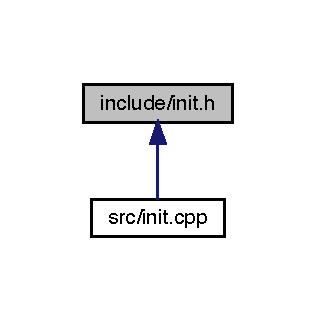
\includegraphics[width=152pt]{de/ddb/init_8h__dep__incl}
\end{center}
\end{figure}


\doxysubsection{Detailed Description}
Declares all the pre-\/autonomous functions for the robot

\begin{DoxyAuthor}{Author}
Michael Baraty 
\end{DoxyAuthor}
\begin{DoxyDate}{Date}
11/9/2019 
\end{DoxyDate}


Definition in file \mbox{\hyperlink{init_8h_source}{init.\+h}}.


\hypertarget{init_8h_source}{}\doxysection{init.\+h}
\label{init_8h_source}\index{include/init.h@{include/init.h}}

\begin{DoxyCode}{0}
\DoxyCodeLine{00001 }
\DoxyCodeLine{00007 \textcolor{preprocessor}{\#ifndef INIT\_H}}
\DoxyCodeLine{00008 \textcolor{preprocessor}{\#define INIT\_H}}
\DoxyCodeLine{00009 }
\DoxyCodeLine{00010 }
\DoxyCodeLine{00011 \textcolor{preprocessor}{\#endif}}

\end{DoxyCode}

\hypertarget{vex_8h}{}\doxysection{include/vex.h File Reference}
\label{vex_8h}\index{include/vex.h@{include/vex.h}}
{\ttfamily \#include $<$stdio.\+h$>$}\newline
{\ttfamily \#include $<$stdlib.\+h$>$}\newline
{\ttfamily \#include $<$string.\+h$>$}\newline
{\ttfamily \#include $<$math.\+h$>$}\newline
{\ttfamily \#include \char`\"{}v5.\+h\char`\"{}}\newline
{\ttfamily \#include \char`\"{}v5\+\_\+vcs.\+h\char`\"{}}\newline
Include dependency graph for vex.\+h\+:\nopagebreak
\begin{figure}[H]
\begin{center}
\leavevmode
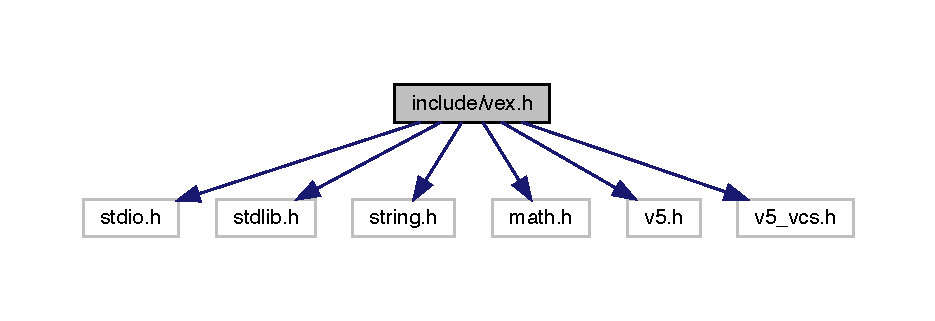
\includegraphics[width=350pt]{db/d70/vex_8h__incl}
\end{center}
\end{figure}
This graph shows which files directly or indirectly include this file\+:\nopagebreak
\begin{figure}[H]
\begin{center}
\leavevmode
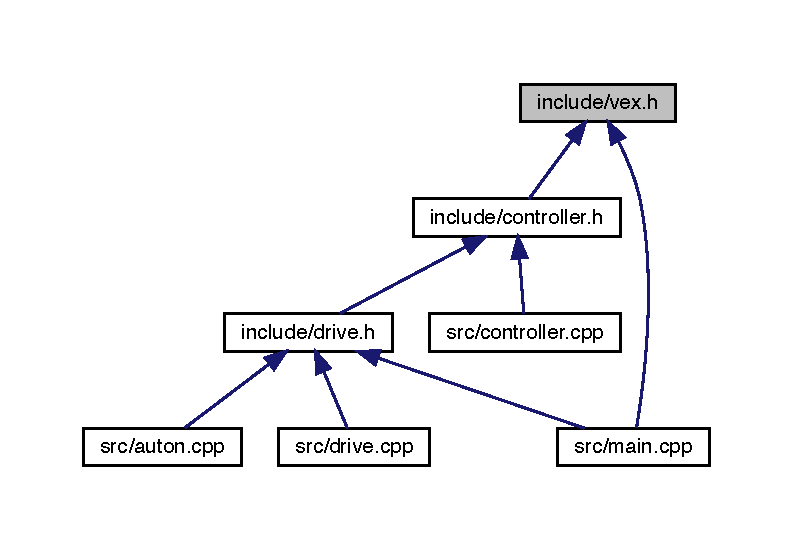
\includegraphics[width=350pt]{d8/d90/vex_8h__dep__incl}
\end{center}
\end{figure}

\hypertarget{vex_8h_source}{}\subsection{vex.\+h}
\label{vex_8h_source}\index{include/vex.\+h@{include/vex.\+h}}

\begin{DoxyCode}
00001 \textcolor{comment}{/*----------------------------------------------------------------------------*/}
00002 \textcolor{comment}{/*                                                                            */}
00003 \textcolor{comment}{/*    Module:       vex.h                                                     */}
00004 \textcolor{comment}{/*    Author:       Vex Robotics                                              */}
00005 \textcolor{comment}{/*    Created:      1 Feb 2019                                                */}
00006 \textcolor{comment}{/*    Description:  Default header for V5 projects                            */}
00007 \textcolor{comment}{/*                                                                            */}
00008 \textcolor{comment}{/*----------------------------------------------------------------------------*/}
00009 \textcolor{comment}{//}
00010 \textcolor{preprocessor}{#ifndef VEX\_H}
00011 \textcolor{preprocessor}{#define VEX\_H}
00012 
00013 
00014 \textcolor{preprocessor}{#include <stdio.h>}
00015 \textcolor{preprocessor}{#include <stdlib.h>}
00016 \textcolor{preprocessor}{#include <string.h>}
00017 \textcolor{preprocessor}{#include <math.h>}
00018 
00019 \textcolor{preprocessor}{#include "v5.h"}
00020 \textcolor{preprocessor}{#include "v5\_vcs.h"}
00021 
00022 \textcolor{preprocessor}{#endif}
\end{DoxyCode}

\hypertarget{auton_8cpp}{}\subsection{src/auton.cpp File Reference}
\label{auton_8cpp}\index{src/auton.\+cpp@{src/auton.\+cpp}}
{\ttfamily \#include \char`\"{}auton.\+h\char`\"{}}\newline
{\ttfamily \#include \char`\"{}drive.\+h\char`\"{}}\newline
{\ttfamily \#include \char`\"{}declarations.\+h\char`\"{}}\newline
\subsubsection*{Functions}
\begin{DoxyCompactItemize}
\item 
void \mbox{\hyperlink{auton_8cpp_ac132ca53625938c26d9d9104ca5c9e82}{move\+Forward}} (double inches)
\item 
void \mbox{\hyperlink{auton_8cpp_a7c81bf7b683346af95d1ff72eb60619f}{pivot\+Clockwise}} (float degrees)
\item 
void \mbox{\hyperlink{auton_8cpp_a962e4ac8747da1eb2aba6615d62e953b}{pivot\+Counter\+Clockwise}} (float degrees)
\item 
void \mbox{\hyperlink{auton_8cpp_a9c7e58a3b4bb5cdd30a6b3ed32e8f962}{auton}} (\mbox{\hyperlink{auton_8h_a702107095bd059695d57318e7338a4a7}{Side}} side, \mbox{\hyperlink{auton_8h_a78abb31bad0fd1834c54a3ca6f8daab5}{Color}} color)
\begin{DoxyCompactList}\small\item\em the autonomous switcher \end{DoxyCompactList}\item 
void \mbox{\hyperlink{auton_8cpp_a5bb01d00c76862cb15431efd4090bee9}{auton\+Blue\+Left}} ()
\item 
void \mbox{\hyperlink{auton_8cpp_ab9984e9a12048995fb71a06a1c94fd31}{auton\+Blue\+Right}} ()
\item 
void \mbox{\hyperlink{auton_8cpp_aae46c4423bc7ed2947e82c4c5dd7f469}{auton\+Red\+Left}} ()
\item 
void \mbox{\hyperlink{auton_8cpp_aaf3b274e9144b7072829ca58203492a6}{auton\+Red\+Right}} ()
\item 
void \mbox{\hyperlink{auton_8cpp_a1a25993901b668e4c162eb31fa463b52}{auton\+Start}} ()
\end{DoxyCompactItemize}


\subsubsection{Function Documentation}
\mbox{\Hypertarget{auton_8cpp_a9c7e58a3b4bb5cdd30a6b3ed32e8f962}\label{auton_8cpp_a9c7e58a3b4bb5cdd30a6b3ed32e8f962}} 
\index{auton.\+cpp@{auton.\+cpp}!auton@{auton}}
\index{auton@{auton}!auton.\+cpp@{auton.\+cpp}}
\paragraph{\texorpdfstring{auton()}{auton()}}
{\footnotesize\ttfamily void auton (\begin{DoxyParamCaption}\item[{\mbox{\hyperlink{auton_8h_a702107095bd059695d57318e7338a4a7}{Side}}}]{side,  }\item[{\mbox{\hyperlink{auton_8h_a78abb31bad0fd1834c54a3ca6f8daab5}{Color}}}]{color }\end{DoxyParamCaption})}



the autonomous switcher 

\begin{DoxyAuthor}{Author}
Michael Baraty 
\end{DoxyAuthor}


Definition at line 38 of file auton.\+cpp.

\mbox{\Hypertarget{auton_8cpp_a5bb01d00c76862cb15431efd4090bee9}\label{auton_8cpp_a5bb01d00c76862cb15431efd4090bee9}} 
\index{auton.\+cpp@{auton.\+cpp}!auton\+Blue\+Left@{auton\+Blue\+Left}}
\index{auton\+Blue\+Left@{auton\+Blue\+Left}!auton.\+cpp@{auton.\+cpp}}
\paragraph{\texorpdfstring{auton\+Blue\+Left()}{autonBlueLeft()}}
{\footnotesize\ttfamily void auton\+Blue\+Left (\begin{DoxyParamCaption}{ }\end{DoxyParamCaption})}

Initiates blue left autonomous routine \begin{DoxyAuthor}{Author}
Michael Baraty 
\end{DoxyAuthor}
\begin{DoxyDate}{Date}
11/9/2019 
\end{DoxyDate}


Definition at line 52 of file auton.\+cpp.

\mbox{\Hypertarget{auton_8cpp_ab9984e9a12048995fb71a06a1c94fd31}\label{auton_8cpp_ab9984e9a12048995fb71a06a1c94fd31}} 
\index{auton.\+cpp@{auton.\+cpp}!auton\+Blue\+Right@{auton\+Blue\+Right}}
\index{auton\+Blue\+Right@{auton\+Blue\+Right}!auton.\+cpp@{auton.\+cpp}}
\paragraph{\texorpdfstring{auton\+Blue\+Right()}{autonBlueRight()}}
{\footnotesize\ttfamily void auton\+Blue\+Right (\begin{DoxyParamCaption}{ }\end{DoxyParamCaption})}

Initiates blue right autonomous routine \begin{DoxyAuthor}{Author}
Michael Baraty 
\end{DoxyAuthor}
\begin{DoxyDate}{Date}
11/9/2019 
\end{DoxyDate}


Definition at line 56 of file auton.\+cpp.

\mbox{\Hypertarget{auton_8cpp_aae46c4423bc7ed2947e82c4c5dd7f469}\label{auton_8cpp_aae46c4423bc7ed2947e82c4c5dd7f469}} 
\index{auton.\+cpp@{auton.\+cpp}!auton\+Red\+Left@{auton\+Red\+Left}}
\index{auton\+Red\+Left@{auton\+Red\+Left}!auton.\+cpp@{auton.\+cpp}}
\paragraph{\texorpdfstring{auton\+Red\+Left()}{autonRedLeft()}}
{\footnotesize\ttfamily void auton\+Red\+Left (\begin{DoxyParamCaption}{ }\end{DoxyParamCaption})}

Initiates red left autonomous routine \begin{DoxyAuthor}{Author}
Michael Baraty 
\end{DoxyAuthor}
\begin{DoxyDate}{Date}
11/9/2019 
\end{DoxyDate}


Definition at line 60 of file auton.\+cpp.

\mbox{\Hypertarget{auton_8cpp_aaf3b274e9144b7072829ca58203492a6}\label{auton_8cpp_aaf3b274e9144b7072829ca58203492a6}} 
\index{auton.\+cpp@{auton.\+cpp}!auton\+Red\+Right@{auton\+Red\+Right}}
\index{auton\+Red\+Right@{auton\+Red\+Right}!auton.\+cpp@{auton.\+cpp}}
\paragraph{\texorpdfstring{auton\+Red\+Right()}{autonRedRight()}}
{\footnotesize\ttfamily void auton\+Red\+Right (\begin{DoxyParamCaption}{ }\end{DoxyParamCaption})}

Initiates red right autonomous routine \begin{DoxyAuthor}{Author}
Michael Baraty 
\end{DoxyAuthor}
\begin{DoxyDate}{Date}
11/9/2019 
\end{DoxyDate}


Definition at line 64 of file auton.\+cpp.

\mbox{\Hypertarget{auton_8cpp_a1a25993901b668e4c162eb31fa463b52}\label{auton_8cpp_a1a25993901b668e4c162eb31fa463b52}} 
\index{auton.\+cpp@{auton.\+cpp}!auton\+Start@{auton\+Start}}
\index{auton\+Start@{auton\+Start}!auton.\+cpp@{auton.\+cpp}}
\paragraph{\texorpdfstring{auton\+Start()}{autonStart()}}
{\footnotesize\ttfamily void auton\+Start (\begin{DoxyParamCaption}{ }\end{DoxyParamCaption})}


\begin{DoxyEnumerate}
\item Move intake up so mechanisms deploy
\item Move intake back down
\item Run intake and drive forward to pick up preload
\item Score cubes 
\end{DoxyEnumerate}

Definition at line 95 of file auton.\+cpp.

\mbox{\Hypertarget{auton_8cpp_ac132ca53625938c26d9d9104ca5c9e82}\label{auton_8cpp_ac132ca53625938c26d9d9104ca5c9e82}} 
\index{auton.\+cpp@{auton.\+cpp}!move\+Forward@{move\+Forward}}
\index{move\+Forward@{move\+Forward}!auton.\+cpp@{auton.\+cpp}}
\paragraph{\texorpdfstring{move\+Forward()}{moveForward()}}
{\footnotesize\ttfamily void move\+Forward (\begin{DoxyParamCaption}\item[{double}]{inches }\end{DoxyParamCaption})}

Declares the autonomous functions for the robot \begin{DoxyAuthor}{Author}
Michael Baraty 
\end{DoxyAuthor}
\begin{DoxyDate}{Date}
11/9/2019 Moves the robot forward for a certain distance 
\end{DoxyDate}

\begin{DoxyParams}{Parameters}
{\em inches} & The distance to move in inches (negative for reverse) \\
\hline
\end{DoxyParams}
\begin{DoxyAuthor}{Author}
Michael Baraty 
\end{DoxyAuthor}
\begin{DoxyDate}{Date}
11/9/2019 
\end{DoxyDate}


Definition at line 5 of file auton.\+cpp.

\mbox{\Hypertarget{auton_8cpp_a7c81bf7b683346af95d1ff72eb60619f}\label{auton_8cpp_a7c81bf7b683346af95d1ff72eb60619f}} 
\index{auton.\+cpp@{auton.\+cpp}!pivot\+Clockwise@{pivot\+Clockwise}}
\index{pivot\+Clockwise@{pivot\+Clockwise}!auton.\+cpp@{auton.\+cpp}}
\paragraph{\texorpdfstring{pivot\+Clockwise()}{pivotClockwise()}}
{\footnotesize\ttfamily void pivot\+Clockwise (\begin{DoxyParamCaption}\item[{float}]{degrees }\end{DoxyParamCaption})}

Pivots the robot clockwise to a certain angle 
\begin{DoxyParams}{Parameters}
{\em degrees} & The number of degrees to pivot the robot \\
\hline
\end{DoxyParams}
\begin{DoxyAuthor}{Author}
Michael Baraty 
\end{DoxyAuthor}
\begin{DoxyDate}{Date}
11/9/2019 
\end{DoxyDate}


Definition at line 14 of file auton.\+cpp.

\mbox{\Hypertarget{auton_8cpp_a962e4ac8747da1eb2aba6615d62e953b}\label{auton_8cpp_a962e4ac8747da1eb2aba6615d62e953b}} 
\index{auton.\+cpp@{auton.\+cpp}!pivot\+Counter\+Clockwise@{pivot\+Counter\+Clockwise}}
\index{pivot\+Counter\+Clockwise@{pivot\+Counter\+Clockwise}!auton.\+cpp@{auton.\+cpp}}
\paragraph{\texorpdfstring{pivot\+Counter\+Clockwise()}{pivotCounterClockwise()}}
{\footnotesize\ttfamily void pivot\+Counter\+Clockwise (\begin{DoxyParamCaption}\item[{float}]{degrees }\end{DoxyParamCaption})}

Pivots the robot counter-\/clockwise to a certain angle 
\begin{DoxyParams}{Parameters}
{\em degrees} & The number of degrees to pivot the robot \\
\hline
\end{DoxyParams}
\begin{DoxyAuthor}{Author}
Michael Baraty 
\end{DoxyAuthor}
\begin{DoxyDate}{Date}
11/9/2019 
\end{DoxyDate}


Definition at line 24 of file auton.\+cpp.


\hypertarget{auton_8cpp_source}{}\doxysection{auton.\+cpp}
\label{auton_8cpp_source}\index{src/auton.cpp@{src/auton.cpp}}

\begin{DoxyCode}{0}
\DoxyCodeLine{00001 \textcolor{preprocessor}{\#include "\mbox{\hyperlink{auton_8h}{auton.h}}"}}
\DoxyCodeLine{00002 \textcolor{preprocessor}{\#include "\mbox{\hyperlink{drive_8h}{drive.h}}"}}
\DoxyCodeLine{00003 \textcolor{preprocessor}{\#include "\mbox{\hyperlink{declarations_8h}{declarations.h}}"}}
\DoxyCodeLine{00004 }
\DoxyCodeLine{\Hypertarget{auton_8cpp_source_l00005}\mbox{\hyperlink{auton_8cpp_af5833bec4b862d3da7fc3700ca7d2a6b_af5833bec4b862d3da7fc3700ca7d2a6b}{00005}} \textcolor{keywordtype}{bool} \mbox{\hyperlink{auton_8cpp_af5833bec4b862d3da7fc3700ca7d2a6b_af5833bec4b862d3da7fc3700ca7d2a6b}{moveForward}}(\textcolor{keywordtype}{double} inches, \textcolor{keywordtype}{double} speed = 50, \textcolor{keywordtype}{bool} blocking = \textcolor{keyword}{true}) \{}
\DoxyCodeLine{00006 }
\DoxyCodeLine{00007 }
\DoxyCodeLine{00008   \textcolor{keywordtype}{double} rotations = inches * \mbox{\hyperlink{declarations_8h_acfdb8ffd7cd602577173adb1c9c0f330_acfdb8ffd7cd602577173adb1c9c0f330}{ROTATIONS\_PER\_INCH}};}
\DoxyCodeLine{00009   \textcolor{keywordflow}{if}(blocking) \{}
\DoxyCodeLine{00010     \mbox{\hyperlink{declarations_8h_ab24214b642128d0f3cb67e9b12e7d4fb_ab24214b642128d0f3cb67e9b12e7d4fb}{MOTOR\_BACK\_LEFT}}.startRotateFor(directionType::fwd, rotations, rotationUnits::rev, speed, velocityUnits::pct);}
\DoxyCodeLine{00011     \mbox{\hyperlink{declarations_8h_adece81dedf91c2893ba42dc05135a575_adece81dedf91c2893ba42dc05135a575}{MOTOR\_BACK\_RIGHT}}.startRotateFor(directionType::fwd, rotations, rotationUnits::rev, speed, velocityUnits::pct);}
\DoxyCodeLine{00012     \mbox{\hyperlink{declarations_8h_a8c6f6315caf1d81bf4d4d113d0f7bffc_a8c6f6315caf1d81bf4d4d113d0f7bffc}{MOTOR\_FRONT\_LEFT}}.startRotateFor(directionType::fwd, rotations, rotationUnits::rev, speed, velocityUnits::pct);}
\DoxyCodeLine{00013     \mbox{\hyperlink{declarations_8h_ad6a9ea3d338421c5d709c32ae1aa42d8_ad6a9ea3d338421c5d709c32ae1aa42d8}{MOTOR\_FRONT\_RIGHT}}.rotateFor(directionType::fwd, rotations, rotationUnits::rev, speed, velocityUnits::pct);}
\DoxyCodeLine{00014   \} \textcolor{keywordflow}{else} \{}
\DoxyCodeLine{00015     \mbox{\hyperlink{declarations_8h_ab24214b642128d0f3cb67e9b12e7d4fb_ab24214b642128d0f3cb67e9b12e7d4fb}{MOTOR\_BACK\_LEFT}}.startRotateFor(directionType::fwd, rotations, rotationUnits::rev, speed, velocityUnits::pct);}
\DoxyCodeLine{00016     \mbox{\hyperlink{declarations_8h_adece81dedf91c2893ba42dc05135a575_adece81dedf91c2893ba42dc05135a575}{MOTOR\_BACK\_RIGHT}}.startRotateFor(directionType::fwd, rotations, rotationUnits::rev, speed, velocityUnits::pct);}
\DoxyCodeLine{00017     \mbox{\hyperlink{declarations_8h_a8c6f6315caf1d81bf4d4d113d0f7bffc_a8c6f6315caf1d81bf4d4d113d0f7bffc}{MOTOR\_FRONT\_LEFT}}.startRotateFor(directionType::fwd, rotations, rotationUnits::rev, speed, velocityUnits::pct);}
\DoxyCodeLine{00018     \mbox{\hyperlink{declarations_8h_ad6a9ea3d338421c5d709c32ae1aa42d8_ad6a9ea3d338421c5d709c32ae1aa42d8}{MOTOR\_FRONT\_RIGHT}}.startRotateFor(directionType::fwd, rotations, rotationUnits::rev, speed, velocityUnits::pct);}
\DoxyCodeLine{00019   \}}
\DoxyCodeLine{00020   \textcolor{keywordflow}{return} \textcolor{keyword}{true};}
\DoxyCodeLine{00021 \}}
\DoxyCodeLine{00022 }
\DoxyCodeLine{\Hypertarget{auton_8cpp_source_l00023}\mbox{\hyperlink{auton_8cpp_a362446334157b1edf93062607b0f5e4c_a362446334157b1edf93062607b0f5e4c}{00023}} \textcolor{keywordtype}{bool} \mbox{\hyperlink{auton_8cpp_a362446334157b1edf93062607b0f5e4c_a362446334157b1edf93062607b0f5e4c}{pivotClockwise}}(\textcolor{keywordtype}{float} degrees, \textcolor{keywordtype}{bool} blocking = \textcolor{keyword}{true}) \{}
\DoxyCodeLine{00024   \textcolor{keywordtype}{double} rotations\_per\_360 = 6.4;}
\DoxyCodeLine{00025   \textcolor{keywordtype}{double} rotations = rotations\_per\_360 * (degrees / 360);}
\DoxyCodeLine{00026 }
\DoxyCodeLine{00027   \textcolor{keywordflow}{if}(blocking)\{}
\DoxyCodeLine{00028   \mbox{\hyperlink{declarations_8h_ab24214b642128d0f3cb67e9b12e7d4fb_ab24214b642128d0f3cb67e9b12e7d4fb}{MOTOR\_BACK\_LEFT}}.startRotateFor(rotations, rotationUnits::rev, 80, velocityUnits::pct);}
\DoxyCodeLine{00029   \mbox{\hyperlink{declarations_8h_adece81dedf91c2893ba42dc05135a575_adece81dedf91c2893ba42dc05135a575}{MOTOR\_BACK\_RIGHT}}.startRotateFor(-\/rotations, rotationUnits::rev, 80, velocityUnits::pct);}
\DoxyCodeLine{00030   \mbox{\hyperlink{declarations_8h_a8c6f6315caf1d81bf4d4d113d0f7bffc_a8c6f6315caf1d81bf4d4d113d0f7bffc}{MOTOR\_FRONT\_LEFT}}.startRotateFor(rotations, rotationUnits::rev, 80, velocityUnits::pct);}
\DoxyCodeLine{00031   \mbox{\hyperlink{declarations_8h_ad6a9ea3d338421c5d709c32ae1aa42d8_ad6a9ea3d338421c5d709c32ae1aa42d8}{MOTOR\_FRONT\_RIGHT}}.rotateFor(-\/rotations, rotationUnits::rev, 80, velocityUnits::pct);}
\DoxyCodeLine{00032   \} \textcolor{keywordflow}{else} \{}
\DoxyCodeLine{00033     \mbox{\hyperlink{declarations_8h_ab24214b642128d0f3cb67e9b12e7d4fb_ab24214b642128d0f3cb67e9b12e7d4fb}{MOTOR\_BACK\_LEFT}}.startRotateFor(rotations, rotationUnits::rev, 80, velocityUnits::pct);}
\DoxyCodeLine{00034     \mbox{\hyperlink{declarations_8h_adece81dedf91c2893ba42dc05135a575_adece81dedf91c2893ba42dc05135a575}{MOTOR\_BACK\_RIGHT}}.startRotateFor(-\/rotations, rotationUnits::rev, 80, velocityUnits::pct);}
\DoxyCodeLine{00035     \mbox{\hyperlink{declarations_8h_a8c6f6315caf1d81bf4d4d113d0f7bffc_a8c6f6315caf1d81bf4d4d113d0f7bffc}{MOTOR\_FRONT\_LEFT}}.startRotateFor(rotations, rotationUnits::rev, 80, velocityUnits::pct);}
\DoxyCodeLine{00036     \mbox{\hyperlink{declarations_8h_ad6a9ea3d338421c5d709c32ae1aa42d8_ad6a9ea3d338421c5d709c32ae1aa42d8}{MOTOR\_FRONT\_RIGHT}}.startRotateFor(-\/rotations, rotationUnits::rev, 80, velocityUnits::pct);}
\DoxyCodeLine{00037   \}}
\DoxyCodeLine{00038 }
\DoxyCodeLine{00039   \textcolor{keywordflow}{return} \textcolor{keyword}{true};}
\DoxyCodeLine{00040 \}}
\DoxyCodeLine{00041 }
\DoxyCodeLine{\Hypertarget{auton_8cpp_source_l00042}\mbox{\hyperlink{auton_8cpp_a241030fa952d5f1fdbe92a97a20e6a36_a241030fa952d5f1fdbe92a97a20e6a36}{00042}} \textcolor{keywordtype}{bool} \mbox{\hyperlink{auton_8cpp_a241030fa952d5f1fdbe92a97a20e6a36_a241030fa952d5f1fdbe92a97a20e6a36}{pivotCounterClockwise}}(\textcolor{keywordtype}{float} degrees, \textcolor{keywordtype}{bool} blocking = \textcolor{keyword}{true}) \{}
\DoxyCodeLine{00043   \textcolor{keywordtype}{double} rotations\_per\_360 = 6.4;}
\DoxyCodeLine{00044   \textcolor{keywordtype}{double} rotations = rotations\_per\_360 * (degrees / 360);}
\DoxyCodeLine{00045 }
\DoxyCodeLine{00046   \textcolor{keywordflow}{if}(blocking) \{}
\DoxyCodeLine{00047   \mbox{\hyperlink{declarations_8h_ab24214b642128d0f3cb67e9b12e7d4fb_ab24214b642128d0f3cb67e9b12e7d4fb}{MOTOR\_BACK\_LEFT}}.startRotateFor(-\/rotations, rotationUnits::rev, 80, velocityUnits::pct);}
\DoxyCodeLine{00048   \mbox{\hyperlink{declarations_8h_adece81dedf91c2893ba42dc05135a575_adece81dedf91c2893ba42dc05135a575}{MOTOR\_BACK\_RIGHT}}.startRotateFor(rotations, rotationUnits::rev, 80, velocityUnits::pct);}
\DoxyCodeLine{00049   \mbox{\hyperlink{declarations_8h_a8c6f6315caf1d81bf4d4d113d0f7bffc_a8c6f6315caf1d81bf4d4d113d0f7bffc}{MOTOR\_FRONT\_LEFT}}.startRotateFor(-\/rotations, rotationUnits::rev, 80, velocityUnits::pct);}
\DoxyCodeLine{00050   \mbox{\hyperlink{declarations_8h_ad6a9ea3d338421c5d709c32ae1aa42d8_ad6a9ea3d338421c5d709c32ae1aa42d8}{MOTOR\_FRONT\_RIGHT}}.rotateFor(rotations, rotationUnits::rev, 80, velocityUnits::pct);}
\DoxyCodeLine{00051   \} \textcolor{keywordflow}{else} \{}
\DoxyCodeLine{00052     \mbox{\hyperlink{declarations_8h_ab24214b642128d0f3cb67e9b12e7d4fb_ab24214b642128d0f3cb67e9b12e7d4fb}{MOTOR\_BACK\_LEFT}}.startRotateFor(-\/rotations, rotationUnits::rev, 80, velocityUnits::pct);}
\DoxyCodeLine{00053   \mbox{\hyperlink{declarations_8h_adece81dedf91c2893ba42dc05135a575_adece81dedf91c2893ba42dc05135a575}{MOTOR\_BACK\_RIGHT}}.startRotateFor(rotations, rotationUnits::rev, 80, velocityUnits::pct);}
\DoxyCodeLine{00054   \mbox{\hyperlink{declarations_8h_a8c6f6315caf1d81bf4d4d113d0f7bffc_a8c6f6315caf1d81bf4d4d113d0f7bffc}{MOTOR\_FRONT\_LEFT}}.startRotateFor(-\/rotations, rotationUnits::rev, 80, velocityUnits::pct);}
\DoxyCodeLine{00055   \mbox{\hyperlink{declarations_8h_ad6a9ea3d338421c5d709c32ae1aa42d8_ad6a9ea3d338421c5d709c32ae1aa42d8}{MOTOR\_FRONT\_RIGHT}}.startRotateFor(rotations, rotationUnits::rev, 80, velocityUnits::pct);}
\DoxyCodeLine{00056   \}}
\DoxyCodeLine{00057   \textcolor{keywordflow}{return} \textcolor{keyword}{true};}
\DoxyCodeLine{00058 \}}
\DoxyCodeLine{00059 }
\DoxyCodeLine{\Hypertarget{auton_8cpp_source_l00064}\mbox{\hyperlink{auton_8cpp_a9c7e58a3b4bb5cdd30a6b3ed32e8f962_a9c7e58a3b4bb5cdd30a6b3ed32e8f962}{00064}} \textcolor{keywordtype}{void} \mbox{\hyperlink{auton_8cpp_a9c7e58a3b4bb5cdd30a6b3ed32e8f962_a9c7e58a3b4bb5cdd30a6b3ed32e8f962}{auton}}(\mbox{\hyperlink{auton_8h_a702107095bd059695d57318e7338a4a7_a702107095bd059695d57318e7338a4a7}{Side}} side, \mbox{\hyperlink{auton_8h_a78abb31bad0fd1834c54a3ca6f8daab5_a78abb31bad0fd1834c54a3ca6f8daab5}{Color}} color) \{}
\DoxyCodeLine{00065   \mbox{\hyperlink{auton_8cpp_abba3fa3f69d7ee97541aa1169ee13cee_abba3fa3f69d7ee97541aa1169ee13cee}{autonStart}}();}
\DoxyCodeLine{00066 }
\DoxyCodeLine{00067   \textcolor{keywordflow}{if}(color == \mbox{\hyperlink{auton_8h_a78abb31bad0fd1834c54a3ca6f8daab5_a78abb31bad0fd1834c54a3ca6f8daab5a1b3e1ee9bff86431dea6b181365ba65f}{Color::BLUE}} \&\& side == \mbox{\hyperlink{auton_8h_a702107095bd059695d57318e7338a4a7_a702107095bd059695d57318e7338a4a7a684d325a7303f52e64011467ff5c5758}{Side::LEFT}})}
\DoxyCodeLine{00068     \mbox{\hyperlink{auton_8cpp_a5bb01d00c76862cb15431efd4090bee9_a5bb01d00c76862cb15431efd4090bee9}{autonBlueLeft}}();}
\DoxyCodeLine{00069   \textcolor{keywordflow}{else} \textcolor{keywordflow}{if} (color == \mbox{\hyperlink{auton_8h_a78abb31bad0fd1834c54a3ca6f8daab5_a78abb31bad0fd1834c54a3ca6f8daab5a1b3e1ee9bff86431dea6b181365ba65f}{Color::BLUE}} \&\& side == \mbox{\hyperlink{auton_8h_a702107095bd059695d57318e7338a4a7_a702107095bd059695d57318e7338a4a7a21507b40c80068eda19865706fdc2403}{Side::RIGHT}})}
\DoxyCodeLine{00070     \mbox{\hyperlink{auton_8cpp_ab9984e9a12048995fb71a06a1c94fd31_ab9984e9a12048995fb71a06a1c94fd31}{autonBlueRight}}();}
\DoxyCodeLine{00071   \textcolor{keywordflow}{else} \textcolor{keywordflow}{if} (color == \mbox{\hyperlink{auton_8h_a78abb31bad0fd1834c54a3ca6f8daab5_a78abb31bad0fd1834c54a3ca6f8daab5aa2d9547b5d3dd9f05984475f7c926da0}{Color::RED}} \&\& side == \mbox{\hyperlink{auton_8h_a702107095bd059695d57318e7338a4a7_a702107095bd059695d57318e7338a4a7a684d325a7303f52e64011467ff5c5758}{Side::LEFT}})}
\DoxyCodeLine{00072     \mbox{\hyperlink{auton_8cpp_aae46c4423bc7ed2947e82c4c5dd7f469_aae46c4423bc7ed2947e82c4c5dd7f469}{autonRedLeft}}();}
\DoxyCodeLine{00073   \textcolor{keywordflow}{else} \textcolor{keywordflow}{if} (color == \mbox{\hyperlink{auton_8h_a78abb31bad0fd1834c54a3ca6f8daab5_a78abb31bad0fd1834c54a3ca6f8daab5aa2d9547b5d3dd9f05984475f7c926da0}{Color::RED}} \&\& side == \mbox{\hyperlink{auton_8h_a702107095bd059695d57318e7338a4a7_a702107095bd059695d57318e7338a4a7a21507b40c80068eda19865706fdc2403}{Side::RIGHT}})}
\DoxyCodeLine{00074     \mbox{\hyperlink{auton_8cpp_aaf3b274e9144b7072829ca58203492a6_aaf3b274e9144b7072829ca58203492a6}{autonRedRight}}();}
\DoxyCodeLine{00075 \}}
\DoxyCodeLine{00076 }
\DoxyCodeLine{00077 }
\DoxyCodeLine{\Hypertarget{auton_8cpp_source_l00078}\mbox{\hyperlink{auton_8cpp_a5bb01d00c76862cb15431efd4090bee9_a5bb01d00c76862cb15431efd4090bee9}{00078}} \textcolor{keywordtype}{void} \mbox{\hyperlink{auton_8cpp_a5bb01d00c76862cb15431efd4090bee9_a5bb01d00c76862cb15431efd4090bee9}{autonBlueLeft}}()\{}
\DoxyCodeLine{00079   \mbox{\hyperlink{declarations_8h_a34de211d15bfb3c0ac450597fd96b4fc_a34de211d15bfb3c0ac450597fd96b4fc}{MOTOR\_INTAKE\_A}}.startRotateFor(7, rotationUnits::rev, 100, velocityUnits::pct);}
\DoxyCodeLine{00080   \mbox{\hyperlink{declarations_8h_a5ae79e7ed71b0b94b3983c22c60c2eaa_a5ae79e7ed71b0b94b3983c22c60c2eaa}{MOTOR\_INTAKE\_B}}.startRotateFor(7, rotationUnits::rev, 100, velocityUnits::pct);}
\DoxyCodeLine{00081   \mbox{\hyperlink{auton_8cpp_af5833bec4b862d3da7fc3700ca7d2a6b_af5833bec4b862d3da7fc3700ca7d2a6b}{moveForward}}(35, 33);}
\DoxyCodeLine{00082   \textcolor{comment}{/*pivotClockwise(190);}}
\DoxyCodeLine{00083 \textcolor{comment}{  moveForward(24);}}
\DoxyCodeLine{00084 \textcolor{comment}{  pivotCounterClockwise(45);*/}}
\DoxyCodeLine{00085   \mbox{\hyperlink{auton_8cpp_af5833bec4b862d3da7fc3700ca7d2a6b_af5833bec4b862d3da7fc3700ca7d2a6b}{moveForward}}(-\/24, 60);}
\DoxyCodeLine{00086   \mbox{\hyperlink{auton_8cpp_a241030fa952d5f1fdbe92a97a20e6a36_a241030fa952d5f1fdbe92a97a20e6a36}{pivotCounterClockwise}}(135);}
\DoxyCodeLine{00087   \mbox{\hyperlink{auton_8cpp_af5833bec4b862d3da7fc3700ca7d2a6b_af5833bec4b862d3da7fc3700ca7d2a6b}{moveForward}}(10);}
\DoxyCodeLine{00088   \mbox{\hyperlink{auton_8cpp_af5833bec4b862d3da7fc3700ca7d2a6b_af5833bec4b862d3da7fc3700ca7d2a6b}{moveForward}}(5, 30, \textcolor{keyword}{false});}
\DoxyCodeLine{00089   \mbox{\hyperlink{declarations_8h_a34de211d15bfb3c0ac450597fd96b4fc_a34de211d15bfb3c0ac450597fd96b4fc}{MOTOR\_INTAKE\_A}}.startRotateFor(-\/.5, rotationUnits::rev, 100, velocityUnits::pct);}
\DoxyCodeLine{00090   \mbox{\hyperlink{declarations_8h_a5ae79e7ed71b0b94b3983c22c60c2eaa_a5ae79e7ed71b0b94b3983c22c60c2eaa}{MOTOR\_INTAKE\_B}}.startRotateFor(-\/.5, rotationUnits::rev, 100, velocityUnits::pct);}
\DoxyCodeLine{00091   \mbox{\hyperlink{declarations_8h_a212c888d64ffcd7e7b44a548fa0408a9_a212c888d64ffcd7e7b44a548fa0408a9}{MOTOR\_STACK}}.rotateFor(2, rev);}
\DoxyCodeLine{00092   \mbox{\hyperlink{declarations_8h_a34de211d15bfb3c0ac450597fd96b4fc_a34de211d15bfb3c0ac450597fd96b4fc}{MOTOR\_INTAKE\_A}}.startRotateFor(-\/20, rotationUnits::rev, 100, velocityUnits::pct);}
\DoxyCodeLine{00093   \mbox{\hyperlink{declarations_8h_a5ae79e7ed71b0b94b3983c22c60c2eaa_a5ae79e7ed71b0b94b3983c22c60c2eaa}{MOTOR\_INTAKE\_B}}.startRotateFor(-\/20, rotationUnits::rev, 100, velocityUnits::pct);}
\DoxyCodeLine{00094   \mbox{\hyperlink{auton_8cpp_af5833bec4b862d3da7fc3700ca7d2a6b_af5833bec4b862d3da7fc3700ca7d2a6b}{moveForward}}(-\/20, 33);}
\DoxyCodeLine{00095   \mbox{\hyperlink{declarations_8h_a34de211d15bfb3c0ac450597fd96b4fc_a34de211d15bfb3c0ac450597fd96b4fc}{MOTOR\_INTAKE\_A}}.stop();}
\DoxyCodeLine{00096   \mbox{\hyperlink{declarations_8h_a5ae79e7ed71b0b94b3983c22c60c2eaa_a5ae79e7ed71b0b94b3983c22c60c2eaa}{MOTOR\_INTAKE\_B}}.stop();}
\DoxyCodeLine{00097 \}}
\DoxyCodeLine{00098 }
\DoxyCodeLine{\Hypertarget{auton_8cpp_source_l00099}\mbox{\hyperlink{auton_8cpp_ab9984e9a12048995fb71a06a1c94fd31_ab9984e9a12048995fb71a06a1c94fd31}{00099}} \textcolor{keywordtype}{void} \mbox{\hyperlink{auton_8cpp_ab9984e9a12048995fb71a06a1c94fd31_ab9984e9a12048995fb71a06a1c94fd31}{autonBlueRight}}()\{}
\DoxyCodeLine{00100   \mbox{\hyperlink{drive_8h_aa0846c73538fc48569a7c7c3689a59f0_aa0846c73538fc48569a7c7c3689a59f0}{intakeIn}}();}
\DoxyCodeLine{00101   \mbox{\hyperlink{auton_8cpp_af5833bec4b862d3da7fc3700ca7d2a6b_af5833bec4b862d3da7fc3700ca7d2a6b}{moveForward}}(25, 70);}
\DoxyCodeLine{00102   \mbox{\hyperlink{auton_8cpp_af5833bec4b862d3da7fc3700ca7d2a6b_af5833bec4b862d3da7fc3700ca7d2a6b}{moveForward}}(12, 40);}
\DoxyCodeLine{00103   vexDelay(1000);}
\DoxyCodeLine{00104   \mbox{\hyperlink{declarations_8h_a34de211d15bfb3c0ac450597fd96b4fc_a34de211d15bfb3c0ac450597fd96b4fc}{MOTOR\_INTAKE\_A}}.stop(hold);}
\DoxyCodeLine{00105   \mbox{\hyperlink{declarations_8h_a5ae79e7ed71b0b94b3983c22c60c2eaa_a5ae79e7ed71b0b94b3983c22c60c2eaa}{MOTOR\_INTAKE\_B}}.stop(hold);}
\DoxyCodeLine{00106   \mbox{\hyperlink{auton_8cpp_af5833bec4b862d3da7fc3700ca7d2a6b_af5833bec4b862d3da7fc3700ca7d2a6b}{moveForward}}(-\/28, 80);}
\DoxyCodeLine{00107   \mbox{\hyperlink{auton_8cpp_a362446334157b1edf93062607b0f5e4c_a362446334157b1edf93062607b0f5e4c}{pivotClockwise}}(130);}
\DoxyCodeLine{00108   \mbox{\hyperlink{auton_8cpp_af5833bec4b862d3da7fc3700ca7d2a6b_af5833bec4b862d3da7fc3700ca7d2a6b}{moveForward}}(29, 50);}
\DoxyCodeLine{00109   \textcolor{comment}{//MOTOR\_INTAKE\_A.rotateFor(-\/.25, rotationUnits::rev, 100, velocityUnits::pct);}}
\DoxyCodeLine{00110   \textcolor{comment}{//MOTOR\_INTAKE\_B.rotateFor(-\/.25, rotationUnits::rev, 100, velocityUnits::pct);}}
\DoxyCodeLine{00111   \textcolor{comment}{//MOTOR\_STACK.startRotateTo(2.9, rotationUnits::rev);}}
\DoxyCodeLine{00112   \textcolor{comment}{//vexDelay(1500);}}
\DoxyCodeLine{00113   }
\DoxyCodeLine{00114   \mbox{\hyperlink{declarations_8h_a34de211d15bfb3c0ac450597fd96b4fc_a34de211d15bfb3c0ac450597fd96b4fc}{MOTOR\_INTAKE\_A}}.startRotateFor(-\/10, rotationUnits::rev, 100, velocityUnits::pct);}
\DoxyCodeLine{00115   \mbox{\hyperlink{declarations_8h_a5ae79e7ed71b0b94b3983c22c60c2eaa_a5ae79e7ed71b0b94b3983c22c60c2eaa}{MOTOR\_INTAKE\_B}}.startRotateFor(-\/10, rotationUnits::rev, 100, velocityUnits::pct);}
\DoxyCodeLine{00116   \mbox{\hyperlink{auton_8cpp_a362446334157b1edf93062607b0f5e4c_a362446334157b1edf93062607b0f5e4c}{pivotClockwise}}(60, \textcolor{keyword}{true});}
\DoxyCodeLine{00117 }
\DoxyCodeLine{00118   \mbox{\hyperlink{auton_8cpp_af5833bec4b862d3da7fc3700ca7d2a6b_af5833bec4b862d3da7fc3700ca7d2a6b}{moveForward}}(-\/13, 33, \textcolor{keyword}{true});}
\DoxyCodeLine{00119   }
\DoxyCodeLine{00120   \mbox{\hyperlink{declarations_8h_a212c888d64ffcd7e7b44a548fa0408a9_a212c888d64ffcd7e7b44a548fa0408a9}{MOTOR\_STACK}}.rotateTo(0, rotationUnits::rev, 80, velocityUnits::pct);}
\DoxyCodeLine{00121 \}}
\DoxyCodeLine{00122 }
\DoxyCodeLine{\Hypertarget{auton_8cpp_source_l00123}\mbox{\hyperlink{auton_8cpp_aae46c4423bc7ed2947e82c4c5dd7f469_aae46c4423bc7ed2947e82c4c5dd7f469}{00123}} \textcolor{keywordtype}{void} \mbox{\hyperlink{auton_8cpp_aae46c4423bc7ed2947e82c4c5dd7f469_aae46c4423bc7ed2947e82c4c5dd7f469}{autonRedLeft}}()\{}
\DoxyCodeLine{00124   \mbox{\hyperlink{drive_8h_aa0846c73538fc48569a7c7c3689a59f0_aa0846c73538fc48569a7c7c3689a59f0}{intakeIn}}();}
\DoxyCodeLine{00125   \mbox{\hyperlink{auton_8cpp_af5833bec4b862d3da7fc3700ca7d2a6b_af5833bec4b862d3da7fc3700ca7d2a6b}{moveForward}}(25, 70);}
\DoxyCodeLine{00126   \mbox{\hyperlink{auton_8cpp_af5833bec4b862d3da7fc3700ca7d2a6b_af5833bec4b862d3da7fc3700ca7d2a6b}{moveForward}}(12, 40);}
\DoxyCodeLine{00127   vexDelay(1000);}
\DoxyCodeLine{00128   \mbox{\hyperlink{declarations_8h_a34de211d15bfb3c0ac450597fd96b4fc_a34de211d15bfb3c0ac450597fd96b4fc}{MOTOR\_INTAKE\_A}}.stop(hold);}
\DoxyCodeLine{00129   \mbox{\hyperlink{declarations_8h_a5ae79e7ed71b0b94b3983c22c60c2eaa_a5ae79e7ed71b0b94b3983c22c60c2eaa}{MOTOR\_INTAKE\_B}}.stop(hold);}
\DoxyCodeLine{00130   \mbox{\hyperlink{auton_8cpp_af5833bec4b862d3da7fc3700ca7d2a6b_af5833bec4b862d3da7fc3700ca7d2a6b}{moveForward}}(-\/28, 80);}
\DoxyCodeLine{00131   \mbox{\hyperlink{auton_8cpp_a241030fa952d5f1fdbe92a97a20e6a36_a241030fa952d5f1fdbe92a97a20e6a36}{pivotCounterClockwise}}(130);}
\DoxyCodeLine{00132   \mbox{\hyperlink{auton_8cpp_af5833bec4b862d3da7fc3700ca7d2a6b_af5833bec4b862d3da7fc3700ca7d2a6b}{moveForward}}(29, 50);}
\DoxyCodeLine{00133   \textcolor{comment}{//MOTOR\_INTAKE\_A.rotateFor(-\/.25, rotationUnits::rev, 100, velocityUnits::pct);}}
\DoxyCodeLine{00134   \textcolor{comment}{//MOTOR\_INTAKE\_B.rotateFor(-\/.25, rotationUnits::rev, 100, velocityUnits::pct);}}
\DoxyCodeLine{00135   \textcolor{comment}{//MOTOR\_STACK.startRotateTo(2.9, rotationUnits::rev);}}
\DoxyCodeLine{00136   \textcolor{comment}{//vexDelay(1500);}}
\DoxyCodeLine{00137   }
\DoxyCodeLine{00138   \mbox{\hyperlink{declarations_8h_a34de211d15bfb3c0ac450597fd96b4fc_a34de211d15bfb3c0ac450597fd96b4fc}{MOTOR\_INTAKE\_A}}.startRotateFor(-\/10, rotationUnits::rev, 100, velocityUnits::pct);}
\DoxyCodeLine{00139   \mbox{\hyperlink{declarations_8h_a5ae79e7ed71b0b94b3983c22c60c2eaa_a5ae79e7ed71b0b94b3983c22c60c2eaa}{MOTOR\_INTAKE\_B}}.startRotateFor(-\/10, rotationUnits::rev, 100, velocityUnits::pct);}
\DoxyCodeLine{00140   \mbox{\hyperlink{auton_8cpp_a241030fa952d5f1fdbe92a97a20e6a36_a241030fa952d5f1fdbe92a97a20e6a36}{pivotCounterClockwise}}(60, \textcolor{keyword}{true});}
\DoxyCodeLine{00141   }
\DoxyCodeLine{00142   \mbox{\hyperlink{auton_8cpp_af5833bec4b862d3da7fc3700ca7d2a6b_af5833bec4b862d3da7fc3700ca7d2a6b}{moveForward}}(-\/13, 33, \textcolor{keyword}{true});}
\DoxyCodeLine{00143   }
\DoxyCodeLine{00144   \mbox{\hyperlink{declarations_8h_a212c888d64ffcd7e7b44a548fa0408a9_a212c888d64ffcd7e7b44a548fa0408a9}{MOTOR\_STACK}}.rotateTo(0, rotationUnits::rev, 80, velocityUnits::pct);}
\DoxyCodeLine{00145 \}}
\DoxyCodeLine{00146 }
\DoxyCodeLine{\Hypertarget{auton_8cpp_source_l00147}\mbox{\hyperlink{auton_8cpp_aaf3b274e9144b7072829ca58203492a6_aaf3b274e9144b7072829ca58203492a6}{00147}} \textcolor{keywordtype}{void} \mbox{\hyperlink{auton_8cpp_aaf3b274e9144b7072829ca58203492a6_aaf3b274e9144b7072829ca58203492a6}{autonRedRight}}()\{}
\DoxyCodeLine{00148   \mbox{\hyperlink{declarations_8h_a34de211d15bfb3c0ac450597fd96b4fc_a34de211d15bfb3c0ac450597fd96b4fc}{MOTOR\_INTAKE\_A}}.startRotateFor(7, rotationUnits::rev, 100, velocityUnits::pct);}
\DoxyCodeLine{00149   \mbox{\hyperlink{declarations_8h_a5ae79e7ed71b0b94b3983c22c60c2eaa_a5ae79e7ed71b0b94b3983c22c60c2eaa}{MOTOR\_INTAKE\_B}}.startRotateFor(7, rotationUnits::rev, 100, velocityUnits::pct);}
\DoxyCodeLine{00150   \mbox{\hyperlink{auton_8cpp_af5833bec4b862d3da7fc3700ca7d2a6b_af5833bec4b862d3da7fc3700ca7d2a6b}{moveForward}}(35, 33);}
\DoxyCodeLine{00151   \textcolor{comment}{/*pivotClockwise(190);}}
\DoxyCodeLine{00152 \textcolor{comment}{  moveForward(24);}}
\DoxyCodeLine{00153 \textcolor{comment}{  pivotCounterClockwise(45);*/}}
\DoxyCodeLine{00154   \mbox{\hyperlink{auton_8cpp_af5833bec4b862d3da7fc3700ca7d2a6b_af5833bec4b862d3da7fc3700ca7d2a6b}{moveForward}}(-\/24, 60);}
\DoxyCodeLine{00155   \mbox{\hyperlink{auton_8cpp_a362446334157b1edf93062607b0f5e4c_a362446334157b1edf93062607b0f5e4c}{pivotClockwise}}(135);}
\DoxyCodeLine{00156   \mbox{\hyperlink{auton_8cpp_af5833bec4b862d3da7fc3700ca7d2a6b_af5833bec4b862d3da7fc3700ca7d2a6b}{moveForward}}(10);}
\DoxyCodeLine{00157   \mbox{\hyperlink{auton_8cpp_af5833bec4b862d3da7fc3700ca7d2a6b_af5833bec4b862d3da7fc3700ca7d2a6b}{moveForward}}(5, 30, \textcolor{keyword}{false});}
\DoxyCodeLine{00158   \mbox{\hyperlink{declarations_8h_a34de211d15bfb3c0ac450597fd96b4fc_a34de211d15bfb3c0ac450597fd96b4fc}{MOTOR\_INTAKE\_A}}.startRotateFor(-\/.5, rotationUnits::rev, 100, velocityUnits::pct);}
\DoxyCodeLine{00159   \mbox{\hyperlink{declarations_8h_a5ae79e7ed71b0b94b3983c22c60c2eaa_a5ae79e7ed71b0b94b3983c22c60c2eaa}{MOTOR\_INTAKE\_B}}.startRotateFor(-\/.5, rotationUnits::rev, 100, velocityUnits::pct);}
\DoxyCodeLine{00160   \mbox{\hyperlink{declarations_8h_a212c888d64ffcd7e7b44a548fa0408a9_a212c888d64ffcd7e7b44a548fa0408a9}{MOTOR\_STACK}}.rotateFor(2, rev);}
\DoxyCodeLine{00161   \mbox{\hyperlink{declarations_8h_a34de211d15bfb3c0ac450597fd96b4fc_a34de211d15bfb3c0ac450597fd96b4fc}{MOTOR\_INTAKE\_A}}.startRotateFor(-\/20, rotationUnits::rev, 100, velocityUnits::pct);}
\DoxyCodeLine{00162   \mbox{\hyperlink{declarations_8h_a5ae79e7ed71b0b94b3983c22c60c2eaa_a5ae79e7ed71b0b94b3983c22c60c2eaa}{MOTOR\_INTAKE\_B}}.startRotateFor(-\/20, rotationUnits::rev, 100, velocityUnits::pct);}
\DoxyCodeLine{00163   \mbox{\hyperlink{auton_8cpp_af5833bec4b862d3da7fc3700ca7d2a6b_af5833bec4b862d3da7fc3700ca7d2a6b}{moveForward}}(-\/20, 33);}
\DoxyCodeLine{00164   \mbox{\hyperlink{declarations_8h_a34de211d15bfb3c0ac450597fd96b4fc_a34de211d15bfb3c0ac450597fd96b4fc}{MOTOR\_INTAKE\_A}}.stop();}
\DoxyCodeLine{00165   \mbox{\hyperlink{declarations_8h_a5ae79e7ed71b0b94b3983c22c60c2eaa_a5ae79e7ed71b0b94b3983c22c60c2eaa}{MOTOR\_INTAKE\_B}}.stop();}
\DoxyCodeLine{00166 \}}
\DoxyCodeLine{00167 }
\DoxyCodeLine{\Hypertarget{auton_8cpp_source_l00174}\mbox{\hyperlink{auton_8cpp_abba3fa3f69d7ee97541aa1169ee13cee_abba3fa3f69d7ee97541aa1169ee13cee}{00174}} \textcolor{keywordtype}{bool} \mbox{\hyperlink{auton_8cpp_abba3fa3f69d7ee97541aa1169ee13cee_abba3fa3f69d7ee97541aa1169ee13cee}{autonStart}}() \{}
\DoxyCodeLine{00175 }
\DoxyCodeLine{00176   \mbox{\hyperlink{declarations_8h_a34de211d15bfb3c0ac450597fd96b4fc_a34de211d15bfb3c0ac450597fd96b4fc}{MOTOR\_INTAKE\_A}}.startRotateFor(directionType::rev, 3, rotationUnits::rev, 100, velocityUnits::pct);}
\DoxyCodeLine{00177   \mbox{\hyperlink{declarations_8h_a5ae79e7ed71b0b94b3983c22c60c2eaa_a5ae79e7ed71b0b94b3983c22c60c2eaa}{MOTOR\_INTAKE\_B}}.startRotateFor(directionType::rev, 3, rotationUnits::rev, 100, velocityUnits::pct);}
\DoxyCodeLine{00178   \mbox{\hyperlink{declarations_8h_a9a834f9a2c804ef0d65ed2f68c10a61a_a9a834f9a2c804ef0d65ed2f68c10a61a}{MOTOR\_ARM}}.rotateTo(2, rotationUnits::rev, 100, velocityUnits::pct);}
\DoxyCodeLine{00179 }
\DoxyCodeLine{00180   \mbox{\hyperlink{declarations_8h_a212c888d64ffcd7e7b44a548fa0408a9_a212c888d64ffcd7e7b44a548fa0408a9}{MOTOR\_STACK}}.startRotateTo(1.5, rev);}
\DoxyCodeLine{00181 }
\DoxyCodeLine{00182   \mbox{\hyperlink{declarations_8h_a9a834f9a2c804ef0d65ed2f68c10a61a_a9a834f9a2c804ef0d65ed2f68c10a61a}{MOTOR\_ARM}}.rotateTo(3.9, rotationUnits::rev, 100, velocityUnits::pct);}
\DoxyCodeLine{00183 }
\DoxyCodeLine{00184 }
\DoxyCodeLine{00185   \mbox{\hyperlink{auton_8cpp_af5833bec4b862d3da7fc3700ca7d2a6b_af5833bec4b862d3da7fc3700ca7d2a6b}{moveForward}}(3);}
\DoxyCodeLine{00186 }
\DoxyCodeLine{00187   \mbox{\hyperlink{declarations_8h_a212c888d64ffcd7e7b44a548fa0408a9_a212c888d64ffcd7e7b44a548fa0408a9}{MOTOR\_STACK}}.startRotateTo(0, rev);}
\DoxyCodeLine{00188 }
\DoxyCodeLine{00189   \mbox{\hyperlink{declarations_8h_a9a834f9a2c804ef0d65ed2f68c10a61a_a9a834f9a2c804ef0d65ed2f68c10a61a}{MOTOR\_ARM}}.rotateTo(-\/.15, rotationUnits::rev, 100, velocityUnits::pct);}
\DoxyCodeLine{00190   \mbox{\hyperlink{declarations_8h_a9a834f9a2c804ef0d65ed2f68c10a61a_a9a834f9a2c804ef0d65ed2f68c10a61a}{MOTOR\_ARM}}.stop(hold);}
\DoxyCodeLine{00191 }
\DoxyCodeLine{00192   \mbox{\hyperlink{auton_8cpp_af5833bec4b862d3da7fc3700ca7d2a6b_af5833bec4b862d3da7fc3700ca7d2a6b}{moveForward}}(-\/15, 80);}
\DoxyCodeLine{00193 }
\DoxyCodeLine{00194   \textcolor{keywordflow}{return} \textcolor{keyword}{true};}
\DoxyCodeLine{00195 \}}
\DoxyCodeLine{00196 }
\DoxyCodeLine{00197 }
\DoxyCodeLine{\Hypertarget{auton_8cpp_source_l00198}\mbox{\hyperlink{auton_8cpp_af9785dd062d532b02b46976d0b757c9e_af9785dd062d532b02b46976d0b757c9e}{00198}} \textcolor{keywordtype}{void} \mbox{\hyperlink{auton_8cpp_af9785dd062d532b02b46976d0b757c9e_af9785dd062d532b02b46976d0b757c9e}{badAuton}}(\mbox{\hyperlink{auton_8h_a702107095bd059695d57318e7338a4a7_a702107095bd059695d57318e7338a4a7}{Side}} side, \mbox{\hyperlink{auton_8h_a78abb31bad0fd1834c54a3ca6f8daab5_a78abb31bad0fd1834c54a3ca6f8daab5}{Color}} color) \{}
\DoxyCodeLine{00199 }
\DoxyCodeLine{00200   \textcolor{keywordflow}{if}(color == \mbox{\hyperlink{auton_8h_a78abb31bad0fd1834c54a3ca6f8daab5_a78abb31bad0fd1834c54a3ca6f8daab5a1b3e1ee9bff86431dea6b181365ba65f}{Color::BLUE}} \&\& side == \mbox{\hyperlink{auton_8h_a702107095bd059695d57318e7338a4a7_a702107095bd059695d57318e7338a4a7a684d325a7303f52e64011467ff5c5758}{Side::LEFT}})}
\DoxyCodeLine{00201     \mbox{\hyperlink{auton_8cpp_a36ea406b10e4d9a8d67e2fb46e8e7185_a36ea406b10e4d9a8d67e2fb46e8e7185}{badAutonBlueLeft}}();}
\DoxyCodeLine{00202   \textcolor{keywordflow}{else} \textcolor{keywordflow}{if} (color == \mbox{\hyperlink{auton_8h_a78abb31bad0fd1834c54a3ca6f8daab5_a78abb31bad0fd1834c54a3ca6f8daab5a1b3e1ee9bff86431dea6b181365ba65f}{Color::BLUE}} \&\& side == \mbox{\hyperlink{auton_8h_a702107095bd059695d57318e7338a4a7_a702107095bd059695d57318e7338a4a7a21507b40c80068eda19865706fdc2403}{Side::RIGHT}})}
\DoxyCodeLine{00203     \mbox{\hyperlink{auton_8cpp_ac18b0a3ac7170bb6dfa70ba82f176f5b_ac18b0a3ac7170bb6dfa70ba82f176f5b}{badAutonBlueRight}}();}
\DoxyCodeLine{00204   \textcolor{keywordflow}{else} \textcolor{keywordflow}{if} (color == \mbox{\hyperlink{auton_8h_a78abb31bad0fd1834c54a3ca6f8daab5_a78abb31bad0fd1834c54a3ca6f8daab5aa2d9547b5d3dd9f05984475f7c926da0}{Color::RED}} \&\& side == \mbox{\hyperlink{auton_8h_a702107095bd059695d57318e7338a4a7_a702107095bd059695d57318e7338a4a7a684d325a7303f52e64011467ff5c5758}{Side::LEFT}})}
\DoxyCodeLine{00205     \mbox{\hyperlink{auton_8cpp_a6a7a31dcb74151b019518167ccb145ae_a6a7a31dcb74151b019518167ccb145ae}{badAutonRedLeft}}();}
\DoxyCodeLine{00206   \textcolor{keywordflow}{else} \textcolor{keywordflow}{if} (color == \mbox{\hyperlink{auton_8h_a78abb31bad0fd1834c54a3ca6f8daab5_a78abb31bad0fd1834c54a3ca6f8daab5aa2d9547b5d3dd9f05984475f7c926da0}{Color::RED}} \&\& side == \mbox{\hyperlink{auton_8h_a702107095bd059695d57318e7338a4a7_a702107095bd059695d57318e7338a4a7a21507b40c80068eda19865706fdc2403}{Side::RIGHT}})}
\DoxyCodeLine{00207     \mbox{\hyperlink{auton_8cpp_a84717ac55c83eb1faa4c1952a570950a_a84717ac55c83eb1faa4c1952a570950a}{badAutonRedRight}}();}
\DoxyCodeLine{00208 \}}
\DoxyCodeLine{00209 }
\DoxyCodeLine{00210 }
\DoxyCodeLine{\Hypertarget{auton_8cpp_source_l00211}\mbox{\hyperlink{auton_8cpp_a36ea406b10e4d9a8d67e2fb46e8e7185_a36ea406b10e4d9a8d67e2fb46e8e7185}{00211}} \textcolor{keywordtype}{void} \mbox{\hyperlink{auton_8cpp_a36ea406b10e4d9a8d67e2fb46e8e7185_a36ea406b10e4d9a8d67e2fb46e8e7185}{badAutonBlueLeft}}()\{}
\DoxyCodeLine{00212 }
\DoxyCodeLine{00213 \}}
\DoxyCodeLine{00214 }
\DoxyCodeLine{\Hypertarget{auton_8cpp_source_l00215}\mbox{\hyperlink{auton_8cpp_ac18b0a3ac7170bb6dfa70ba82f176f5b_ac18b0a3ac7170bb6dfa70ba82f176f5b}{00215}} \textcolor{keywordtype}{void} \mbox{\hyperlink{auton_8cpp_ac18b0a3ac7170bb6dfa70ba82f176f5b_ac18b0a3ac7170bb6dfa70ba82f176f5b}{badAutonBlueRight}}()\{}
\DoxyCodeLine{00216 }
\DoxyCodeLine{00217 \}}
\DoxyCodeLine{00218 }
\DoxyCodeLine{\Hypertarget{auton_8cpp_source_l00219}\mbox{\hyperlink{auton_8cpp_a6a7a31dcb74151b019518167ccb145ae_a6a7a31dcb74151b019518167ccb145ae}{00219}} \textcolor{keywordtype}{void} \mbox{\hyperlink{auton_8cpp_a6a7a31dcb74151b019518167ccb145ae_a6a7a31dcb74151b019518167ccb145ae}{badAutonRedLeft}}()\{}
\DoxyCodeLine{00220 }
\DoxyCodeLine{00221 \}}
\DoxyCodeLine{00222 }
\DoxyCodeLine{\Hypertarget{auton_8cpp_source_l00223}\mbox{\hyperlink{auton_8cpp_a84717ac55c83eb1faa4c1952a570950a_a84717ac55c83eb1faa4c1952a570950a}{00223}} \textcolor{keywordtype}{void} \mbox{\hyperlink{auton_8cpp_a84717ac55c83eb1faa4c1952a570950a_a84717ac55c83eb1faa4c1952a570950a}{badAutonRedRight}}()\{}
\DoxyCodeLine{00224 }
\DoxyCodeLine{00225 \}}

\end{DoxyCode}

\hypertarget{controller_8cpp}{}\doxysection{src/controller.cpp File Reference}
\label{controller_8cpp}\index{src/controller.cpp@{src/controller.cpp}}
{\ttfamily \#include \char`\"{}controller.\+h\char`\"{}}\newline
Include dependency graph for controller.\+cpp\+:\nopagebreak
\begin{figure}[H]
\begin{center}
\leavevmode
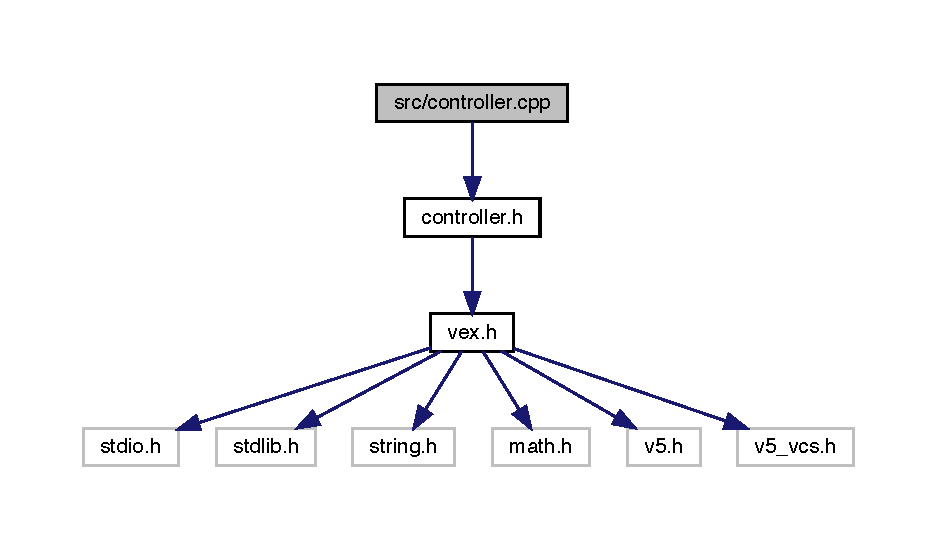
\includegraphics[width=350pt]{d6/d7c/controller_8cpp__incl}
\end{center}
\end{figure}
\doxysubsection*{Functions}
\begin{DoxyCompactItemize}
\item 
int \mbox{\hyperlink{controller_8cpp_a73be3a8649e7d561a68cd816420efbd9_a73be3a8649e7d561a68cd816420efbd9}{axis\+Value}} (controller\+::axis Axis)
\item 
bool \mbox{\hyperlink{controller_8cpp_aff3b02388de758f0fe6d98930ea57626_aff3b02388de758f0fe6d98930ea57626}{button\+Is\+Pressed}} (controller\+::button Button)
\end{DoxyCompactItemize}


\doxysubsection{Function Documentation}
\mbox{\Hypertarget{controller_8cpp_a73be3a8649e7d561a68cd816420efbd9_a73be3a8649e7d561a68cd816420efbd9}\label{controller_8cpp_a73be3a8649e7d561a68cd816420efbd9_a73be3a8649e7d561a68cd816420efbd9}} 
\index{controller.cpp@{controller.cpp}!axisValue@{axisValue}}
\index{axisValue@{axisValue}!controller.cpp@{controller.cpp}}
\doxysubsubsection{\texorpdfstring{axisValue()}{axisValue()}}
{\footnotesize\ttfamily int axis\+Value (\begin{DoxyParamCaption}\item[{controller\+::axis}]{Axis }\end{DoxyParamCaption})}

Returns an axis value of the controller in a -\/100 -\/ 100 scale, designed to be used with motor speeds in percent 
\begin{DoxyParams}{Parameters}
{\em Axis} & the axis on the controller that will be read (Ex. \mbox{[}controller\mbox{]}.axis3 for the left x axis) \\
\hline
\end{DoxyParams}
\begin{DoxyAuthor}{Author}
Michael Baraty 
\end{DoxyAuthor}
\begin{DoxyDate}{Date}
11/9/2019 
\end{DoxyDate}


Definition at line \mbox{\hyperlink{controller_8cpp_source_l00004}{4}} of file \mbox{\hyperlink{controller_8cpp_source}{controller.\+cpp}}.


\begin{DoxyCode}{0}
\DoxyCodeLine{00004                                    \{}
\DoxyCodeLine{00005   \textcolor{keywordflow}{return} Axis.position();}
\DoxyCodeLine{00006 \}}

\end{DoxyCode}
Here is the caller graph for this function\+:\nopagebreak
\begin{figure}[H]
\begin{center}
\leavevmode
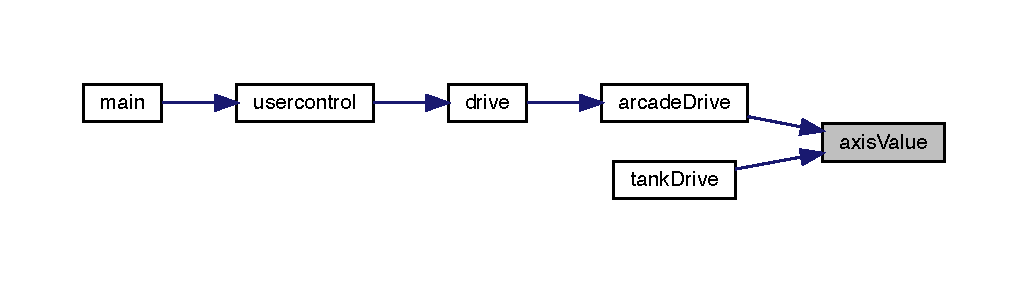
\includegraphics[width=350pt]{d1/d47/controller_8cpp_a73be3a8649e7d561a68cd816420efbd9_a73be3a8649e7d561a68cd816420efbd9_icgraph}
\end{center}
\end{figure}
\mbox{\Hypertarget{controller_8cpp_aff3b02388de758f0fe6d98930ea57626_aff3b02388de758f0fe6d98930ea57626}\label{controller_8cpp_aff3b02388de758f0fe6d98930ea57626_aff3b02388de758f0fe6d98930ea57626}} 
\index{controller.cpp@{controller.cpp}!buttonIsPressed@{buttonIsPressed}}
\index{buttonIsPressed@{buttonIsPressed}!controller.cpp@{controller.cpp}}
\doxysubsubsection{\texorpdfstring{buttonIsPressed()}{buttonIsPressed()}}
{\footnotesize\ttfamily bool button\+Is\+Pressed (\begin{DoxyParamCaption}\item[{controller\+::button}]{Button }\end{DoxyParamCaption})}

Returns a boolean for whether a designated button is being pressed 
\begin{DoxyParams}{Parameters}
{\em Button} & the button on the controller that will be read (Ex. \mbox{[}controller\mbox{]}.buttonA for the A button) \\
\hline
\end{DoxyParams}
\begin{DoxyAuthor}{Author}
Michael Baraty 
\end{DoxyAuthor}
\begin{DoxyDate}{Date}
11/9/2019 
\end{DoxyDate}


Definition at line \mbox{\hyperlink{controller_8cpp_source_l00008}{8}} of file \mbox{\hyperlink{controller_8cpp_source}{controller.\+cpp}}.


\begin{DoxyCode}{0}
\DoxyCodeLine{00008                                               \{}
\DoxyCodeLine{00009   \textcolor{keywordflow}{return} Button.pressing();}
\DoxyCodeLine{00010 \}}

\end{DoxyCode}
Here is the caller graph for this function\+:\nopagebreak
\begin{figure}[H]
\begin{center}
\leavevmode
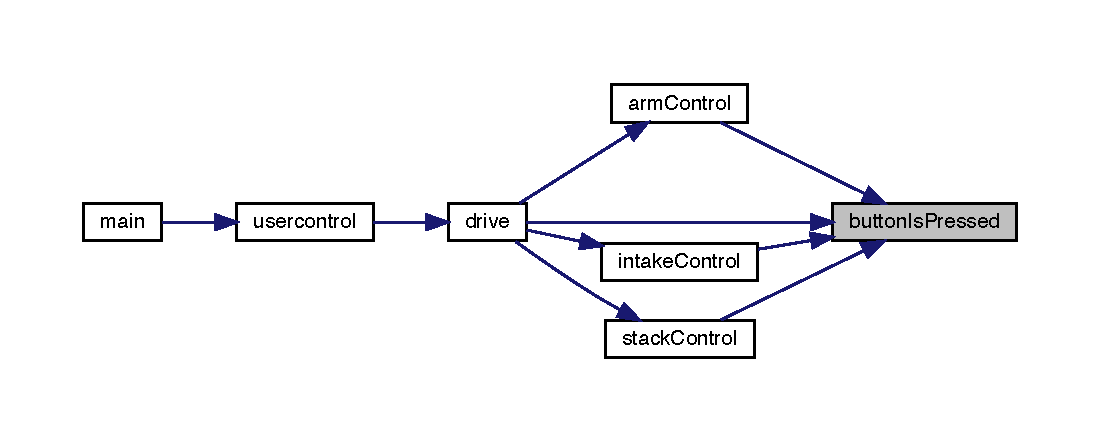
\includegraphics[width=350pt]{d1/d47/controller_8cpp_aff3b02388de758f0fe6d98930ea57626_aff3b02388de758f0fe6d98930ea57626_icgraph}
\end{center}
\end{figure}

\hypertarget{controller_8cpp_source}{}\subsection{controller.\+cpp}
\label{controller_8cpp_source}\index{src/controller.\+cpp@{src/controller.\+cpp}}

\begin{DoxyCode}
00001 \textcolor{preprocessor}{#include "\mbox{\hyperlink{controller_8h}{controller.h}}"}
00002 
00003 
\Hypertarget{controller_8cpp_source_l00004}\mbox{\hyperlink{controller_8cpp_a73be3a8649e7d561a68cd816420efbd9_a73be3a8649e7d561a68cd816420efbd9}{00004}} \textcolor{keywordtype}{int} \mbox{\hyperlink{controller_8cpp_a73be3a8649e7d561a68cd816420efbd9_a73be3a8649e7d561a68cd816420efbd9}{axisValue}}(controller::axis Axis) \{
00005   \textcolor{keywordflow}{return} Axis.position();
00006 \}
00007 
\Hypertarget{controller_8cpp_source_l00008}\mbox{\hyperlink{controller_8cpp_aff3b02388de758f0fe6d98930ea57626_aff3b02388de758f0fe6d98930ea57626}{00008}} \textcolor{keywordtype}{bool} \mbox{\hyperlink{controller_8cpp_aff3b02388de758f0fe6d98930ea57626_aff3b02388de758f0fe6d98930ea57626}{buttonIsPressed}}(controller::button Button) \{
00009   \textcolor{keywordflow}{return} Button.pressing();
00010 \}
00011 
00012 
00013 
00014 
00015  
\end{DoxyCode}

\hypertarget{drive_8cpp}{}\doxysection{src/drive.cpp File Reference}
\label{drive_8cpp}\index{src/drive.cpp@{src/drive.cpp}}
{\ttfamily \#include \char`\"{}drive.\+h\char`\"{}}\newline
{\ttfamily \#include \char`\"{}declarations.\+h\char`\"{}}\newline
{\ttfamily \#include \char`\"{}auton.\+h\char`\"{}}\newline
Include dependency graph for drive.\+cpp\+:\nopagebreak
\begin{figure}[H]
\begin{center}
\leavevmode
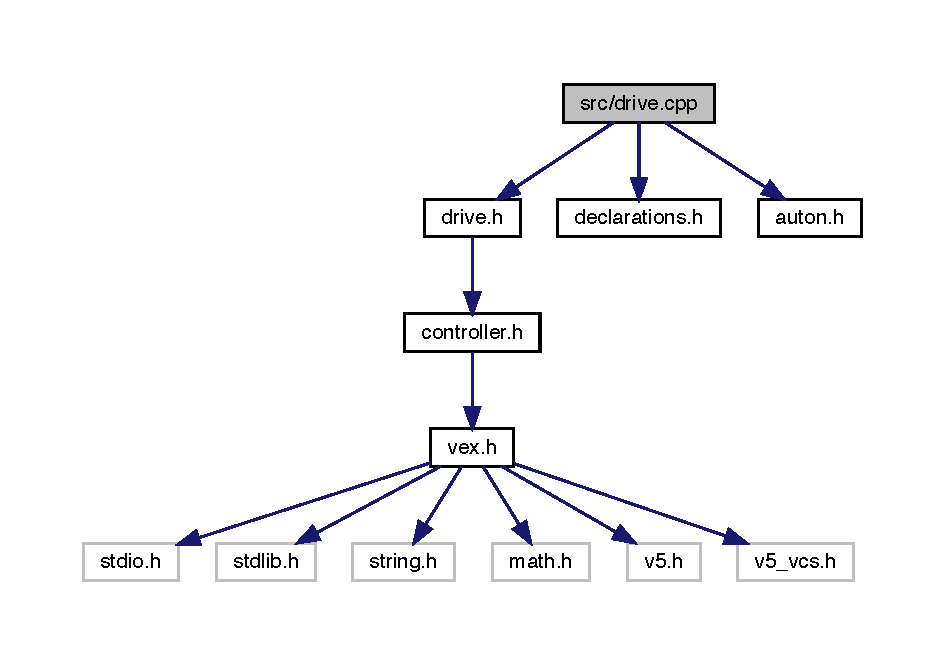
\includegraphics[width=350pt]{db/ddd/drive_8cpp__incl}
\end{center}
\end{figure}
\doxysubsection*{Functions}
\begin{DoxyCompactItemize}
\item 
void \mbox{\hyperlink{drive_8cpp_a928e32686c7e00c1ecde24c3da3019f7_a928e32686c7e00c1ecde24c3da3019f7}{drive}} ()
\item 
void \mbox{\hyperlink{drive_8cpp_ac522da2148fe1cfd9bea8c026e64ee7b_ac522da2148fe1cfd9bea8c026e64ee7b}{set\+Side\+Speed}} (\mbox{\hyperlink{drive_8h_a2771dd4b083c12b0f13d534e3d1914dc_a2771dd4b083c12b0f13d534e3d1914dc}{Drive\+Side}} side, int speed)
\item 
void \mbox{\hyperlink{drive_8cpp_a6ff8820b82f28a73c88a746ddacb26bb_a6ff8820b82f28a73c88a746ddacb26bb}{arcade\+Drive}} ()
\item 
void \mbox{\hyperlink{drive_8cpp_ab8605578ac6dddeb3e511513523e3354_ab8605578ac6dddeb3e511513523e3354}{tank\+Drive}} ()
\item 
void \mbox{\hyperlink{drive_8cpp_a08a55986dab46203f1eeef50123cf4bd_a08a55986dab46203f1eeef50123cf4bd}{move\+Stack\+Forward}} ()
\item 
void \mbox{\hyperlink{drive_8cpp_ac153148440cec552a2824c91569e1e5a_ac153148440cec552a2824c91569e1e5a}{move\+Stack\+Back}} ()
\item 
void \mbox{\hyperlink{drive_8cpp_abc3819041cf96aad1093752a3a5de31c_abc3819041cf96aad1093752a3a5de31c}{stack\+Control}} ()
\item 
void \mbox{\hyperlink{drive_8cpp_adf7b0afb3a8dcf884db533b0217b0543_adf7b0afb3a8dcf884db533b0217b0543}{arm\+Up}} ()
\item 
void \mbox{\hyperlink{drive_8cpp_ab1850cc7cdb69057fe29f45eefe7ec90_ab1850cc7cdb69057fe29f45eefe7ec90}{arm\+Down}} ()
\item 
void \mbox{\hyperlink{drive_8cpp_adde1067b42b4de65ff20afb8901f7643_adde1067b42b4de65ff20afb8901f7643}{arm\+Control}} ()
\item 
void \mbox{\hyperlink{drive_8cpp_aa0846c73538fc48569a7c7c3689a59f0_aa0846c73538fc48569a7c7c3689a59f0}{intake\+In}} ()
\item 
void \mbox{\hyperlink{drive_8cpp_aaca1ffa87592c1c5783fe6e18f9c655b_aaca1ffa87592c1c5783fe6e18f9c655b}{intake\+Out}} ()
\item 
void \mbox{\hyperlink{drive_8cpp_a8afb2a071b21d98c49d5888a7b380ba6_a8afb2a071b21d98c49d5888a7b380ba6}{intake\+Control}} ()
\end{DoxyCompactItemize}
\doxysubsection*{Variables}
\begin{DoxyCompactItemize}
\item 
bool \mbox{\hyperlink{drive_8cpp_ac84adc1c8ccd21c3c630031ad1ce5956_ac84adc1c8ccd21c3c630031ad1ce5956}{slow\+Mode}} = false
\end{DoxyCompactItemize}


\doxysubsection{Function Documentation}
\mbox{\Hypertarget{drive_8cpp_a6ff8820b82f28a73c88a746ddacb26bb_a6ff8820b82f28a73c88a746ddacb26bb}\label{drive_8cpp_a6ff8820b82f28a73c88a746ddacb26bb_a6ff8820b82f28a73c88a746ddacb26bb}} 
\index{drive.cpp@{drive.cpp}!arcadeDrive@{arcadeDrive}}
\index{arcadeDrive@{arcadeDrive}!drive.cpp@{drive.cpp}}
\doxysubsubsection{\texorpdfstring{arcadeDrive()}{arcadeDrive()}}
{\footnotesize\ttfamily void arcade\+Drive (\begin{DoxyParamCaption}{ }\end{DoxyParamCaption})}

Initiates the arcade control configuration for the controller, with the left y axis for linear movement and the right x axis for pivoting \begin{DoxyAuthor}{Author}
Michael Baraty 
\end{DoxyAuthor}
\begin{DoxyDate}{Date}
11/9/2019 
\end{DoxyDate}


Definition at line \mbox{\hyperlink{drive_8cpp_source_l00037}{37}} of file \mbox{\hyperlink{drive_8cpp_source}{drive.\+cpp}}.


\begin{DoxyCode}{0}
\DoxyCodeLine{00037                    \{}
\DoxyCodeLine{00038   \textcolor{keywordtype}{int} x = \mbox{\hyperlink{declarations_8h_afb49f22bdd1e93218d02bb25e513e8a0_afb49f22bdd1e93218d02bb25e513e8a0}{SPEED\_MULTIPLIER}}  * -\/\mbox{\hyperlink{controller_8h_a73be3a8649e7d561a68cd816420efbd9_a73be3a8649e7d561a68cd816420efbd9}{axisValue}}(\mbox{\hyperlink{declarations_8h_ab04f8ff803f7f02c23e713402e13bf32_ab04f8ff803f7f02c23e713402e13bf32}{MASTER}}.Axis1);}
\DoxyCodeLine{00039   \textcolor{keywordtype}{int} y = \mbox{\hyperlink{declarations_8h_afb49f22bdd1e93218d02bb25e513e8a0_afb49f22bdd1e93218d02bb25e513e8a0}{SPEED\_MULTIPLIER}} * (.7  * (pow(-\/\mbox{\hyperlink{controller_8h_a73be3a8649e7d561a68cd816420efbd9_a73be3a8649e7d561a68cd816420efbd9}{axisValue}}(\mbox{\hyperlink{declarations_8h_ab04f8ff803f7f02c23e713402e13bf32_ab04f8ff803f7f02c23e713402e13bf32}{MASTER}}.Axis3) / 9, 3) / 10));}
\DoxyCodeLine{00040   \textcolor{keywordtype}{int} speedLeft = abs(x + y) > \mbox{\hyperlink{declarations_8h_adceb947873623dd2a87f7f69e81fbd38_adceb947873623dd2a87f7f69e81fbd38}{THRESHOLD}}? -\/(x + y): 0;}
\DoxyCodeLine{00041   \textcolor{keywordtype}{int} speedRight = abs(x -\/ y) > \mbox{\hyperlink{declarations_8h_adceb947873623dd2a87f7f69e81fbd38_adceb947873623dd2a87f7f69e81fbd38}{THRESHOLD}}? (x -\/ y): 0;}
\DoxyCodeLine{00042 }
\DoxyCodeLine{00043   \textcolor{keywordflow}{if}(\mbox{\hyperlink{drive_8cpp_ac84adc1c8ccd21c3c630031ad1ce5956_ac84adc1c8ccd21c3c630031ad1ce5956}{slowMode}})\{}
\DoxyCodeLine{00044     \mbox{\hyperlink{drive_8cpp_ac522da2148fe1cfd9bea8c026e64ee7b_ac522da2148fe1cfd9bea8c026e64ee7b}{setSideSpeed}}(\mbox{\hyperlink{drive_8h_a2771dd4b083c12b0f13d534e3d1914dc_a2771dd4b083c12b0f13d534e3d1914dca684d325a7303f52e64011467ff5c5758}{DriveSide::LEFT}}, speedLeft / 3);}
\DoxyCodeLine{00045      \mbox{\hyperlink{drive_8cpp_ac522da2148fe1cfd9bea8c026e64ee7b_ac522da2148fe1cfd9bea8c026e64ee7b}{setSideSpeed}}(\mbox{\hyperlink{drive_8h_a2771dd4b083c12b0f13d534e3d1914dc_a2771dd4b083c12b0f13d534e3d1914dca21507b40c80068eda19865706fdc2403}{DriveSide::RIGHT}}, speedRight / 3);}
\DoxyCodeLine{00046   \} \textcolor{keywordflow}{else} \{}
\DoxyCodeLine{00047     \mbox{\hyperlink{drive_8cpp_ac522da2148fe1cfd9bea8c026e64ee7b_ac522da2148fe1cfd9bea8c026e64ee7b}{setSideSpeed}}(\mbox{\hyperlink{drive_8h_a2771dd4b083c12b0f13d534e3d1914dc_a2771dd4b083c12b0f13d534e3d1914dca684d325a7303f52e64011467ff5c5758}{DriveSide::LEFT}}, speedLeft);}
\DoxyCodeLine{00048     \mbox{\hyperlink{drive_8cpp_ac522da2148fe1cfd9bea8c026e64ee7b_ac522da2148fe1cfd9bea8c026e64ee7b}{setSideSpeed}}(\mbox{\hyperlink{drive_8h_a2771dd4b083c12b0f13d534e3d1914dc_a2771dd4b083c12b0f13d534e3d1914dca21507b40c80068eda19865706fdc2403}{DriveSide::RIGHT}}, speedRight);}
\DoxyCodeLine{00049   \}}
\DoxyCodeLine{00050 \}}

\end{DoxyCode}
Here is the call graph for this function\+:\nopagebreak
\begin{figure}[H]
\begin{center}
\leavevmode
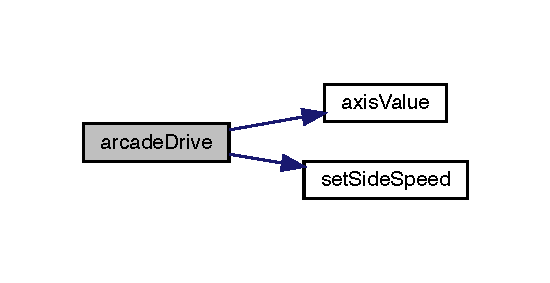
\includegraphics[width=264pt]{de/de5/drive_8cpp_a6ff8820b82f28a73c88a746ddacb26bb_a6ff8820b82f28a73c88a746ddacb26bb_cgraph}
\end{center}
\end{figure}
Here is the caller graph for this function\+:\nopagebreak
\begin{figure}[H]
\begin{center}
\leavevmode
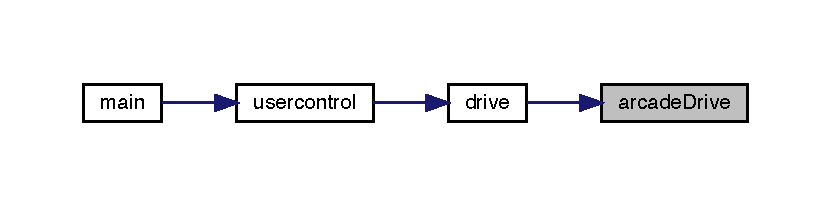
\includegraphics[width=350pt]{de/de5/drive_8cpp_a6ff8820b82f28a73c88a746ddacb26bb_a6ff8820b82f28a73c88a746ddacb26bb_icgraph}
\end{center}
\end{figure}
\mbox{\Hypertarget{drive_8cpp_adde1067b42b4de65ff20afb8901f7643_adde1067b42b4de65ff20afb8901f7643}\label{drive_8cpp_adde1067b42b4de65ff20afb8901f7643_adde1067b42b4de65ff20afb8901f7643}} 
\index{drive.cpp@{drive.cpp}!armControl@{armControl}}
\index{armControl@{armControl}!drive.cpp@{drive.cpp}}
\doxysubsubsection{\texorpdfstring{armControl()}{armControl()}}
{\footnotesize\ttfamily void arm\+Control (\begin{DoxyParamCaption}{ }\end{DoxyParamCaption})}

Reads the controller\textquotesingle{}s button inputs to initiate the arm lifter\textquotesingle{}s movement while the button is being pressed \begin{DoxyAuthor}{Author}
Michael Baraty 
\end{DoxyAuthor}
\begin{DoxyDate}{Date}
11/9/2019 
\end{DoxyDate}


Definition at line \mbox{\hyperlink{drive_8cpp_source_l00097}{97}} of file \mbox{\hyperlink{drive_8cpp_source}{drive.\+cpp}}.


\begin{DoxyCode}{0}
\DoxyCodeLine{00097                  \{}
\DoxyCodeLine{00098   \textcolor{keywordflow}{if}(\mbox{\hyperlink{controller_8h_aff3b02388de758f0fe6d98930ea57626_aff3b02388de758f0fe6d98930ea57626}{buttonIsPressed}}(\mbox{\hyperlink{declarations_8h_ab04f8ff803f7f02c23e713402e13bf32_ab04f8ff803f7f02c23e713402e13bf32}{MASTER}}.ButtonR1))\{}
\DoxyCodeLine{00099     \mbox{\hyperlink{drive_8cpp_adf7b0afb3a8dcf884db533b0217b0543_adf7b0afb3a8dcf884db533b0217b0543}{armUp}}();}
\DoxyCodeLine{00100   \}}
\DoxyCodeLine{00101   \textcolor{keywordflow}{else} \textcolor{keywordflow}{if} (\mbox{\hyperlink{controller_8h_aff3b02388de758f0fe6d98930ea57626_aff3b02388de758f0fe6d98930ea57626}{buttonIsPressed}}(\mbox{\hyperlink{declarations_8h_ab04f8ff803f7f02c23e713402e13bf32_ab04f8ff803f7f02c23e713402e13bf32}{MASTER}}.ButtonR2)) \{}
\DoxyCodeLine{00102     \mbox{\hyperlink{drive_8cpp_ab1850cc7cdb69057fe29f45eefe7ec90_ab1850cc7cdb69057fe29f45eefe7ec90}{armDown}}();}
\DoxyCodeLine{00103   \}}
\DoxyCodeLine{00104   \textcolor{keywordflow}{else} \{}
\DoxyCodeLine{00105     \mbox{\hyperlink{declarations_8h_a9a834f9a2c804ef0d65ed2f68c10a61a_a9a834f9a2c804ef0d65ed2f68c10a61a}{MOTOR\_ARM}}.stop(brakeType::hold);}
\DoxyCodeLine{00106   \}}
\DoxyCodeLine{00107 \}}

\end{DoxyCode}
Here is the call graph for this function\+:\nopagebreak
\begin{figure}[H]
\begin{center}
\leavevmode
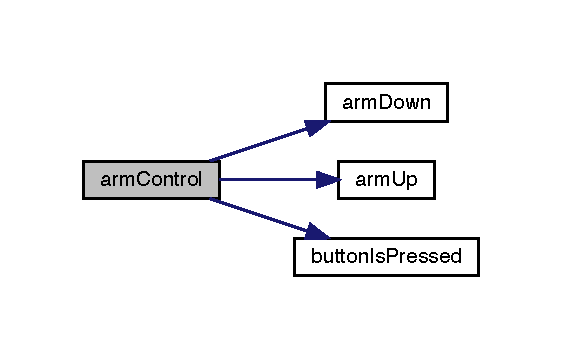
\includegraphics[width=270pt]{de/de5/drive_8cpp_adde1067b42b4de65ff20afb8901f7643_adde1067b42b4de65ff20afb8901f7643_cgraph}
\end{center}
\end{figure}
Here is the caller graph for this function\+:\nopagebreak
\begin{figure}[H]
\begin{center}
\leavevmode
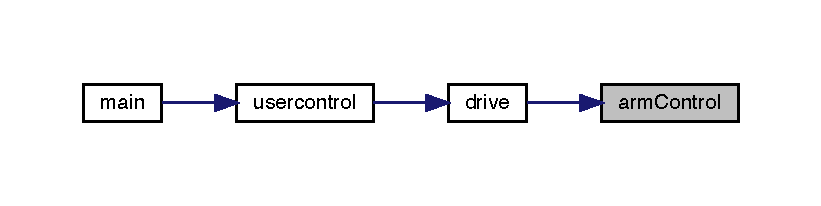
\includegraphics[width=350pt]{de/de5/drive_8cpp_adde1067b42b4de65ff20afb8901f7643_adde1067b42b4de65ff20afb8901f7643_icgraph}
\end{center}
\end{figure}
\mbox{\Hypertarget{drive_8cpp_ab1850cc7cdb69057fe29f45eefe7ec90_ab1850cc7cdb69057fe29f45eefe7ec90}\label{drive_8cpp_ab1850cc7cdb69057fe29f45eefe7ec90_ab1850cc7cdb69057fe29f45eefe7ec90}} 
\index{drive.cpp@{drive.cpp}!armDown@{armDown}}
\index{armDown@{armDown}!drive.cpp@{drive.cpp}}
\doxysubsubsection{\texorpdfstring{armDown()}{armDown()}}
{\footnotesize\ttfamily void arm\+Down (\begin{DoxyParamCaption}{ }\end{DoxyParamCaption})}

Moves the intake lifter down to a specified position \begin{DoxyAuthor}{Author}
Michael Baraty 
\end{DoxyAuthor}
\begin{DoxyDate}{Date}
11/9/2019 
\end{DoxyDate}


Definition at line \mbox{\hyperlink{drive_8cpp_source_l00092}{92}} of file \mbox{\hyperlink{drive_8cpp_source}{drive.\+cpp}}.


\begin{DoxyCode}{0}
\DoxyCodeLine{00092               \{}
\DoxyCodeLine{00093   \mbox{\hyperlink{declarations_8h_a9a834f9a2c804ef0d65ed2f68c10a61a_a9a834f9a2c804ef0d65ed2f68c10a61a}{MOTOR\_ARM}}.startSpinTo(-\/10, rotationUnits::rev, 100, velocityUnits::pct);}
\DoxyCodeLine{00094   \textcolor{comment}{//realValue 0}}
\DoxyCodeLine{00095 \}}

\end{DoxyCode}
Here is the caller graph for this function\+:\nopagebreak
\begin{figure}[H]
\begin{center}
\leavevmode
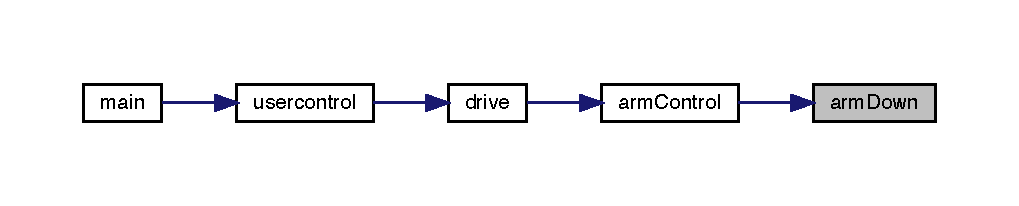
\includegraphics[width=350pt]{de/de5/drive_8cpp_ab1850cc7cdb69057fe29f45eefe7ec90_ab1850cc7cdb69057fe29f45eefe7ec90_icgraph}
\end{center}
\end{figure}
\mbox{\Hypertarget{drive_8cpp_adf7b0afb3a8dcf884db533b0217b0543_adf7b0afb3a8dcf884db533b0217b0543}\label{drive_8cpp_adf7b0afb3a8dcf884db533b0217b0543_adf7b0afb3a8dcf884db533b0217b0543}} 
\index{drive.cpp@{drive.cpp}!armUp@{armUp}}
\index{armUp@{armUp}!drive.cpp@{drive.cpp}}
\doxysubsubsection{\texorpdfstring{armUp()}{armUp()}}
{\footnotesize\ttfamily void arm\+Up (\begin{DoxyParamCaption}{ }\end{DoxyParamCaption})}

Moves the intake lifter up to a specified position \begin{DoxyAuthor}{Author}
Michael Baraty 
\end{DoxyAuthor}
\begin{DoxyDate}{Date}
11/9/2019 
\end{DoxyDate}


Definition at line \mbox{\hyperlink{drive_8cpp_source_l00087}{87}} of file \mbox{\hyperlink{drive_8cpp_source}{drive.\+cpp}}.


\begin{DoxyCode}{0}
\DoxyCodeLine{00087             \{}
\DoxyCodeLine{00088   \mbox{\hyperlink{declarations_8h_a9a834f9a2c804ef0d65ed2f68c10a61a_a9a834f9a2c804ef0d65ed2f68c10a61a}{MOTOR\_ARM}}.startSpinTo(60.6, rotationUnits::rev, 100, velocityUnits::pct);}
\DoxyCodeLine{00089   \textcolor{comment}{//realValue 6.6}}
\DoxyCodeLine{00090 \}}

\end{DoxyCode}
Here is the caller graph for this function\+:\nopagebreak
\begin{figure}[H]
\begin{center}
\leavevmode
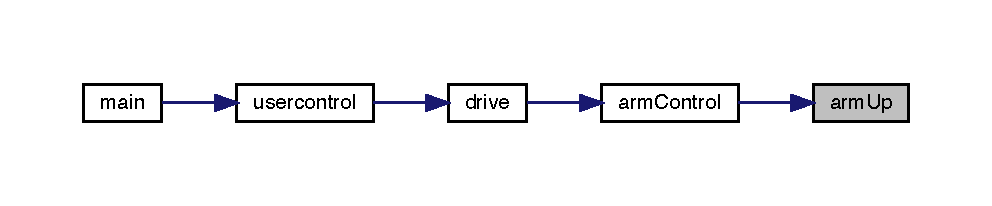
\includegraphics[width=350pt]{de/de5/drive_8cpp_adf7b0afb3a8dcf884db533b0217b0543_adf7b0afb3a8dcf884db533b0217b0543_icgraph}
\end{center}
\end{figure}
\mbox{\Hypertarget{drive_8cpp_a928e32686c7e00c1ecde24c3da3019f7_a928e32686c7e00c1ecde24c3da3019f7}\label{drive_8cpp_a928e32686c7e00c1ecde24c3da3019f7_a928e32686c7e00c1ecde24c3da3019f7}} 
\index{drive.cpp@{drive.cpp}!drive@{drive}}
\index{drive@{drive}!drive.cpp@{drive.cpp}}
\doxysubsubsection{\texorpdfstring{drive()}{drive()}}
{\footnotesize\ttfamily void drive (\begin{DoxyParamCaption}{ }\end{DoxyParamCaption})}

Initiates the drive code for the entire robot \begin{DoxyAuthor}{Author}
Michael Baraty 
\end{DoxyAuthor}
\begin{DoxyDate}{Date}
11/9/2019 
\end{DoxyDate}


Definition at line \mbox{\hyperlink{drive_8cpp_source_l00007}{7}} of file \mbox{\hyperlink{drive_8cpp_source}{drive.\+cpp}}.


\begin{DoxyCode}{0}
\DoxyCodeLine{00007              \{}
\DoxyCodeLine{00008   \mbox{\hyperlink{drive_8cpp_a6ff8820b82f28a73c88a746ddacb26bb_a6ff8820b82f28a73c88a746ddacb26bb}{arcadeDrive}}();}
\DoxyCodeLine{00009   \mbox{\hyperlink{drive_8cpp_abc3819041cf96aad1093752a3a5de31c_abc3819041cf96aad1093752a3a5de31c}{stackControl}}();}
\DoxyCodeLine{00010   \mbox{\hyperlink{drive_8cpp_adde1067b42b4de65ff20afb8901f7643_adde1067b42b4de65ff20afb8901f7643}{armControl}}();}
\DoxyCodeLine{00011   \mbox{\hyperlink{drive_8cpp_a8afb2a071b21d98c49d5888a7b380ba6_a8afb2a071b21d98c49d5888a7b380ba6}{intakeControl}}();}
\DoxyCodeLine{00012 }
\DoxyCodeLine{00013   \textcolor{keywordflow}{if}(\mbox{\hyperlink{controller_8h_aff3b02388de758f0fe6d98930ea57626_aff3b02388de758f0fe6d98930ea57626}{buttonIsPressed}}(\mbox{\hyperlink{declarations_8h_ab04f8ff803f7f02c23e713402e13bf32_ab04f8ff803f7f02c23e713402e13bf32}{MASTER}}.ButtonUp))\{}
\DoxyCodeLine{00014     \mbox{\hyperlink{drive_8cpp_ac84adc1c8ccd21c3c630031ad1ce5956_ac84adc1c8ccd21c3c630031ad1ce5956}{slowMode}} = \textcolor{keyword}{false};}
\DoxyCodeLine{00015   \} \textcolor{keywordflow}{else} \textcolor{keywordflow}{if}(\mbox{\hyperlink{controller_8h_aff3b02388de758f0fe6d98930ea57626_aff3b02388de758f0fe6d98930ea57626}{buttonIsPressed}}(\mbox{\hyperlink{declarations_8h_ab04f8ff803f7f02c23e713402e13bf32_ab04f8ff803f7f02c23e713402e13bf32}{MASTER}}.ButtonDown))\{}
\DoxyCodeLine{00016     \mbox{\hyperlink{drive_8cpp_ac84adc1c8ccd21c3c630031ad1ce5956_ac84adc1c8ccd21c3c630031ad1ce5956}{slowMode}} = \textcolor{keyword}{true};}
\DoxyCodeLine{00017   \}}
\DoxyCodeLine{00018 }
\DoxyCodeLine{00019 \}}

\end{DoxyCode}
Here is the call graph for this function\+:\nopagebreak
\begin{figure}[H]
\begin{center}
\leavevmode
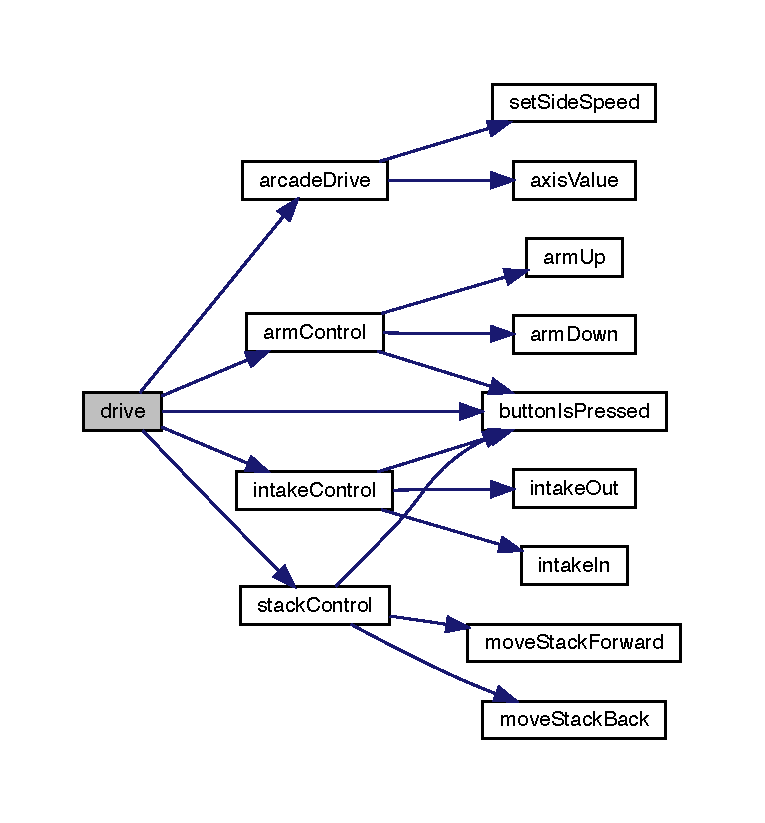
\includegraphics[width=350pt]{de/de5/drive_8cpp_a928e32686c7e00c1ecde24c3da3019f7_a928e32686c7e00c1ecde24c3da3019f7_cgraph}
\end{center}
\end{figure}
Here is the caller graph for this function\+:\nopagebreak
\begin{figure}[H]
\begin{center}
\leavevmode
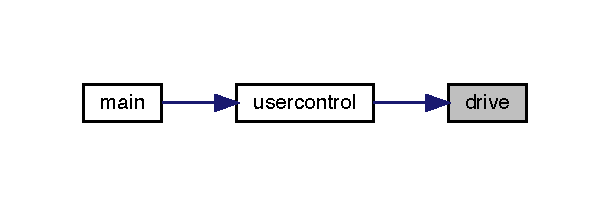
\includegraphics[width=293pt]{de/de5/drive_8cpp_a928e32686c7e00c1ecde24c3da3019f7_a928e32686c7e00c1ecde24c3da3019f7_icgraph}
\end{center}
\end{figure}
\mbox{\Hypertarget{drive_8cpp_a8afb2a071b21d98c49d5888a7b380ba6_a8afb2a071b21d98c49d5888a7b380ba6}\label{drive_8cpp_a8afb2a071b21d98c49d5888a7b380ba6_a8afb2a071b21d98c49d5888a7b380ba6}} 
\index{drive.cpp@{drive.cpp}!intakeControl@{intakeControl}}
\index{intakeControl@{intakeControl}!drive.cpp@{drive.cpp}}
\doxysubsubsection{\texorpdfstring{intakeControl()}{intakeControl()}}
{\footnotesize\ttfamily void intake\+Control (\begin{DoxyParamCaption}{ }\end{DoxyParamCaption})}

Reads the controller\textquotesingle{}s button inputs to spin the intake while the button is being pressed \begin{DoxyAuthor}{Author}
Michael Baraty 
\end{DoxyAuthor}
\begin{DoxyDate}{Date}
11/9/2019 
\end{DoxyDate}


Definition at line \mbox{\hyperlink{drive_8cpp_source_l00129}{129}} of file \mbox{\hyperlink{drive_8cpp_source}{drive.\+cpp}}.


\begin{DoxyCode}{0}
\DoxyCodeLine{00129                      \{}
\DoxyCodeLine{00130   \textcolor{keywordflow}{if}(\mbox{\hyperlink{controller_8h_aff3b02388de758f0fe6d98930ea57626_aff3b02388de758f0fe6d98930ea57626}{buttonIsPressed}}(\mbox{\hyperlink{declarations_8h_ab04f8ff803f7f02c23e713402e13bf32_ab04f8ff803f7f02c23e713402e13bf32}{MASTER}}.ButtonL1))\{}
\DoxyCodeLine{00131     \mbox{\hyperlink{drive_8cpp_aa0846c73538fc48569a7c7c3689a59f0_aa0846c73538fc48569a7c7c3689a59f0}{intakeIn}}();}
\DoxyCodeLine{00132   \}}
\DoxyCodeLine{00133   \textcolor{keywordflow}{else} \textcolor{keywordflow}{if} (\mbox{\hyperlink{controller_8h_aff3b02388de758f0fe6d98930ea57626_aff3b02388de758f0fe6d98930ea57626}{buttonIsPressed}}(\mbox{\hyperlink{declarations_8h_ab04f8ff803f7f02c23e713402e13bf32_ab04f8ff803f7f02c23e713402e13bf32}{MASTER}}.ButtonL2)) \{}
\DoxyCodeLine{00134     \mbox{\hyperlink{drive_8cpp_aaca1ffa87592c1c5783fe6e18f9c655b_aaca1ffa87592c1c5783fe6e18f9c655b}{intakeOut}}();}
\DoxyCodeLine{00135   \}}
\DoxyCodeLine{00136   \textcolor{keywordflow}{else} \{}
\DoxyCodeLine{00137     \mbox{\hyperlink{declarations_8h_a34de211d15bfb3c0ac450597fd96b4fc_a34de211d15bfb3c0ac450597fd96b4fc}{MOTOR\_INTAKE\_A}}.stop(brakeType::hold);}
\DoxyCodeLine{00138     \mbox{\hyperlink{declarations_8h_a5ae79e7ed71b0b94b3983c22c60c2eaa_a5ae79e7ed71b0b94b3983c22c60c2eaa}{MOTOR\_INTAKE\_B}}.stop(brakeType::hold);}
\DoxyCodeLine{00139   \}}
\DoxyCodeLine{00140 \}}

\end{DoxyCode}
Here is the call graph for this function\+:\nopagebreak
\begin{figure}[H]
\begin{center}
\leavevmode
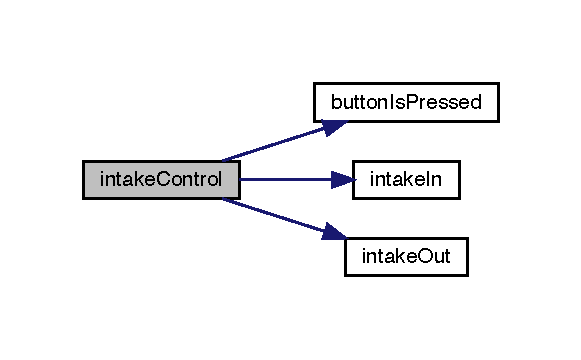
\includegraphics[width=279pt]{de/de5/drive_8cpp_a8afb2a071b21d98c49d5888a7b380ba6_a8afb2a071b21d98c49d5888a7b380ba6_cgraph}
\end{center}
\end{figure}
Here is the caller graph for this function\+:\nopagebreak
\begin{figure}[H]
\begin{center}
\leavevmode
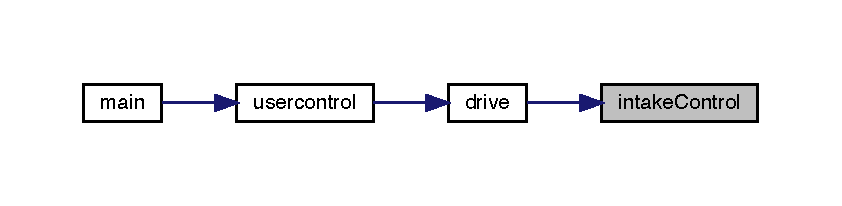
\includegraphics[width=350pt]{de/de5/drive_8cpp_a8afb2a071b21d98c49d5888a7b380ba6_a8afb2a071b21d98c49d5888a7b380ba6_icgraph}
\end{center}
\end{figure}
\mbox{\Hypertarget{drive_8cpp_aa0846c73538fc48569a7c7c3689a59f0_aa0846c73538fc48569a7c7c3689a59f0}\label{drive_8cpp_aa0846c73538fc48569a7c7c3689a59f0_aa0846c73538fc48569a7c7c3689a59f0}} 
\index{drive.cpp@{drive.cpp}!intakeIn@{intakeIn}}
\index{intakeIn@{intakeIn}!drive.cpp@{drive.cpp}}
\doxysubsubsection{\texorpdfstring{intakeIn()}{intakeIn()}}
{\footnotesize\ttfamily void intake\+In (\begin{DoxyParamCaption}{ }\end{DoxyParamCaption})}

Spins the intake to intake the cubes \begin{DoxyAuthor}{Author}
Michael Baraty 
\end{DoxyAuthor}
\begin{DoxyDate}{Date}
11/9/2019 
\end{DoxyDate}


Definition at line \mbox{\hyperlink{drive_8cpp_source_l00109}{109}} of file \mbox{\hyperlink{drive_8cpp_source}{drive.\+cpp}}.


\begin{DoxyCode}{0}
\DoxyCodeLine{00109                 \{}
\DoxyCodeLine{00110   \textcolor{keywordflow}{if}(!\mbox{\hyperlink{drive_8cpp_ac84adc1c8ccd21c3c630031ad1ce5956_ac84adc1c8ccd21c3c630031ad1ce5956}{slowMode}}) \{}
\DoxyCodeLine{00111     \mbox{\hyperlink{declarations_8h_a34de211d15bfb3c0ac450597fd96b4fc_a34de211d15bfb3c0ac450597fd96b4fc}{MOTOR\_INTAKE\_A}}.spin(directionType::fwd, 100, velocityUnits::pct);}
\DoxyCodeLine{00112     \mbox{\hyperlink{declarations_8h_a5ae79e7ed71b0b94b3983c22c60c2eaa_a5ae79e7ed71b0b94b3983c22c60c2eaa}{MOTOR\_INTAKE\_B}}.spin(directionType::fwd, 100, velocityUnits::pct);}
\DoxyCodeLine{00113   \} \textcolor{keywordflow}{else} \{}
\DoxyCodeLine{00114     \mbox{\hyperlink{declarations_8h_a34de211d15bfb3c0ac450597fd96b4fc_a34de211d15bfb3c0ac450597fd96b4fc}{MOTOR\_INTAKE\_A}}.spin(directionType::fwd, (100), velocityUnits::pct);}
\DoxyCodeLine{00115     \mbox{\hyperlink{declarations_8h_a5ae79e7ed71b0b94b3983c22c60c2eaa_a5ae79e7ed71b0b94b3983c22c60c2eaa}{MOTOR\_INTAKE\_B}}.spin(directionType::fwd, (100), velocityUnits::pct);}
\DoxyCodeLine{00116   \}}
\DoxyCodeLine{00117 \}}

\end{DoxyCode}
Here is the caller graph for this function\+:\nopagebreak
\begin{figure}[H]
\begin{center}
\leavevmode
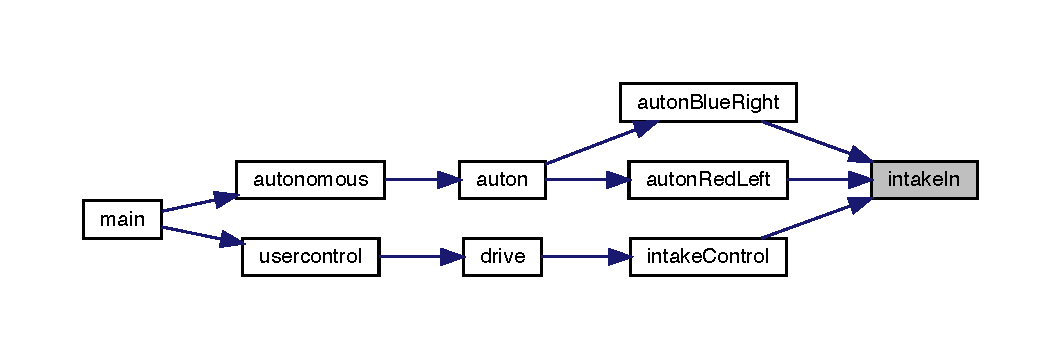
\includegraphics[width=350pt]{de/de5/drive_8cpp_aa0846c73538fc48569a7c7c3689a59f0_aa0846c73538fc48569a7c7c3689a59f0_icgraph}
\end{center}
\end{figure}
\mbox{\Hypertarget{drive_8cpp_aaca1ffa87592c1c5783fe6e18f9c655b_aaca1ffa87592c1c5783fe6e18f9c655b}\label{drive_8cpp_aaca1ffa87592c1c5783fe6e18f9c655b_aaca1ffa87592c1c5783fe6e18f9c655b}} 
\index{drive.cpp@{drive.cpp}!intakeOut@{intakeOut}}
\index{intakeOut@{intakeOut}!drive.cpp@{drive.cpp}}
\doxysubsubsection{\texorpdfstring{intakeOut()}{intakeOut()}}
{\footnotesize\ttfamily void intake\+Out (\begin{DoxyParamCaption}{ }\end{DoxyParamCaption})}

Spins the intake to eject the cubes \begin{DoxyAuthor}{Author}
Michael Baraty 
\end{DoxyAuthor}
\begin{DoxyDate}{Date}
11/9/2019 
\end{DoxyDate}


Definition at line \mbox{\hyperlink{drive_8cpp_source_l00119}{119}} of file \mbox{\hyperlink{drive_8cpp_source}{drive.\+cpp}}.


\begin{DoxyCode}{0}
\DoxyCodeLine{00119                  \{}
\DoxyCodeLine{00120    \textcolor{keywordflow}{if}(!\mbox{\hyperlink{drive_8cpp_ac84adc1c8ccd21c3c630031ad1ce5956_ac84adc1c8ccd21c3c630031ad1ce5956}{slowMode}}) \{}
\DoxyCodeLine{00121     \mbox{\hyperlink{declarations_8h_a34de211d15bfb3c0ac450597fd96b4fc_a34de211d15bfb3c0ac450597fd96b4fc}{MOTOR\_INTAKE\_A}}.spin(directionType::rev, 100, velocityUnits::pct);}
\DoxyCodeLine{00122     \mbox{\hyperlink{declarations_8h_a5ae79e7ed71b0b94b3983c22c60c2eaa_a5ae79e7ed71b0b94b3983c22c60c2eaa}{MOTOR\_INTAKE\_B}}.spin(directionType::rev, 100, velocityUnits::pct);}
\DoxyCodeLine{00123   \} \textcolor{keywordflow}{else} \{}
\DoxyCodeLine{00124     \mbox{\hyperlink{declarations_8h_a34de211d15bfb3c0ac450597fd96b4fc_a34de211d15bfb3c0ac450597fd96b4fc}{MOTOR\_INTAKE\_A}}.spin(directionType::rev, .5*(100), velocityUnits::pct);}
\DoxyCodeLine{00125     \mbox{\hyperlink{declarations_8h_a5ae79e7ed71b0b94b3983c22c60c2eaa_a5ae79e7ed71b0b94b3983c22c60c2eaa}{MOTOR\_INTAKE\_B}}.spin(directionType::rev, .5*(100), velocityUnits::pct);}
\DoxyCodeLine{00126   \}}
\DoxyCodeLine{00127 \}}

\end{DoxyCode}
Here is the caller graph for this function\+:\nopagebreak
\begin{figure}[H]
\begin{center}
\leavevmode
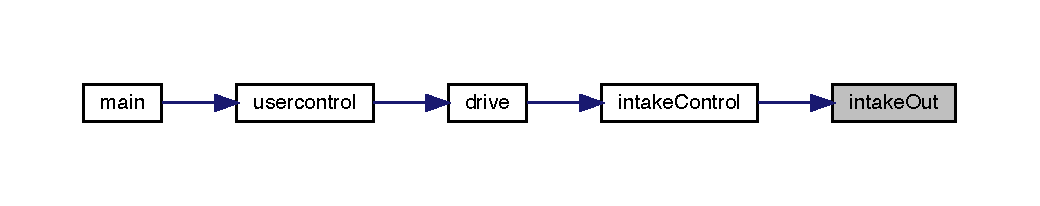
\includegraphics[width=350pt]{de/de5/drive_8cpp_aaca1ffa87592c1c5783fe6e18f9c655b_aaca1ffa87592c1c5783fe6e18f9c655b_icgraph}
\end{center}
\end{figure}
\mbox{\Hypertarget{drive_8cpp_ac153148440cec552a2824c91569e1e5a_ac153148440cec552a2824c91569e1e5a}\label{drive_8cpp_ac153148440cec552a2824c91569e1e5a_ac153148440cec552a2824c91569e1e5a}} 
\index{drive.cpp@{drive.cpp}!moveStackBack@{moveStackBack}}
\index{moveStackBack@{moveStackBack}!drive.cpp@{drive.cpp}}
\doxysubsubsection{\texorpdfstring{moveStackBack()}{moveStackBack()}}
{\footnotesize\ttfamily void move\+Stack\+Back (\begin{DoxyParamCaption}{ }\end{DoxyParamCaption})}

Moves the stack backwards to a specified position \begin{DoxyAuthor}{Author}
Michael Baraty 
\end{DoxyAuthor}
\begin{DoxyDate}{Date}
11/9/2019 
\end{DoxyDate}


Definition at line \mbox{\hyperlink{drive_8cpp_source_l00072}{72}} of file \mbox{\hyperlink{drive_8cpp_source}{drive.\+cpp}}.


\begin{DoxyCode}{0}
\DoxyCodeLine{00072                      \{}
\DoxyCodeLine{00073   \textcolor{keywordtype}{double} \textcolor{keyword}{final} = 0;}
\DoxyCodeLine{00074   \mbox{\hyperlink{declarations_8h_a212c888d64ffcd7e7b44a548fa0408a9_a212c888d64ffcd7e7b44a548fa0408a9}{MOTOR\_STACK}}.startSpinTo(-\/10, rotationUnits::rev, 80, velocityUnits::pct); }
\DoxyCodeLine{00075 \}}

\end{DoxyCode}
Here is the caller graph for this function\+:\nopagebreak
\begin{figure}[H]
\begin{center}
\leavevmode
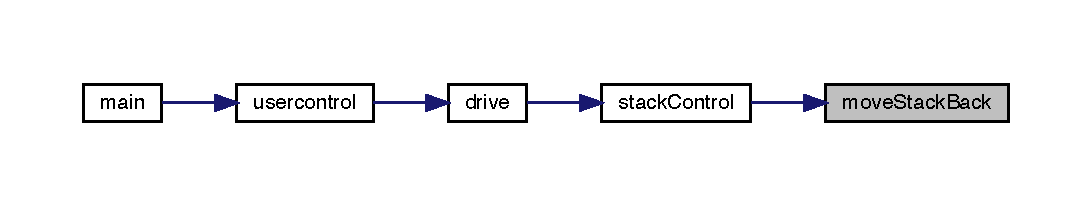
\includegraphics[width=350pt]{de/de5/drive_8cpp_ac153148440cec552a2824c91569e1e5a_ac153148440cec552a2824c91569e1e5a_icgraph}
\end{center}
\end{figure}
\mbox{\Hypertarget{drive_8cpp_a08a55986dab46203f1eeef50123cf4bd_a08a55986dab46203f1eeef50123cf4bd}\label{drive_8cpp_a08a55986dab46203f1eeef50123cf4bd_a08a55986dab46203f1eeef50123cf4bd}} 
\index{drive.cpp@{drive.cpp}!moveStackForward@{moveStackForward}}
\index{moveStackForward@{moveStackForward}!drive.cpp@{drive.cpp}}
\doxysubsubsection{\texorpdfstring{moveStackForward()}{moveStackForward()}}
{\footnotesize\ttfamily void move\+Stack\+Forward (\begin{DoxyParamCaption}{ }\end{DoxyParamCaption})}

Moves the stack forward to a specified position \begin{DoxyAuthor}{Author}
Michael Baraty 
\end{DoxyAuthor}
\begin{DoxyDate}{Date}
11/9/2019 
\end{DoxyDate}


Definition at line \mbox{\hyperlink{drive_8cpp_source_l00067}{67}} of file \mbox{\hyperlink{drive_8cpp_source}{drive.\+cpp}}.


\begin{DoxyCode}{0}
\DoxyCodeLine{00067                         \{}
\DoxyCodeLine{00068   \textcolor{keywordtype}{double} \textcolor{keyword}{final} = 1.5; }
\DoxyCodeLine{00069   \mbox{\hyperlink{declarations_8h_a212c888d64ffcd7e7b44a548fa0408a9_a212c888d64ffcd7e7b44a548fa0408a9}{MOTOR\_STACK}}.startSpinTo(10, rotationUnits::rev, 30, velocityUnits::pct);}
\DoxyCodeLine{00070 \}}

\end{DoxyCode}
Here is the caller graph for this function\+:\nopagebreak
\begin{figure}[H]
\begin{center}
\leavevmode
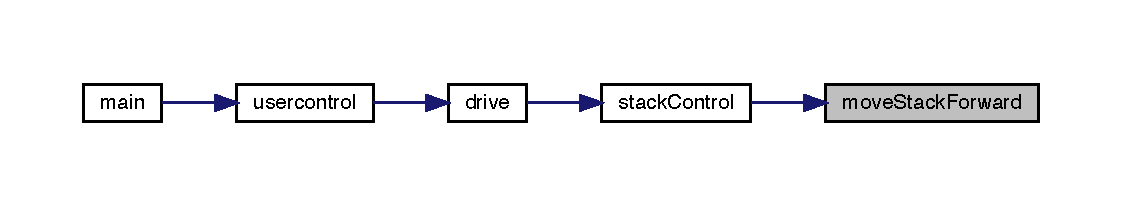
\includegraphics[width=350pt]{de/de5/drive_8cpp_a08a55986dab46203f1eeef50123cf4bd_a08a55986dab46203f1eeef50123cf4bd_icgraph}
\end{center}
\end{figure}
\mbox{\Hypertarget{drive_8cpp_ac522da2148fe1cfd9bea8c026e64ee7b_ac522da2148fe1cfd9bea8c026e64ee7b}\label{drive_8cpp_ac522da2148fe1cfd9bea8c026e64ee7b_ac522da2148fe1cfd9bea8c026e64ee7b}} 
\index{drive.cpp@{drive.cpp}!setSideSpeed@{setSideSpeed}}
\index{setSideSpeed@{setSideSpeed}!drive.cpp@{drive.cpp}}
\doxysubsubsection{\texorpdfstring{setSideSpeed()}{setSideSpeed()}}
{\footnotesize\ttfamily void set\+Side\+Speed (\begin{DoxyParamCaption}\item[{\mbox{\hyperlink{drive_8h_a2771dd4b083c12b0f13d534e3d1914dc_a2771dd4b083c12b0f13d534e3d1914dc}{Drive\+Side}}}]{side,  }\item[{int}]{speed }\end{DoxyParamCaption})}

Sets the speed of the designated drive side 
\begin{DoxyParams}{Parameters}
{\em side} & The Drive\+Side that is going to be powered \\
\hline
{\em speed} & The speed that the robot will move at between -\/100 -\/ 100 \\
\hline
\end{DoxyParams}
\begin{DoxyAuthor}{Author}
Michael Baraty 
\end{DoxyAuthor}
\begin{DoxyDate}{Date}
11/9/2019 
\end{DoxyDate}


Definition at line \mbox{\hyperlink{drive_8cpp_source_l00021}{21}} of file \mbox{\hyperlink{drive_8cpp_source}{drive.\+cpp}}.


\begin{DoxyCode}{0}
\DoxyCodeLine{00021                                              \{}
\DoxyCodeLine{00022   \textcolor{keywordflow}{if}(side == \mbox{\hyperlink{drive_8h_a2771dd4b083c12b0f13d534e3d1914dc_a2771dd4b083c12b0f13d534e3d1914dca684d325a7303f52e64011467ff5c5758}{DriveSide::LEFT}}) \{}
\DoxyCodeLine{00023     \mbox{\hyperlink{declarations_8h_ab24214b642128d0f3cb67e9b12e7d4fb_ab24214b642128d0f3cb67e9b12e7d4fb}{MOTOR\_BACK\_LEFT}}.spin(directionType::fwd, speed, velocityUnits::pct);}
\DoxyCodeLine{00024     \mbox{\hyperlink{declarations_8h_a8c6f6315caf1d81bf4d4d113d0f7bffc_a8c6f6315caf1d81bf4d4d113d0f7bffc}{MOTOR\_FRONT\_LEFT}}.spin(directionType::fwd, speed, velocityUnits::pct);}
\DoxyCodeLine{00025   \} \textcolor{keywordflow}{else} \textcolor{keywordflow}{if} (side == \mbox{\hyperlink{drive_8h_a2771dd4b083c12b0f13d534e3d1914dc_a2771dd4b083c12b0f13d534e3d1914dca21507b40c80068eda19865706fdc2403}{DriveSide::RIGHT}}) \{}
\DoxyCodeLine{00026     \mbox{\hyperlink{declarations_8h_adece81dedf91c2893ba42dc05135a575_adece81dedf91c2893ba42dc05135a575}{MOTOR\_BACK\_RIGHT}}.spin(directionType::fwd, speed, velocityUnits::pct);}
\DoxyCodeLine{00027     \mbox{\hyperlink{declarations_8h_ad6a9ea3d338421c5d709c32ae1aa42d8_ad6a9ea3d338421c5d709c32ae1aa42d8}{MOTOR\_FRONT\_RIGHT}}.spin(directionType::fwd, speed, velocityUnits::pct);}
\DoxyCodeLine{00028   \}}
\DoxyCodeLine{00029   \textcolor{keywordflow}{else} \{}
\DoxyCodeLine{00030     \mbox{\hyperlink{declarations_8h_a8c6f6315caf1d81bf4d4d113d0f7bffc_a8c6f6315caf1d81bf4d4d113d0f7bffc}{MOTOR\_FRONT\_LEFT}}.spin(directionType::fwd, speed, velocityUnits::pct);}
\DoxyCodeLine{00031     \mbox{\hyperlink{declarations_8h_ad6a9ea3d338421c5d709c32ae1aa42d8_ad6a9ea3d338421c5d709c32ae1aa42d8}{MOTOR\_FRONT\_RIGHT}}.spin(directionType::fwd, speed, velocityUnits::pct);}
\DoxyCodeLine{00032     \mbox{\hyperlink{declarations_8h_adece81dedf91c2893ba42dc05135a575_adece81dedf91c2893ba42dc05135a575}{MOTOR\_BACK\_RIGHT}}.spin(directionType::fwd, speed, velocityUnits::pct);}
\DoxyCodeLine{00033     \mbox{\hyperlink{declarations_8h_ab24214b642128d0f3cb67e9b12e7d4fb_ab24214b642128d0f3cb67e9b12e7d4fb}{MOTOR\_BACK\_LEFT}}.spin(directionType::fwd, speed, velocityUnits::pct);}
\DoxyCodeLine{00034   \}}
\DoxyCodeLine{00035 \}}

\end{DoxyCode}
Here is the caller graph for this function\+:\nopagebreak
\begin{figure}[H]
\begin{center}
\leavevmode
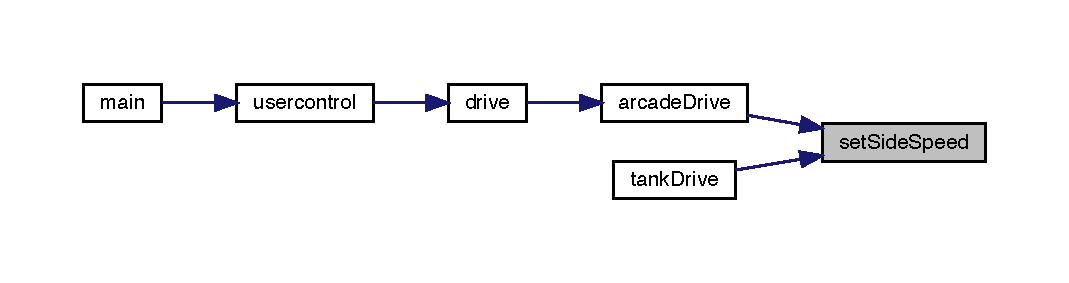
\includegraphics[width=350pt]{de/de5/drive_8cpp_ac522da2148fe1cfd9bea8c026e64ee7b_ac522da2148fe1cfd9bea8c026e64ee7b_icgraph}
\end{center}
\end{figure}
\mbox{\Hypertarget{drive_8cpp_abc3819041cf96aad1093752a3a5de31c_abc3819041cf96aad1093752a3a5de31c}\label{drive_8cpp_abc3819041cf96aad1093752a3a5de31c_abc3819041cf96aad1093752a3a5de31c}} 
\index{drive.cpp@{drive.cpp}!stackControl@{stackControl}}
\index{stackControl@{stackControl}!drive.cpp@{drive.cpp}}
\doxysubsubsection{\texorpdfstring{stackControl()}{stackControl()}}
{\footnotesize\ttfamily void stack\+Control (\begin{DoxyParamCaption}{ }\end{DoxyParamCaption})}

Reads the controller\textquotesingle{}s button inputs to initiate the stack mechanism\textquotesingle{}s movement while the button is being pressed \begin{DoxyAuthor}{Author}
Michael Baraty 
\end{DoxyAuthor}
\begin{DoxyDate}{Date}
11/9/2019 
\end{DoxyDate}


Definition at line \mbox{\hyperlink{drive_8cpp_source_l00077}{77}} of file \mbox{\hyperlink{drive_8cpp_source}{drive.\+cpp}}.


\begin{DoxyCode}{0}
\DoxyCodeLine{00077                     \{}
\DoxyCodeLine{00078   \textcolor{keywordflow}{if}(\mbox{\hyperlink{controller_8h_aff3b02388de758f0fe6d98930ea57626_aff3b02388de758f0fe6d98930ea57626}{buttonIsPressed}}(\mbox{\hyperlink{declarations_8h_ab04f8ff803f7f02c23e713402e13bf32_ab04f8ff803f7f02c23e713402e13bf32}{MASTER}}.ButtonX)) }
\DoxyCodeLine{00079     \mbox{\hyperlink{drive_8cpp_a08a55986dab46203f1eeef50123cf4bd_a08a55986dab46203f1eeef50123cf4bd}{moveStackForward}}();}
\DoxyCodeLine{00080   \textcolor{keywordflow}{else} \textcolor{keywordflow}{if}(\mbox{\hyperlink{controller_8h_aff3b02388de758f0fe6d98930ea57626_aff3b02388de758f0fe6d98930ea57626}{buttonIsPressed}}(\mbox{\hyperlink{declarations_8h_ab04f8ff803f7f02c23e713402e13bf32_ab04f8ff803f7f02c23e713402e13bf32}{MASTER}}.ButtonA))}
\DoxyCodeLine{00081     \mbox{\hyperlink{drive_8cpp_ac153148440cec552a2824c91569e1e5a_ac153148440cec552a2824c91569e1e5a}{moveStackBack}}();}
\DoxyCodeLine{00082   \textcolor{keywordflow}{else}\{}
\DoxyCodeLine{00083     \mbox{\hyperlink{declarations_8h_a212c888d64ffcd7e7b44a548fa0408a9_a212c888d64ffcd7e7b44a548fa0408a9}{MOTOR\_STACK}}.stop(brakeType::brake);}
\DoxyCodeLine{00084   \}}
\DoxyCodeLine{00085 \}}

\end{DoxyCode}
Here is the call graph for this function\+:\nopagebreak
\begin{figure}[H]
\begin{center}
\leavevmode
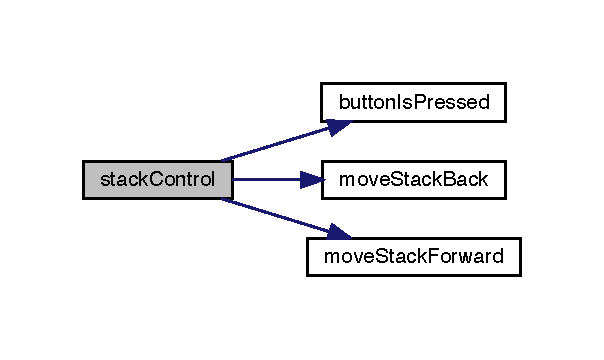
\includegraphics[width=290pt]{de/de5/drive_8cpp_abc3819041cf96aad1093752a3a5de31c_abc3819041cf96aad1093752a3a5de31c_cgraph}
\end{center}
\end{figure}
Here is the caller graph for this function\+:\nopagebreak
\begin{figure}[H]
\begin{center}
\leavevmode
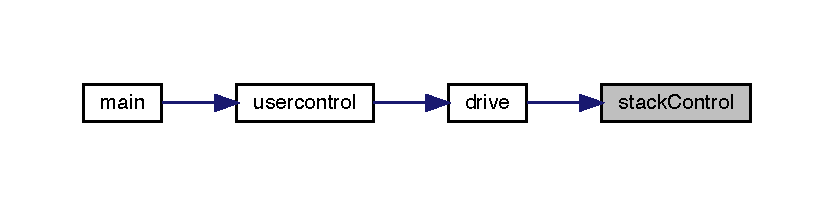
\includegraphics[width=350pt]{de/de5/drive_8cpp_abc3819041cf96aad1093752a3a5de31c_abc3819041cf96aad1093752a3a5de31c_icgraph}
\end{center}
\end{figure}
\mbox{\Hypertarget{drive_8cpp_ab8605578ac6dddeb3e511513523e3354_ab8605578ac6dddeb3e511513523e3354}\label{drive_8cpp_ab8605578ac6dddeb3e511513523e3354_ab8605578ac6dddeb3e511513523e3354}} 
\index{drive.cpp@{drive.cpp}!tankDrive@{tankDrive}}
\index{tankDrive@{tankDrive}!drive.cpp@{drive.cpp}}
\doxysubsubsection{\texorpdfstring{tankDrive()}{tankDrive()}}
{\footnotesize\ttfamily void tank\+Drive (\begin{DoxyParamCaption}{ }\end{DoxyParamCaption})}

Initiates the tank drive control configuration for the controller, with the left y axis for the left side and the right y axis for the right side \begin{DoxyAuthor}{Author}
Michael Baraty 
\end{DoxyAuthor}
\begin{DoxyDate}{Date}
11/9/2019 
\end{DoxyDate}


Definition at line \mbox{\hyperlink{drive_8cpp_source_l00052}{52}} of file \mbox{\hyperlink{drive_8cpp_source}{drive.\+cpp}}.


\begin{DoxyCode}{0}
\DoxyCodeLine{00052                  \{}
\DoxyCodeLine{00053   \textcolor{keywordtype}{int} l = \mbox{\hyperlink{declarations_8h_afb49f22bdd1e93218d02bb25e513e8a0_afb49f22bdd1e93218d02bb25e513e8a0}{SPEED\_MULTIPLIER}} * (.7  * (pow(\mbox{\hyperlink{controller_8h_a73be3a8649e7d561a68cd816420efbd9_a73be3a8649e7d561a68cd816420efbd9}{axisValue}}(\mbox{\hyperlink{declarations_8h_ab04f8ff803f7f02c23e713402e13bf32_ab04f8ff803f7f02c23e713402e13bf32}{MASTER}}.Axis3) / 9, 3) / 10));}
\DoxyCodeLine{00054   \textcolor{keywordtype}{int} r = \mbox{\hyperlink{declarations_8h_afb49f22bdd1e93218d02bb25e513e8a0_afb49f22bdd1e93218d02bb25e513e8a0}{SPEED\_MULTIPLIER}} * (.7  * (pow(\mbox{\hyperlink{controller_8h_a73be3a8649e7d561a68cd816420efbd9_a73be3a8649e7d561a68cd816420efbd9}{axisValue}}(\mbox{\hyperlink{declarations_8h_ab04f8ff803f7f02c23e713402e13bf32_ab04f8ff803f7f02c23e713402e13bf32}{MASTER}}.Axis2) / 9, 3) / 10));}
\DoxyCodeLine{00055   \textcolor{keywordtype}{int} speedLeft = abs(l) > \mbox{\hyperlink{declarations_8h_adceb947873623dd2a87f7f69e81fbd38_adceb947873623dd2a87f7f69e81fbd38}{THRESHOLD}}? l: 0;}
\DoxyCodeLine{00056   \textcolor{keywordtype}{int} speedRight = abs(r) > \mbox{\hyperlink{declarations_8h_adceb947873623dd2a87f7f69e81fbd38_adceb947873623dd2a87f7f69e81fbd38}{THRESHOLD}}? r: 0;}
\DoxyCodeLine{00057   }
\DoxyCodeLine{00058   \textcolor{keywordflow}{if}(\mbox{\hyperlink{drive_8cpp_ac84adc1c8ccd21c3c630031ad1ce5956_ac84adc1c8ccd21c3c630031ad1ce5956}{slowMode}})\{}
\DoxyCodeLine{00059     \mbox{\hyperlink{drive_8cpp_ac522da2148fe1cfd9bea8c026e64ee7b_ac522da2148fe1cfd9bea8c026e64ee7b}{setSideSpeed}}(\mbox{\hyperlink{drive_8h_a2771dd4b083c12b0f13d534e3d1914dc_a2771dd4b083c12b0f13d534e3d1914dca684d325a7303f52e64011467ff5c5758}{DriveSide::LEFT}}, speedLeft / 3);}
\DoxyCodeLine{00060      \mbox{\hyperlink{drive_8cpp_ac522da2148fe1cfd9bea8c026e64ee7b_ac522da2148fe1cfd9bea8c026e64ee7b}{setSideSpeed}}(\mbox{\hyperlink{drive_8h_a2771dd4b083c12b0f13d534e3d1914dc_a2771dd4b083c12b0f13d534e3d1914dca21507b40c80068eda19865706fdc2403}{DriveSide::RIGHT}}, speedRight / 3);}
\DoxyCodeLine{00061   \} \textcolor{keywordflow}{else} \{}
\DoxyCodeLine{00062     \mbox{\hyperlink{drive_8cpp_ac522da2148fe1cfd9bea8c026e64ee7b_ac522da2148fe1cfd9bea8c026e64ee7b}{setSideSpeed}}(\mbox{\hyperlink{drive_8h_a2771dd4b083c12b0f13d534e3d1914dc_a2771dd4b083c12b0f13d534e3d1914dca684d325a7303f52e64011467ff5c5758}{DriveSide::LEFT}}, speedLeft);}
\DoxyCodeLine{00063     \mbox{\hyperlink{drive_8cpp_ac522da2148fe1cfd9bea8c026e64ee7b_ac522da2148fe1cfd9bea8c026e64ee7b}{setSideSpeed}}(\mbox{\hyperlink{drive_8h_a2771dd4b083c12b0f13d534e3d1914dc_a2771dd4b083c12b0f13d534e3d1914dca21507b40c80068eda19865706fdc2403}{DriveSide::RIGHT}}, speedRight);}
\DoxyCodeLine{00064   \}}
\DoxyCodeLine{00065 \}}

\end{DoxyCode}
Here is the call graph for this function\+:\nopagebreak
\begin{figure}[H]
\begin{center}
\leavevmode
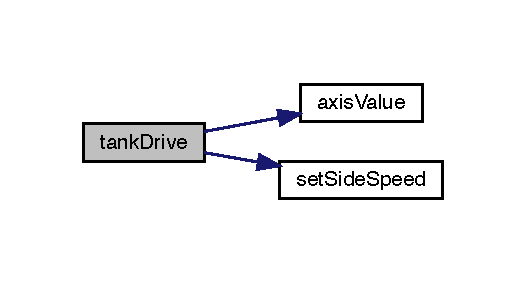
\includegraphics[width=253pt]{de/de5/drive_8cpp_ab8605578ac6dddeb3e511513523e3354_ab8605578ac6dddeb3e511513523e3354_cgraph}
\end{center}
\end{figure}


\doxysubsection{Variable Documentation}
\mbox{\Hypertarget{drive_8cpp_ac84adc1c8ccd21c3c630031ad1ce5956_ac84adc1c8ccd21c3c630031ad1ce5956}\label{drive_8cpp_ac84adc1c8ccd21c3c630031ad1ce5956_ac84adc1c8ccd21c3c630031ad1ce5956}} 
\index{drive.cpp@{drive.cpp}!slowMode@{slowMode}}
\index{slowMode@{slowMode}!drive.cpp@{drive.cpp}}
\doxysubsubsection{\texorpdfstring{slowMode}{slowMode}}
{\footnotesize\ttfamily bool slow\+Mode = false}



Definition at line \mbox{\hyperlink{drive_8cpp_source_l00005}{5}} of file \mbox{\hyperlink{drive_8cpp_source}{drive.\+cpp}}.


\hypertarget{drive_8cpp_source}{}\doxysection{drive.\+cpp}
\label{drive_8cpp_source}\index{src/drive.cpp@{src/drive.cpp}}

\begin{DoxyCode}{0}
\DoxyCodeLine{00001 \textcolor{preprocessor}{\#include "\mbox{\hyperlink{drive_8h}{drive.h}}"}}
\DoxyCodeLine{00002 \textcolor{preprocessor}{\#include "\mbox{\hyperlink{declarations_8h}{declarations.h}}"}}
\DoxyCodeLine{00003 \textcolor{preprocessor}{\#include "\mbox{\hyperlink{auton_8h}{auton.h}}"}}
\DoxyCodeLine{00004 }
\DoxyCodeLine{\Hypertarget{drive_8cpp_source_l00005}\mbox{\hyperlink{drive_8cpp_ac84adc1c8ccd21c3c630031ad1ce5956_ac84adc1c8ccd21c3c630031ad1ce5956}{00005}} \textcolor{keywordtype}{bool} \mbox{\hyperlink{drive_8cpp_ac84adc1c8ccd21c3c630031ad1ce5956_ac84adc1c8ccd21c3c630031ad1ce5956}{slowMode}} = \textcolor{keyword}{false};}
\DoxyCodeLine{00006 }
\DoxyCodeLine{\Hypertarget{drive_8cpp_source_l00007}\mbox{\hyperlink{drive_8cpp_a928e32686c7e00c1ecde24c3da3019f7_a928e32686c7e00c1ecde24c3da3019f7}{00007}} \textcolor{keywordtype}{void} \mbox{\hyperlink{drive_8cpp_a928e32686c7e00c1ecde24c3da3019f7_a928e32686c7e00c1ecde24c3da3019f7}{drive}}() \{}
\DoxyCodeLine{00008   \mbox{\hyperlink{drive_8cpp_a6ff8820b82f28a73c88a746ddacb26bb_a6ff8820b82f28a73c88a746ddacb26bb}{arcadeDrive}}();}
\DoxyCodeLine{00009   \mbox{\hyperlink{drive_8cpp_abc3819041cf96aad1093752a3a5de31c_abc3819041cf96aad1093752a3a5de31c}{stackControl}}();}
\DoxyCodeLine{00010   \mbox{\hyperlink{drive_8cpp_adde1067b42b4de65ff20afb8901f7643_adde1067b42b4de65ff20afb8901f7643}{armControl}}();}
\DoxyCodeLine{00011   \mbox{\hyperlink{drive_8cpp_a8afb2a071b21d98c49d5888a7b380ba6_a8afb2a071b21d98c49d5888a7b380ba6}{intakeControl}}();}
\DoxyCodeLine{00012 }
\DoxyCodeLine{00013   \textcolor{keywordflow}{if}(\mbox{\hyperlink{controller_8h_aff3b02388de758f0fe6d98930ea57626_aff3b02388de758f0fe6d98930ea57626}{buttonIsPressed}}(\mbox{\hyperlink{declarations_8h_ab04f8ff803f7f02c23e713402e13bf32_ab04f8ff803f7f02c23e713402e13bf32}{MASTER}}.ButtonUp))\{}
\DoxyCodeLine{00014     \mbox{\hyperlink{drive_8cpp_ac84adc1c8ccd21c3c630031ad1ce5956_ac84adc1c8ccd21c3c630031ad1ce5956}{slowMode}} = \textcolor{keyword}{false};}
\DoxyCodeLine{00015   \} \textcolor{keywordflow}{else} \textcolor{keywordflow}{if}(\mbox{\hyperlink{controller_8h_aff3b02388de758f0fe6d98930ea57626_aff3b02388de758f0fe6d98930ea57626}{buttonIsPressed}}(\mbox{\hyperlink{declarations_8h_ab04f8ff803f7f02c23e713402e13bf32_ab04f8ff803f7f02c23e713402e13bf32}{MASTER}}.ButtonDown))\{}
\DoxyCodeLine{00016     \mbox{\hyperlink{drive_8cpp_ac84adc1c8ccd21c3c630031ad1ce5956_ac84adc1c8ccd21c3c630031ad1ce5956}{slowMode}} = \textcolor{keyword}{true};}
\DoxyCodeLine{00017   \}}
\DoxyCodeLine{00018 }
\DoxyCodeLine{00019 \}}
\DoxyCodeLine{00020 }
\DoxyCodeLine{\Hypertarget{drive_8cpp_source_l00021}\mbox{\hyperlink{drive_8cpp_ac522da2148fe1cfd9bea8c026e64ee7b_ac522da2148fe1cfd9bea8c026e64ee7b}{00021}} \textcolor{keywordtype}{void} \mbox{\hyperlink{drive_8cpp_ac522da2148fe1cfd9bea8c026e64ee7b_ac522da2148fe1cfd9bea8c026e64ee7b}{setSideSpeed}}(\mbox{\hyperlink{drive_8h_a2771dd4b083c12b0f13d534e3d1914dc_a2771dd4b083c12b0f13d534e3d1914dc}{DriveSide}} side, \textcolor{keywordtype}{int} speed) \{}
\DoxyCodeLine{00022   \textcolor{keywordflow}{if}(side == \mbox{\hyperlink{drive_8h_a2771dd4b083c12b0f13d534e3d1914dc_a2771dd4b083c12b0f13d534e3d1914dca684d325a7303f52e64011467ff5c5758}{DriveSide::LEFT}}) \{}
\DoxyCodeLine{00023     \mbox{\hyperlink{declarations_8h_ab24214b642128d0f3cb67e9b12e7d4fb_ab24214b642128d0f3cb67e9b12e7d4fb}{MOTOR\_BACK\_LEFT}}.spin(directionType::fwd, speed, velocityUnits::pct);}
\DoxyCodeLine{00024     \mbox{\hyperlink{declarations_8h_a8c6f6315caf1d81bf4d4d113d0f7bffc_a8c6f6315caf1d81bf4d4d113d0f7bffc}{MOTOR\_FRONT\_LEFT}}.spin(directionType::fwd, speed, velocityUnits::pct);}
\DoxyCodeLine{00025   \} \textcolor{keywordflow}{else} \textcolor{keywordflow}{if} (side == \mbox{\hyperlink{drive_8h_a2771dd4b083c12b0f13d534e3d1914dc_a2771dd4b083c12b0f13d534e3d1914dca21507b40c80068eda19865706fdc2403}{DriveSide::RIGHT}}) \{}
\DoxyCodeLine{00026     \mbox{\hyperlink{declarations_8h_adece81dedf91c2893ba42dc05135a575_adece81dedf91c2893ba42dc05135a575}{MOTOR\_BACK\_RIGHT}}.spin(directionType::fwd, speed, velocityUnits::pct);}
\DoxyCodeLine{00027     \mbox{\hyperlink{declarations_8h_ad6a9ea3d338421c5d709c32ae1aa42d8_ad6a9ea3d338421c5d709c32ae1aa42d8}{MOTOR\_FRONT\_RIGHT}}.spin(directionType::fwd, speed, velocityUnits::pct);}
\DoxyCodeLine{00028   \}}
\DoxyCodeLine{00029   \textcolor{keywordflow}{else} \{}
\DoxyCodeLine{00030     \mbox{\hyperlink{declarations_8h_a8c6f6315caf1d81bf4d4d113d0f7bffc_a8c6f6315caf1d81bf4d4d113d0f7bffc}{MOTOR\_FRONT\_LEFT}}.spin(directionType::fwd, speed, velocityUnits::pct);}
\DoxyCodeLine{00031     \mbox{\hyperlink{declarations_8h_ad6a9ea3d338421c5d709c32ae1aa42d8_ad6a9ea3d338421c5d709c32ae1aa42d8}{MOTOR\_FRONT\_RIGHT}}.spin(directionType::fwd, speed, velocityUnits::pct);}
\DoxyCodeLine{00032     \mbox{\hyperlink{declarations_8h_adece81dedf91c2893ba42dc05135a575_adece81dedf91c2893ba42dc05135a575}{MOTOR\_BACK\_RIGHT}}.spin(directionType::fwd, speed, velocityUnits::pct);}
\DoxyCodeLine{00033     \mbox{\hyperlink{declarations_8h_ab24214b642128d0f3cb67e9b12e7d4fb_ab24214b642128d0f3cb67e9b12e7d4fb}{MOTOR\_BACK\_LEFT}}.spin(directionType::fwd, speed, velocityUnits::pct);}
\DoxyCodeLine{00034   \}}
\DoxyCodeLine{00035 \}}
\DoxyCodeLine{00036 }
\DoxyCodeLine{\Hypertarget{drive_8cpp_source_l00037}\mbox{\hyperlink{drive_8cpp_a6ff8820b82f28a73c88a746ddacb26bb_a6ff8820b82f28a73c88a746ddacb26bb}{00037}} \textcolor{keywordtype}{void} \mbox{\hyperlink{drive_8cpp_a6ff8820b82f28a73c88a746ddacb26bb_a6ff8820b82f28a73c88a746ddacb26bb}{arcadeDrive}}() \{}
\DoxyCodeLine{00038   \textcolor{keywordtype}{int} x = \mbox{\hyperlink{declarations_8h_afb49f22bdd1e93218d02bb25e513e8a0_afb49f22bdd1e93218d02bb25e513e8a0}{SPEED\_MULTIPLIER}}  * -\/\mbox{\hyperlink{controller_8h_a73be3a8649e7d561a68cd816420efbd9_a73be3a8649e7d561a68cd816420efbd9}{axisValue}}(\mbox{\hyperlink{declarations_8h_ab04f8ff803f7f02c23e713402e13bf32_ab04f8ff803f7f02c23e713402e13bf32}{MASTER}}.Axis1);}
\DoxyCodeLine{00039   \textcolor{keywordtype}{int} y = \mbox{\hyperlink{declarations_8h_afb49f22bdd1e93218d02bb25e513e8a0_afb49f22bdd1e93218d02bb25e513e8a0}{SPEED\_MULTIPLIER}} * (.7  * (pow(-\/\mbox{\hyperlink{controller_8h_a73be3a8649e7d561a68cd816420efbd9_a73be3a8649e7d561a68cd816420efbd9}{axisValue}}(\mbox{\hyperlink{declarations_8h_ab04f8ff803f7f02c23e713402e13bf32_ab04f8ff803f7f02c23e713402e13bf32}{MASTER}}.Axis3) / 9, 3) / 10));}
\DoxyCodeLine{00040   \textcolor{keywordtype}{int} speedLeft = abs(x + y) > \mbox{\hyperlink{declarations_8h_adceb947873623dd2a87f7f69e81fbd38_adceb947873623dd2a87f7f69e81fbd38}{THRESHOLD}}? -\/(x + y): 0;}
\DoxyCodeLine{00041   \textcolor{keywordtype}{int} speedRight = abs(x -\/ y) > \mbox{\hyperlink{declarations_8h_adceb947873623dd2a87f7f69e81fbd38_adceb947873623dd2a87f7f69e81fbd38}{THRESHOLD}}? (x -\/ y): 0;}
\DoxyCodeLine{00042 }
\DoxyCodeLine{00043   \textcolor{keywordflow}{if}(\mbox{\hyperlink{drive_8cpp_ac84adc1c8ccd21c3c630031ad1ce5956_ac84adc1c8ccd21c3c630031ad1ce5956}{slowMode}})\{}
\DoxyCodeLine{00044     \mbox{\hyperlink{drive_8cpp_ac522da2148fe1cfd9bea8c026e64ee7b_ac522da2148fe1cfd9bea8c026e64ee7b}{setSideSpeed}}(\mbox{\hyperlink{drive_8h_a2771dd4b083c12b0f13d534e3d1914dc_a2771dd4b083c12b0f13d534e3d1914dca684d325a7303f52e64011467ff5c5758}{DriveSide::LEFT}}, speedLeft / 3);}
\DoxyCodeLine{00045      \mbox{\hyperlink{drive_8cpp_ac522da2148fe1cfd9bea8c026e64ee7b_ac522da2148fe1cfd9bea8c026e64ee7b}{setSideSpeed}}(\mbox{\hyperlink{drive_8h_a2771dd4b083c12b0f13d534e3d1914dc_a2771dd4b083c12b0f13d534e3d1914dca21507b40c80068eda19865706fdc2403}{DriveSide::RIGHT}}, speedRight / 3);}
\DoxyCodeLine{00046   \} \textcolor{keywordflow}{else} \{}
\DoxyCodeLine{00047     \mbox{\hyperlink{drive_8cpp_ac522da2148fe1cfd9bea8c026e64ee7b_ac522da2148fe1cfd9bea8c026e64ee7b}{setSideSpeed}}(\mbox{\hyperlink{drive_8h_a2771dd4b083c12b0f13d534e3d1914dc_a2771dd4b083c12b0f13d534e3d1914dca684d325a7303f52e64011467ff5c5758}{DriveSide::LEFT}}, speedLeft);}
\DoxyCodeLine{00048     \mbox{\hyperlink{drive_8cpp_ac522da2148fe1cfd9bea8c026e64ee7b_ac522da2148fe1cfd9bea8c026e64ee7b}{setSideSpeed}}(\mbox{\hyperlink{drive_8h_a2771dd4b083c12b0f13d534e3d1914dc_a2771dd4b083c12b0f13d534e3d1914dca21507b40c80068eda19865706fdc2403}{DriveSide::RIGHT}}, speedRight);}
\DoxyCodeLine{00049   \}}
\DoxyCodeLine{00050 \}}
\DoxyCodeLine{00051 }
\DoxyCodeLine{\Hypertarget{drive_8cpp_source_l00052}\mbox{\hyperlink{drive_8cpp_ab8605578ac6dddeb3e511513523e3354_ab8605578ac6dddeb3e511513523e3354}{00052}} \textcolor{keywordtype}{void} \mbox{\hyperlink{drive_8cpp_ab8605578ac6dddeb3e511513523e3354_ab8605578ac6dddeb3e511513523e3354}{tankDrive}}() \{}
\DoxyCodeLine{00053   \textcolor{keywordtype}{int} l = \mbox{\hyperlink{declarations_8h_afb49f22bdd1e93218d02bb25e513e8a0_afb49f22bdd1e93218d02bb25e513e8a0}{SPEED\_MULTIPLIER}} * (.7  * (pow(\mbox{\hyperlink{controller_8h_a73be3a8649e7d561a68cd816420efbd9_a73be3a8649e7d561a68cd816420efbd9}{axisValue}}(\mbox{\hyperlink{declarations_8h_ab04f8ff803f7f02c23e713402e13bf32_ab04f8ff803f7f02c23e713402e13bf32}{MASTER}}.Axis3) / 9, 3) / 10));}
\DoxyCodeLine{00054   \textcolor{keywordtype}{int} r = \mbox{\hyperlink{declarations_8h_afb49f22bdd1e93218d02bb25e513e8a0_afb49f22bdd1e93218d02bb25e513e8a0}{SPEED\_MULTIPLIER}} * (.7  * (pow(\mbox{\hyperlink{controller_8h_a73be3a8649e7d561a68cd816420efbd9_a73be3a8649e7d561a68cd816420efbd9}{axisValue}}(\mbox{\hyperlink{declarations_8h_ab04f8ff803f7f02c23e713402e13bf32_ab04f8ff803f7f02c23e713402e13bf32}{MASTER}}.Axis2) / 9, 3) / 10));}
\DoxyCodeLine{00055   \textcolor{keywordtype}{int} speedLeft = abs(l) > \mbox{\hyperlink{declarations_8h_adceb947873623dd2a87f7f69e81fbd38_adceb947873623dd2a87f7f69e81fbd38}{THRESHOLD}}? l: 0;}
\DoxyCodeLine{00056   \textcolor{keywordtype}{int} speedRight = abs(r) > \mbox{\hyperlink{declarations_8h_adceb947873623dd2a87f7f69e81fbd38_adceb947873623dd2a87f7f69e81fbd38}{THRESHOLD}}? r: 0;}
\DoxyCodeLine{00057   }
\DoxyCodeLine{00058   \textcolor{keywordflow}{if}(\mbox{\hyperlink{drive_8cpp_ac84adc1c8ccd21c3c630031ad1ce5956_ac84adc1c8ccd21c3c630031ad1ce5956}{slowMode}})\{}
\DoxyCodeLine{00059     \mbox{\hyperlink{drive_8cpp_ac522da2148fe1cfd9bea8c026e64ee7b_ac522da2148fe1cfd9bea8c026e64ee7b}{setSideSpeed}}(\mbox{\hyperlink{drive_8h_a2771dd4b083c12b0f13d534e3d1914dc_a2771dd4b083c12b0f13d534e3d1914dca684d325a7303f52e64011467ff5c5758}{DriveSide::LEFT}}, speedLeft / 3);}
\DoxyCodeLine{00060      \mbox{\hyperlink{drive_8cpp_ac522da2148fe1cfd9bea8c026e64ee7b_ac522da2148fe1cfd9bea8c026e64ee7b}{setSideSpeed}}(\mbox{\hyperlink{drive_8h_a2771dd4b083c12b0f13d534e3d1914dc_a2771dd4b083c12b0f13d534e3d1914dca21507b40c80068eda19865706fdc2403}{DriveSide::RIGHT}}, speedRight / 3);}
\DoxyCodeLine{00061   \} \textcolor{keywordflow}{else} \{}
\DoxyCodeLine{00062     \mbox{\hyperlink{drive_8cpp_ac522da2148fe1cfd9bea8c026e64ee7b_ac522da2148fe1cfd9bea8c026e64ee7b}{setSideSpeed}}(\mbox{\hyperlink{drive_8h_a2771dd4b083c12b0f13d534e3d1914dc_a2771dd4b083c12b0f13d534e3d1914dca684d325a7303f52e64011467ff5c5758}{DriveSide::LEFT}}, speedLeft);}
\DoxyCodeLine{00063     \mbox{\hyperlink{drive_8cpp_ac522da2148fe1cfd9bea8c026e64ee7b_ac522da2148fe1cfd9bea8c026e64ee7b}{setSideSpeed}}(\mbox{\hyperlink{drive_8h_a2771dd4b083c12b0f13d534e3d1914dc_a2771dd4b083c12b0f13d534e3d1914dca21507b40c80068eda19865706fdc2403}{DriveSide::RIGHT}}, speedRight);}
\DoxyCodeLine{00064   \}}
\DoxyCodeLine{00065 \}}
\DoxyCodeLine{00066 }
\DoxyCodeLine{\Hypertarget{drive_8cpp_source_l00067}\mbox{\hyperlink{drive_8cpp_a08a55986dab46203f1eeef50123cf4bd_a08a55986dab46203f1eeef50123cf4bd}{00067}} \textcolor{keywordtype}{void} \mbox{\hyperlink{drive_8cpp_a08a55986dab46203f1eeef50123cf4bd_a08a55986dab46203f1eeef50123cf4bd}{moveStackForward}}() \{}
\DoxyCodeLine{00068   \textcolor{keywordtype}{double} \textcolor{keyword}{final} = 1.5; }
\DoxyCodeLine{00069   \mbox{\hyperlink{declarations_8h_a212c888d64ffcd7e7b44a548fa0408a9_a212c888d64ffcd7e7b44a548fa0408a9}{MOTOR\_STACK}}.startSpinTo(10, rotationUnits::rev, 30, velocityUnits::pct);}
\DoxyCodeLine{00070 \}}
\DoxyCodeLine{00071 }
\DoxyCodeLine{\Hypertarget{drive_8cpp_source_l00072}\mbox{\hyperlink{drive_8cpp_ac153148440cec552a2824c91569e1e5a_ac153148440cec552a2824c91569e1e5a}{00072}} \textcolor{keywordtype}{void} \mbox{\hyperlink{drive_8cpp_ac153148440cec552a2824c91569e1e5a_ac153148440cec552a2824c91569e1e5a}{moveStackBack}}() \{}
\DoxyCodeLine{00073   \textcolor{keywordtype}{double} \textcolor{keyword}{final} = 0;}
\DoxyCodeLine{00074   \mbox{\hyperlink{declarations_8h_a212c888d64ffcd7e7b44a548fa0408a9_a212c888d64ffcd7e7b44a548fa0408a9}{MOTOR\_STACK}}.startSpinTo(-\/10, rotationUnits::rev, 80, velocityUnits::pct); }
\DoxyCodeLine{00075 \}}
\DoxyCodeLine{00076 }
\DoxyCodeLine{\Hypertarget{drive_8cpp_source_l00077}\mbox{\hyperlink{drive_8cpp_abc3819041cf96aad1093752a3a5de31c_abc3819041cf96aad1093752a3a5de31c}{00077}} \textcolor{keywordtype}{void} \mbox{\hyperlink{drive_8cpp_abc3819041cf96aad1093752a3a5de31c_abc3819041cf96aad1093752a3a5de31c}{stackControl}}() \{}
\DoxyCodeLine{00078   \textcolor{keywordflow}{if}(\mbox{\hyperlink{controller_8h_aff3b02388de758f0fe6d98930ea57626_aff3b02388de758f0fe6d98930ea57626}{buttonIsPressed}}(\mbox{\hyperlink{declarations_8h_ab04f8ff803f7f02c23e713402e13bf32_ab04f8ff803f7f02c23e713402e13bf32}{MASTER}}.ButtonX)) }
\DoxyCodeLine{00079     \mbox{\hyperlink{drive_8cpp_a08a55986dab46203f1eeef50123cf4bd_a08a55986dab46203f1eeef50123cf4bd}{moveStackForward}}();}
\DoxyCodeLine{00080   \textcolor{keywordflow}{else} \textcolor{keywordflow}{if}(\mbox{\hyperlink{controller_8h_aff3b02388de758f0fe6d98930ea57626_aff3b02388de758f0fe6d98930ea57626}{buttonIsPressed}}(\mbox{\hyperlink{declarations_8h_ab04f8ff803f7f02c23e713402e13bf32_ab04f8ff803f7f02c23e713402e13bf32}{MASTER}}.ButtonA))}
\DoxyCodeLine{00081     \mbox{\hyperlink{drive_8cpp_ac153148440cec552a2824c91569e1e5a_ac153148440cec552a2824c91569e1e5a}{moveStackBack}}();}
\DoxyCodeLine{00082   \textcolor{keywordflow}{else}\{}
\DoxyCodeLine{00083     \mbox{\hyperlink{declarations_8h_a212c888d64ffcd7e7b44a548fa0408a9_a212c888d64ffcd7e7b44a548fa0408a9}{MOTOR\_STACK}}.stop(brakeType::brake);}
\DoxyCodeLine{00084   \}}
\DoxyCodeLine{00085 \}}
\DoxyCodeLine{00086 }
\DoxyCodeLine{\Hypertarget{drive_8cpp_source_l00087}\mbox{\hyperlink{drive_8cpp_adf7b0afb3a8dcf884db533b0217b0543_adf7b0afb3a8dcf884db533b0217b0543}{00087}} \textcolor{keywordtype}{void} \mbox{\hyperlink{drive_8cpp_adf7b0afb3a8dcf884db533b0217b0543_adf7b0afb3a8dcf884db533b0217b0543}{armUp}}()\{}
\DoxyCodeLine{00088   \mbox{\hyperlink{declarations_8h_a9a834f9a2c804ef0d65ed2f68c10a61a_a9a834f9a2c804ef0d65ed2f68c10a61a}{MOTOR\_ARM}}.startSpinTo(60.6, rotationUnits::rev, 100, velocityUnits::pct);}
\DoxyCodeLine{00089   \textcolor{comment}{//realValue 6.6}}
\DoxyCodeLine{00090 \}}
\DoxyCodeLine{00091 }
\DoxyCodeLine{\Hypertarget{drive_8cpp_source_l00092}\mbox{\hyperlink{drive_8cpp_ab1850cc7cdb69057fe29f45eefe7ec90_ab1850cc7cdb69057fe29f45eefe7ec90}{00092}} \textcolor{keywordtype}{void} \mbox{\hyperlink{drive_8cpp_ab1850cc7cdb69057fe29f45eefe7ec90_ab1850cc7cdb69057fe29f45eefe7ec90}{armDown}}()\{}
\DoxyCodeLine{00093   \mbox{\hyperlink{declarations_8h_a9a834f9a2c804ef0d65ed2f68c10a61a_a9a834f9a2c804ef0d65ed2f68c10a61a}{MOTOR\_ARM}}.startSpinTo(-\/10, rotationUnits::rev, 100, velocityUnits::pct);}
\DoxyCodeLine{00094   \textcolor{comment}{//realValue 0}}
\DoxyCodeLine{00095 \}}
\DoxyCodeLine{00096 }
\DoxyCodeLine{\Hypertarget{drive_8cpp_source_l00097}\mbox{\hyperlink{drive_8cpp_adde1067b42b4de65ff20afb8901f7643_adde1067b42b4de65ff20afb8901f7643}{00097}} \textcolor{keywordtype}{void} \mbox{\hyperlink{drive_8cpp_adde1067b42b4de65ff20afb8901f7643_adde1067b42b4de65ff20afb8901f7643}{armControl}}()\{}
\DoxyCodeLine{00098   \textcolor{keywordflow}{if}(\mbox{\hyperlink{controller_8h_aff3b02388de758f0fe6d98930ea57626_aff3b02388de758f0fe6d98930ea57626}{buttonIsPressed}}(\mbox{\hyperlink{declarations_8h_ab04f8ff803f7f02c23e713402e13bf32_ab04f8ff803f7f02c23e713402e13bf32}{MASTER}}.ButtonR1))\{}
\DoxyCodeLine{00099     \mbox{\hyperlink{drive_8cpp_adf7b0afb3a8dcf884db533b0217b0543_adf7b0afb3a8dcf884db533b0217b0543}{armUp}}();}
\DoxyCodeLine{00100   \}}
\DoxyCodeLine{00101   \textcolor{keywordflow}{else} \textcolor{keywordflow}{if} (\mbox{\hyperlink{controller_8h_aff3b02388de758f0fe6d98930ea57626_aff3b02388de758f0fe6d98930ea57626}{buttonIsPressed}}(\mbox{\hyperlink{declarations_8h_ab04f8ff803f7f02c23e713402e13bf32_ab04f8ff803f7f02c23e713402e13bf32}{MASTER}}.ButtonR2)) \{}
\DoxyCodeLine{00102     \mbox{\hyperlink{drive_8cpp_ab1850cc7cdb69057fe29f45eefe7ec90_ab1850cc7cdb69057fe29f45eefe7ec90}{armDown}}();}
\DoxyCodeLine{00103   \}}
\DoxyCodeLine{00104   \textcolor{keywordflow}{else} \{}
\DoxyCodeLine{00105     \mbox{\hyperlink{declarations_8h_a9a834f9a2c804ef0d65ed2f68c10a61a_a9a834f9a2c804ef0d65ed2f68c10a61a}{MOTOR\_ARM}}.stop(brakeType::hold);}
\DoxyCodeLine{00106   \}}
\DoxyCodeLine{00107 \}}
\DoxyCodeLine{00108 }
\DoxyCodeLine{\Hypertarget{drive_8cpp_source_l00109}\mbox{\hyperlink{drive_8cpp_aa0846c73538fc48569a7c7c3689a59f0_aa0846c73538fc48569a7c7c3689a59f0}{00109}} \textcolor{keywordtype}{void} \mbox{\hyperlink{drive_8cpp_aa0846c73538fc48569a7c7c3689a59f0_aa0846c73538fc48569a7c7c3689a59f0}{intakeIn}}() \{}
\DoxyCodeLine{00110   \textcolor{keywordflow}{if}(!\mbox{\hyperlink{drive_8cpp_ac84adc1c8ccd21c3c630031ad1ce5956_ac84adc1c8ccd21c3c630031ad1ce5956}{slowMode}}) \{}
\DoxyCodeLine{00111     \mbox{\hyperlink{declarations_8h_a34de211d15bfb3c0ac450597fd96b4fc_a34de211d15bfb3c0ac450597fd96b4fc}{MOTOR\_INTAKE\_A}}.spin(directionType::fwd, 100, velocityUnits::pct);}
\DoxyCodeLine{00112     \mbox{\hyperlink{declarations_8h_a5ae79e7ed71b0b94b3983c22c60c2eaa_a5ae79e7ed71b0b94b3983c22c60c2eaa}{MOTOR\_INTAKE\_B}}.spin(directionType::fwd, 100, velocityUnits::pct);}
\DoxyCodeLine{00113   \} \textcolor{keywordflow}{else} \{}
\DoxyCodeLine{00114     \mbox{\hyperlink{declarations_8h_a34de211d15bfb3c0ac450597fd96b4fc_a34de211d15bfb3c0ac450597fd96b4fc}{MOTOR\_INTAKE\_A}}.spin(directionType::fwd, (100), velocityUnits::pct);}
\DoxyCodeLine{00115     \mbox{\hyperlink{declarations_8h_a5ae79e7ed71b0b94b3983c22c60c2eaa_a5ae79e7ed71b0b94b3983c22c60c2eaa}{MOTOR\_INTAKE\_B}}.spin(directionType::fwd, (100), velocityUnits::pct);}
\DoxyCodeLine{00116   \}}
\DoxyCodeLine{00117 \}}
\DoxyCodeLine{00118 }
\DoxyCodeLine{\Hypertarget{drive_8cpp_source_l00119}\mbox{\hyperlink{drive_8cpp_aaca1ffa87592c1c5783fe6e18f9c655b_aaca1ffa87592c1c5783fe6e18f9c655b}{00119}} \textcolor{keywordtype}{void} \mbox{\hyperlink{drive_8cpp_aaca1ffa87592c1c5783fe6e18f9c655b_aaca1ffa87592c1c5783fe6e18f9c655b}{intakeOut}}() \{}
\DoxyCodeLine{00120    \textcolor{keywordflow}{if}(!\mbox{\hyperlink{drive_8cpp_ac84adc1c8ccd21c3c630031ad1ce5956_ac84adc1c8ccd21c3c630031ad1ce5956}{slowMode}}) \{}
\DoxyCodeLine{00121     \mbox{\hyperlink{declarations_8h_a34de211d15bfb3c0ac450597fd96b4fc_a34de211d15bfb3c0ac450597fd96b4fc}{MOTOR\_INTAKE\_A}}.spin(directionType::rev, 100, velocityUnits::pct);}
\DoxyCodeLine{00122     \mbox{\hyperlink{declarations_8h_a5ae79e7ed71b0b94b3983c22c60c2eaa_a5ae79e7ed71b0b94b3983c22c60c2eaa}{MOTOR\_INTAKE\_B}}.spin(directionType::rev, 100, velocityUnits::pct);}
\DoxyCodeLine{00123   \} \textcolor{keywordflow}{else} \{}
\DoxyCodeLine{00124     \mbox{\hyperlink{declarations_8h_a34de211d15bfb3c0ac450597fd96b4fc_a34de211d15bfb3c0ac450597fd96b4fc}{MOTOR\_INTAKE\_A}}.spin(directionType::rev, .5*(100), velocityUnits::pct);}
\DoxyCodeLine{00125     \mbox{\hyperlink{declarations_8h_a5ae79e7ed71b0b94b3983c22c60c2eaa_a5ae79e7ed71b0b94b3983c22c60c2eaa}{MOTOR\_INTAKE\_B}}.spin(directionType::rev, .5*(100), velocityUnits::pct);}
\DoxyCodeLine{00126   \}}
\DoxyCodeLine{00127 \}}
\DoxyCodeLine{00128 }
\DoxyCodeLine{\Hypertarget{drive_8cpp_source_l00129}\mbox{\hyperlink{drive_8cpp_a8afb2a071b21d98c49d5888a7b380ba6_a8afb2a071b21d98c49d5888a7b380ba6}{00129}} \textcolor{keywordtype}{void} \mbox{\hyperlink{drive_8cpp_a8afb2a071b21d98c49d5888a7b380ba6_a8afb2a071b21d98c49d5888a7b380ba6}{intakeControl}}() \{}
\DoxyCodeLine{00130   \textcolor{keywordflow}{if}(\mbox{\hyperlink{controller_8h_aff3b02388de758f0fe6d98930ea57626_aff3b02388de758f0fe6d98930ea57626}{buttonIsPressed}}(\mbox{\hyperlink{declarations_8h_ab04f8ff803f7f02c23e713402e13bf32_ab04f8ff803f7f02c23e713402e13bf32}{MASTER}}.ButtonL1))\{}
\DoxyCodeLine{00131     \mbox{\hyperlink{drive_8cpp_aa0846c73538fc48569a7c7c3689a59f0_aa0846c73538fc48569a7c7c3689a59f0}{intakeIn}}();}
\DoxyCodeLine{00132   \}}
\DoxyCodeLine{00133   \textcolor{keywordflow}{else} \textcolor{keywordflow}{if} (\mbox{\hyperlink{controller_8h_aff3b02388de758f0fe6d98930ea57626_aff3b02388de758f0fe6d98930ea57626}{buttonIsPressed}}(\mbox{\hyperlink{declarations_8h_ab04f8ff803f7f02c23e713402e13bf32_ab04f8ff803f7f02c23e713402e13bf32}{MASTER}}.ButtonL2)) \{}
\DoxyCodeLine{00134     \mbox{\hyperlink{drive_8cpp_aaca1ffa87592c1c5783fe6e18f9c655b_aaca1ffa87592c1c5783fe6e18f9c655b}{intakeOut}}();}
\DoxyCodeLine{00135   \}}
\DoxyCodeLine{00136   \textcolor{keywordflow}{else} \{}
\DoxyCodeLine{00137     \mbox{\hyperlink{declarations_8h_a34de211d15bfb3c0ac450597fd96b4fc_a34de211d15bfb3c0ac450597fd96b4fc}{MOTOR\_INTAKE\_A}}.stop(brakeType::hold);}
\DoxyCodeLine{00138     \mbox{\hyperlink{declarations_8h_a5ae79e7ed71b0b94b3983c22c60c2eaa_a5ae79e7ed71b0b94b3983c22c60c2eaa}{MOTOR\_INTAKE\_B}}.stop(brakeType::hold);}
\DoxyCodeLine{00139   \}}
\DoxyCodeLine{00140 \}}
\DoxyCodeLine{00141 }
\DoxyCodeLine{00142 }

\end{DoxyCode}

\hypertarget{init_8cpp}{}\subsection{src/init.cpp File Reference}
\label{init_8cpp}\index{src/init.\+cpp@{src/init.\+cpp}}
{\ttfamily \#include \char`\"{}init.\+h\char`\"{}}\newline

\hypertarget{init_8cpp_source}{}\doxysection{init.\+cpp}
\label{init_8cpp_source}\index{src/init.cpp@{src/init.cpp}}

\begin{DoxyCode}{0}
\DoxyCodeLine{00001 \textcolor{preprocessor}{\#include "\mbox{\hyperlink{init_8h}{init.h}}"}}

\end{DoxyCode}

\hypertarget{main_8cpp}{}\subsection{src/main.cpp File Reference}
\label{main_8cpp}\index{src/main.\+cpp@{src/main.\+cpp}}
{\ttfamily \#include \char`\"{}vex.\+h\char`\"{}}\newline
{\ttfamily \#include \char`\"{}drive.\+h\char`\"{}}\newline
{\ttfamily \#include \char`\"{}auton.\+h\char`\"{}}\newline
\subsubsection*{Functions}
\begin{DoxyCompactItemize}
\item 
void \mbox{\hyperlink{main_8cpp_ac6b858ea8606cdfaee934aac6be66a96}{pre\+\_\+auton}} (void)
\item 
void \mbox{\hyperlink{main_8cpp_a2df3d06bc5bced154da27fce393f991f}{autonomous}} (void)
\item 
void \mbox{\hyperlink{main_8cpp_a0b51ae97a13db57021eefe87a9903444}{usercontrol}} (void)
\item 
int \mbox{\hyperlink{main_8cpp_ae66f6b31b5ad750f1fe042a706a4e3d4}{main}} ()
\end{DoxyCompactItemize}
\subsubsection*{Variables}
\begin{DoxyCompactItemize}
\item 
vex\+::competition \mbox{\hyperlink{main_8cpp_ae38c1d025caf302610a55e0a7a9db5dd}{Competition}}
\item 
vex\+::brain \mbox{\hyperlink{main_8cpp_a4918ae1421e0a76946a52104b80cd8b8}{Brain}}
\item 
controller \mbox{\hyperlink{main_8cpp_ab04f8ff803f7f02c23e713402e13bf32}{M\+A\+S\+T\+ER}} = controller()
\item 
motor \mbox{\hyperlink{main_8cpp_ab24214b642128d0f3cb67e9b12e7d4fb}{M\+O\+T\+O\+R\+\_\+\+B\+A\+C\+K\+\_\+\+L\+E\+FT}} = motor(P\+O\+R\+T9, false)
\item 
motor \mbox{\hyperlink{main_8cpp_adece81dedf91c2893ba42dc05135a575}{M\+O\+T\+O\+R\+\_\+\+B\+A\+C\+K\+\_\+\+R\+I\+G\+HT}} = motor(P\+O\+R\+T3, true)
\item 
motor \mbox{\hyperlink{main_8cpp_a8c6f6315caf1d81bf4d4d113d0f7bffc}{M\+O\+T\+O\+R\+\_\+\+F\+R\+O\+N\+T\+\_\+\+L\+E\+FT}} = motor(P\+O\+R\+T10, false)
\item 
motor \mbox{\hyperlink{main_8cpp_ad6a9ea3d338421c5d709c32ae1aa42d8}{M\+O\+T\+O\+R\+\_\+\+F\+R\+O\+N\+T\+\_\+\+R\+I\+G\+HT}} = motor(P\+O\+R\+T2, true)
\item 
motor \mbox{\hyperlink{main_8cpp_a34de211d15bfb3c0ac450597fd96b4fc}{M\+O\+T\+O\+R\+\_\+\+I\+N\+T\+A\+K\+E\+\_\+A}} = motor(P\+O\+R\+T14, gear\+Setting\+::ratio36\+\_\+1, true)
\item 
motor \mbox{\hyperlink{main_8cpp_a5ae79e7ed71b0b94b3983c22c60c2eaa}{M\+O\+T\+O\+R\+\_\+\+I\+N\+T\+A\+K\+E\+\_\+B}} = motor(P\+O\+R\+T8, gear\+Setting\+::ratio36\+\_\+1, false)
\item 
motor \mbox{\hyperlink{main_8cpp_a212c888d64ffcd7e7b44a548fa0408a9}{M\+O\+T\+O\+R\+\_\+\+S\+T\+A\+CK}} = motor(P\+O\+R\+T16, false)
\item 
motor \mbox{\hyperlink{main_8cpp_a9a834f9a2c804ef0d65ed2f68c10a61a}{M\+O\+T\+O\+R\+\_\+\+A\+RM}} = motor(P\+O\+R\+T12, gear\+Setting\+::ratio36\+\_\+1, true)
\end{DoxyCompactItemize}


\subsubsection{Function Documentation}
\mbox{\Hypertarget{main_8cpp_a2df3d06bc5bced154da27fce393f991f}\label{main_8cpp_a2df3d06bc5bced154da27fce393f991f}} 
\index{main.\+cpp@{main.\+cpp}!autonomous@{autonomous}}
\index{autonomous@{autonomous}!main.\+cpp@{main.\+cpp}}
\paragraph{\texorpdfstring{autonomous()}{autonomous()}}
{\footnotesize\ttfamily void autonomous (\begin{DoxyParamCaption}\item[{void}]{ }\end{DoxyParamCaption})}



Definition at line 58 of file main.\+cpp.

\mbox{\Hypertarget{main_8cpp_ae66f6b31b5ad750f1fe042a706a4e3d4}\label{main_8cpp_ae66f6b31b5ad750f1fe042a706a4e3d4}} 
\index{main.\+cpp@{main.\+cpp}!main@{main}}
\index{main@{main}!main.\+cpp@{main.\+cpp}}
\paragraph{\texorpdfstring{main()}{main()}}
{\footnotesize\ttfamily int main (\begin{DoxyParamCaption}{ }\end{DoxyParamCaption})}



Definition at line 89 of file main.\+cpp.

\mbox{\Hypertarget{main_8cpp_ac6b858ea8606cdfaee934aac6be66a96}\label{main_8cpp_ac6b858ea8606cdfaee934aac6be66a96}} 
\index{main.\+cpp@{main.\+cpp}!pre\+\_\+auton@{pre\+\_\+auton}}
\index{pre\+\_\+auton@{pre\+\_\+auton}!main.\+cpp@{main.\+cpp}}
\paragraph{\texorpdfstring{pre\+\_\+auton()}{pre\_auton()}}
{\footnotesize\ttfamily void pre\+\_\+auton (\begin{DoxyParamCaption}\item[{void}]{ }\end{DoxyParamCaption})}



Definition at line 42 of file main.\+cpp.

\mbox{\Hypertarget{main_8cpp_a0b51ae97a13db57021eefe87a9903444}\label{main_8cpp_a0b51ae97a13db57021eefe87a9903444}} 
\index{main.\+cpp@{main.\+cpp}!usercontrol@{usercontrol}}
\index{usercontrol@{usercontrol}!main.\+cpp@{main.\+cpp}}
\paragraph{\texorpdfstring{usercontrol()}{usercontrol()}}
{\footnotesize\ttfamily void usercontrol (\begin{DoxyParamCaption}\item[{void}]{ }\end{DoxyParamCaption})}



Definition at line 77 of file main.\+cpp.



\subsubsection{Variable Documentation}
\mbox{\Hypertarget{main_8cpp_a4918ae1421e0a76946a52104b80cd8b8}\label{main_8cpp_a4918ae1421e0a76946a52104b80cd8b8}} 
\index{main.\+cpp@{main.\+cpp}!Brain@{Brain}}
\index{Brain@{Brain}!main.\+cpp@{main.\+cpp}}
\paragraph{\texorpdfstring{Brain}{Brain}}
{\footnotesize\ttfamily vex\+::brain Brain}



Definition at line 17 of file main.\+cpp.

\mbox{\Hypertarget{main_8cpp_ae38c1d025caf302610a55e0a7a9db5dd}\label{main_8cpp_ae38c1d025caf302610a55e0a7a9db5dd}} 
\index{main.\+cpp@{main.\+cpp}!Competition@{Competition}}
\index{Competition@{Competition}!main.\+cpp@{main.\+cpp}}
\paragraph{\texorpdfstring{Competition}{Competition}}
{\footnotesize\ttfamily vex\+::competition Competition}



Definition at line 16 of file main.\+cpp.

\mbox{\Hypertarget{main_8cpp_ab04f8ff803f7f02c23e713402e13bf32}\label{main_8cpp_ab04f8ff803f7f02c23e713402e13bf32}} 
\index{main.\+cpp@{main.\+cpp}!M\+A\+S\+T\+ER@{M\+A\+S\+T\+ER}}
\index{M\+A\+S\+T\+ER@{M\+A\+S\+T\+ER}!main.\+cpp@{main.\+cpp}}
\paragraph{\texorpdfstring{M\+A\+S\+T\+ER}{MASTER}}
{\footnotesize\ttfamily controller M\+A\+S\+T\+ER = controller()}

Makes the main controller accessible in other files than \mbox{\hyperlink{main_8cpp}{main.\+cpp}} \begin{DoxyAuthor}{Author}
Michael Baraty 
\end{DoxyAuthor}
\begin{DoxyDate}{Date}
11/9/2019 
\end{DoxyDate}


Definition at line 18 of file main.\+cpp.

\mbox{\Hypertarget{main_8cpp_a9a834f9a2c804ef0d65ed2f68c10a61a}\label{main_8cpp_a9a834f9a2c804ef0d65ed2f68c10a61a}} 
\index{main.\+cpp@{main.\+cpp}!M\+O\+T\+O\+R\+\_\+\+A\+RM@{M\+O\+T\+O\+R\+\_\+\+A\+RM}}
\index{M\+O\+T\+O\+R\+\_\+\+A\+RM@{M\+O\+T\+O\+R\+\_\+\+A\+RM}!main.\+cpp@{main.\+cpp}}
\paragraph{\texorpdfstring{M\+O\+T\+O\+R\+\_\+\+A\+RM}{MOTOR\_ARM}}
{\footnotesize\ttfamily motor M\+O\+T\+O\+R\+\_\+\+A\+RM = motor(P\+O\+R\+T12, gear\+Setting\+::ratio36\+\_\+1, true)}

Makes the intake lifter motor accessible in other files than \mbox{\hyperlink{main_8cpp}{main.\+cpp}} \begin{DoxyAuthor}{Author}
Michael Baraty 
\end{DoxyAuthor}
\begin{DoxyDate}{Date}
11/9/2019 
\end{DoxyDate}


Definition at line 27 of file main.\+cpp.

\mbox{\Hypertarget{main_8cpp_ab24214b642128d0f3cb67e9b12e7d4fb}\label{main_8cpp_ab24214b642128d0f3cb67e9b12e7d4fb}} 
\index{main.\+cpp@{main.\+cpp}!M\+O\+T\+O\+R\+\_\+\+B\+A\+C\+K\+\_\+\+L\+E\+FT@{M\+O\+T\+O\+R\+\_\+\+B\+A\+C\+K\+\_\+\+L\+E\+FT}}
\index{M\+O\+T\+O\+R\+\_\+\+B\+A\+C\+K\+\_\+\+L\+E\+FT@{M\+O\+T\+O\+R\+\_\+\+B\+A\+C\+K\+\_\+\+L\+E\+FT}!main.\+cpp@{main.\+cpp}}
\paragraph{\texorpdfstring{M\+O\+T\+O\+R\+\_\+\+B\+A\+C\+K\+\_\+\+L\+E\+FT}{MOTOR\_BACK\_LEFT}}
{\footnotesize\ttfamily motor M\+O\+T\+O\+R\+\_\+\+B\+A\+C\+K\+\_\+\+L\+E\+FT = motor(P\+O\+R\+T9, false)}

Makes the back left motor accessible in other files than \mbox{\hyperlink{main_8cpp}{main.\+cpp}} \begin{DoxyAuthor}{Author}
Michael Baraty 
\end{DoxyAuthor}
\begin{DoxyDate}{Date}
11/9/2019 
\end{DoxyDate}


Definition at line 20 of file main.\+cpp.

\mbox{\Hypertarget{main_8cpp_adece81dedf91c2893ba42dc05135a575}\label{main_8cpp_adece81dedf91c2893ba42dc05135a575}} 
\index{main.\+cpp@{main.\+cpp}!M\+O\+T\+O\+R\+\_\+\+B\+A\+C\+K\+\_\+\+R\+I\+G\+HT@{M\+O\+T\+O\+R\+\_\+\+B\+A\+C\+K\+\_\+\+R\+I\+G\+HT}}
\index{M\+O\+T\+O\+R\+\_\+\+B\+A\+C\+K\+\_\+\+R\+I\+G\+HT@{M\+O\+T\+O\+R\+\_\+\+B\+A\+C\+K\+\_\+\+R\+I\+G\+HT}!main.\+cpp@{main.\+cpp}}
\paragraph{\texorpdfstring{M\+O\+T\+O\+R\+\_\+\+B\+A\+C\+K\+\_\+\+R\+I\+G\+HT}{MOTOR\_BACK\_RIGHT}}
{\footnotesize\ttfamily motor M\+O\+T\+O\+R\+\_\+\+B\+A\+C\+K\+\_\+\+R\+I\+G\+HT = motor(P\+O\+R\+T3, true)}

Makes the back right motor accessible in other files than \mbox{\hyperlink{main_8cpp}{main.\+cpp}} \begin{DoxyAuthor}{Author}
Michael Baraty 
\end{DoxyAuthor}
\begin{DoxyDate}{Date}
11/9/2019 
\end{DoxyDate}


Definition at line 21 of file main.\+cpp.

\mbox{\Hypertarget{main_8cpp_a8c6f6315caf1d81bf4d4d113d0f7bffc}\label{main_8cpp_a8c6f6315caf1d81bf4d4d113d0f7bffc}} 
\index{main.\+cpp@{main.\+cpp}!M\+O\+T\+O\+R\+\_\+\+F\+R\+O\+N\+T\+\_\+\+L\+E\+FT@{M\+O\+T\+O\+R\+\_\+\+F\+R\+O\+N\+T\+\_\+\+L\+E\+FT}}
\index{M\+O\+T\+O\+R\+\_\+\+F\+R\+O\+N\+T\+\_\+\+L\+E\+FT@{M\+O\+T\+O\+R\+\_\+\+F\+R\+O\+N\+T\+\_\+\+L\+E\+FT}!main.\+cpp@{main.\+cpp}}
\paragraph{\texorpdfstring{M\+O\+T\+O\+R\+\_\+\+F\+R\+O\+N\+T\+\_\+\+L\+E\+FT}{MOTOR\_FRONT\_LEFT}}
{\footnotesize\ttfamily motor M\+O\+T\+O\+R\+\_\+\+F\+R\+O\+N\+T\+\_\+\+L\+E\+FT = motor(P\+O\+R\+T10, false)}

Makes the front left motor accessible in other files than \mbox{\hyperlink{main_8cpp}{main.\+cpp}} \begin{DoxyAuthor}{Author}
Michael Baraty 
\end{DoxyAuthor}
\begin{DoxyDate}{Date}
11/9/2019 
\end{DoxyDate}


Definition at line 22 of file main.\+cpp.

\mbox{\Hypertarget{main_8cpp_ad6a9ea3d338421c5d709c32ae1aa42d8}\label{main_8cpp_ad6a9ea3d338421c5d709c32ae1aa42d8}} 
\index{main.\+cpp@{main.\+cpp}!M\+O\+T\+O\+R\+\_\+\+F\+R\+O\+N\+T\+\_\+\+R\+I\+G\+HT@{M\+O\+T\+O\+R\+\_\+\+F\+R\+O\+N\+T\+\_\+\+R\+I\+G\+HT}}
\index{M\+O\+T\+O\+R\+\_\+\+F\+R\+O\+N\+T\+\_\+\+R\+I\+G\+HT@{M\+O\+T\+O\+R\+\_\+\+F\+R\+O\+N\+T\+\_\+\+R\+I\+G\+HT}!main.\+cpp@{main.\+cpp}}
\paragraph{\texorpdfstring{M\+O\+T\+O\+R\+\_\+\+F\+R\+O\+N\+T\+\_\+\+R\+I\+G\+HT}{MOTOR\_FRONT\_RIGHT}}
{\footnotesize\ttfamily motor M\+O\+T\+O\+R\+\_\+\+F\+R\+O\+N\+T\+\_\+\+R\+I\+G\+HT = motor(P\+O\+R\+T2, true)}

Makes the front right motor accessible in other files than \mbox{\hyperlink{main_8cpp}{main.\+cpp}} \begin{DoxyAuthor}{Author}
Michael Baraty 
\end{DoxyAuthor}
\begin{DoxyDate}{Date}
11/9/2019 
\end{DoxyDate}


Definition at line 23 of file main.\+cpp.

\mbox{\Hypertarget{main_8cpp_a34de211d15bfb3c0ac450597fd96b4fc}\label{main_8cpp_a34de211d15bfb3c0ac450597fd96b4fc}} 
\index{main.\+cpp@{main.\+cpp}!M\+O\+T\+O\+R\+\_\+\+I\+N\+T\+A\+K\+E\+\_\+A@{M\+O\+T\+O\+R\+\_\+\+I\+N\+T\+A\+K\+E\+\_\+A}}
\index{M\+O\+T\+O\+R\+\_\+\+I\+N\+T\+A\+K\+E\+\_\+A@{M\+O\+T\+O\+R\+\_\+\+I\+N\+T\+A\+K\+E\+\_\+A}!main.\+cpp@{main.\+cpp}}
\paragraph{\texorpdfstring{M\+O\+T\+O\+R\+\_\+\+I\+N\+T\+A\+K\+E\+\_\+A}{MOTOR\_INTAKE\_A}}
{\footnotesize\ttfamily motor M\+O\+T\+O\+R\+\_\+\+I\+N\+T\+A\+K\+E\+\_\+A = motor(P\+O\+R\+T14, gear\+Setting\+::ratio36\+\_\+1, true)}

Makes the right intake motor accessible in other files than \mbox{\hyperlink{main_8cpp}{main.\+cpp}} \begin{DoxyAuthor}{Author}
Michael Baraty 
\end{DoxyAuthor}
\begin{DoxyDate}{Date}
11/9/2019 
\end{DoxyDate}


Definition at line 24 of file main.\+cpp.

\mbox{\Hypertarget{main_8cpp_a5ae79e7ed71b0b94b3983c22c60c2eaa}\label{main_8cpp_a5ae79e7ed71b0b94b3983c22c60c2eaa}} 
\index{main.\+cpp@{main.\+cpp}!M\+O\+T\+O\+R\+\_\+\+I\+N\+T\+A\+K\+E\+\_\+B@{M\+O\+T\+O\+R\+\_\+\+I\+N\+T\+A\+K\+E\+\_\+B}}
\index{M\+O\+T\+O\+R\+\_\+\+I\+N\+T\+A\+K\+E\+\_\+B@{M\+O\+T\+O\+R\+\_\+\+I\+N\+T\+A\+K\+E\+\_\+B}!main.\+cpp@{main.\+cpp}}
\paragraph{\texorpdfstring{M\+O\+T\+O\+R\+\_\+\+I\+N\+T\+A\+K\+E\+\_\+B}{MOTOR\_INTAKE\_B}}
{\footnotesize\ttfamily motor M\+O\+T\+O\+R\+\_\+\+I\+N\+T\+A\+K\+E\+\_\+B = motor(P\+O\+R\+T8, gear\+Setting\+::ratio36\+\_\+1, false)}

Makes the left intake motor accessible in other files than \mbox{\hyperlink{main_8cpp}{main.\+cpp}} \begin{DoxyAuthor}{Author}
Michael Baraty 
\end{DoxyAuthor}
\begin{DoxyDate}{Date}
11/9/2019 
\end{DoxyDate}


Definition at line 25 of file main.\+cpp.

\mbox{\Hypertarget{main_8cpp_a212c888d64ffcd7e7b44a548fa0408a9}\label{main_8cpp_a212c888d64ffcd7e7b44a548fa0408a9}} 
\index{main.\+cpp@{main.\+cpp}!M\+O\+T\+O\+R\+\_\+\+S\+T\+A\+CK@{M\+O\+T\+O\+R\+\_\+\+S\+T\+A\+CK}}
\index{M\+O\+T\+O\+R\+\_\+\+S\+T\+A\+CK@{M\+O\+T\+O\+R\+\_\+\+S\+T\+A\+CK}!main.\+cpp@{main.\+cpp}}
\paragraph{\texorpdfstring{M\+O\+T\+O\+R\+\_\+\+S\+T\+A\+CK}{MOTOR\_STACK}}
{\footnotesize\ttfamily motor M\+O\+T\+O\+R\+\_\+\+S\+T\+A\+CK = motor(P\+O\+R\+T16, false)}

Makes the stack mechanism motor accessible in other files than \mbox{\hyperlink{main_8cpp}{main.\+cpp}} \begin{DoxyAuthor}{Author}
Michael Baraty 
\end{DoxyAuthor}
\begin{DoxyDate}{Date}
11/9/2019 
\end{DoxyDate}


Definition at line 26 of file main.\+cpp.


\hypertarget{main_8cpp_source}{}\doxysection{main.\+cpp}
\label{main_8cpp_source}\index{src/main.cpp@{src/main.cpp}}

\begin{DoxyCode}{0}
\DoxyCodeLine{00001 \textcolor{comment}{/*-\/-\/-\/-\/-\/-\/-\/-\/-\/-\/-\/-\/-\/-\/-\/-\/-\/-\/-\/-\/-\/-\/-\/-\/-\/-\/-\/-\/-\/-\/-\/-\/-\/-\/-\/-\/-\/-\/-\/-\/-\/-\/-\/-\/-\/-\/-\/-\/-\/-\/-\/-\/-\/-\/-\/-\/-\/-\/-\/-\/-\/-\/-\/-\/-\/-\/-\/-\/-\/-\/-\/-\/-\/-\/-\/-\/*/}}
\DoxyCodeLine{00002 \textcolor{comment}{/*                                                                            */}}
\DoxyCodeLine{00003 \textcolor{comment}{/*    Module:       main.cpp                                                  */}}
\DoxyCodeLine{00004 \textcolor{comment}{/*    Author:       mbaraty                                                   */}}
\DoxyCodeLine{00005 \textcolor{comment}{/*    Created:      Thu Sep 12 2019                                           */}}
\DoxyCodeLine{00006 \textcolor{comment}{/*    Description:  V5 project                                                */}}
\DoxyCodeLine{00007 \textcolor{comment}{/*                                                                            */}}
\DoxyCodeLine{00008 \textcolor{comment}{/*-\/-\/-\/-\/-\/-\/-\/-\/-\/-\/-\/-\/-\/-\/-\/-\/-\/-\/-\/-\/-\/-\/-\/-\/-\/-\/-\/-\/-\/-\/-\/-\/-\/-\/-\/-\/-\/-\/-\/-\/-\/-\/-\/-\/-\/-\/-\/-\/-\/-\/-\/-\/-\/-\/-\/-\/-\/-\/-\/-\/-\/-\/-\/-\/-\/-\/-\/-\/-\/-\/-\/-\/-\/-\/-\/-\/*/}}
\DoxyCodeLine{00009 \textcolor{preprocessor}{\#include "\mbox{\hyperlink{vex_8h}{vex.h}}"}}
\DoxyCodeLine{00010 \textcolor{preprocessor}{\#include "\mbox{\hyperlink{drive_8h}{drive.h}}"}}
\DoxyCodeLine{00011 \textcolor{preprocessor}{\#include "\mbox{\hyperlink{auton_8h}{auton.h}}"}}
\DoxyCodeLine{00012 }
\DoxyCodeLine{00013 \textcolor{keyword}{using namespace }vex;}
\DoxyCodeLine{00014 }
\DoxyCodeLine{00015 \textcolor{comment}{// A global instance of vex::competition}}
\DoxyCodeLine{\Hypertarget{main_8cpp_source_l00016}\mbox{\hyperlink{main_8cpp_ae38c1d025caf302610a55e0a7a9db5dd_ae38c1d025caf302610a55e0a7a9db5dd}{00016}} vex::competition \mbox{\hyperlink{main_8cpp_ae38c1d025caf302610a55e0a7a9db5dd_ae38c1d025caf302610a55e0a7a9db5dd}{Competition}};}
\DoxyCodeLine{\Hypertarget{main_8cpp_source_l00017}\mbox{\hyperlink{main_8cpp_a4918ae1421e0a76946a52104b80cd8b8_a4918ae1421e0a76946a52104b80cd8b8}{00017}} vex::brain \mbox{\hyperlink{main_8cpp_a4918ae1421e0a76946a52104b80cd8b8_a4918ae1421e0a76946a52104b80cd8b8}{Brain}};}
\DoxyCodeLine{\Hypertarget{main_8cpp_source_l00018}\mbox{\hyperlink{main_8cpp_ab04f8ff803f7f02c23e713402e13bf32_ab04f8ff803f7f02c23e713402e13bf32}{00018}} controller \mbox{\hyperlink{main_8cpp_ab04f8ff803f7f02c23e713402e13bf32_ab04f8ff803f7f02c23e713402e13bf32}{MASTER}} = controller();}
\DoxyCodeLine{00019 }
\DoxyCodeLine{\Hypertarget{main_8cpp_source_l00020}\mbox{\hyperlink{main_8cpp_aa8d8e260e2268c61bbbf2017f3f6ad92_aa8d8e260e2268c61bbbf2017f3f6ad92}{00020}} task \mbox{\hyperlink{main_8cpp_aa8d8e260e2268c61bbbf2017f3f6ad92_aa8d8e260e2268c61bbbf2017f3f6ad92}{printTask}};}
\DoxyCodeLine{00021 }
\DoxyCodeLine{\Hypertarget{main_8cpp_source_l00022}\mbox{\hyperlink{main_8cpp_ab24214b642128d0f3cb67e9b12e7d4fb_ab24214b642128d0f3cb67e9b12e7d4fb}{00022}} motor \mbox{\hyperlink{main_8cpp_ab24214b642128d0f3cb67e9b12e7d4fb_ab24214b642128d0f3cb67e9b12e7d4fb}{MOTOR\_BACK\_LEFT}}   = motor(PORT9, \textcolor{keyword}{false});}
\DoxyCodeLine{\Hypertarget{main_8cpp_source_l00023}\mbox{\hyperlink{main_8cpp_adece81dedf91c2893ba42dc05135a575_adece81dedf91c2893ba42dc05135a575}{00023}} motor \mbox{\hyperlink{main_8cpp_adece81dedf91c2893ba42dc05135a575_adece81dedf91c2893ba42dc05135a575}{MOTOR\_BACK\_RIGHT}}  = motor(PORT3, \textcolor{keyword}{true});}
\DoxyCodeLine{\Hypertarget{main_8cpp_source_l00024}\mbox{\hyperlink{main_8cpp_a8c6f6315caf1d81bf4d4d113d0f7bffc_a8c6f6315caf1d81bf4d4d113d0f7bffc}{00024}} motor \mbox{\hyperlink{main_8cpp_a8c6f6315caf1d81bf4d4d113d0f7bffc_a8c6f6315caf1d81bf4d4d113d0f7bffc}{MOTOR\_FRONT\_LEFT}}  = motor(PORT10, \textcolor{keyword}{false});}
\DoxyCodeLine{\Hypertarget{main_8cpp_source_l00025}\mbox{\hyperlink{main_8cpp_ad6a9ea3d338421c5d709c32ae1aa42d8_ad6a9ea3d338421c5d709c32ae1aa42d8}{00025}} motor \mbox{\hyperlink{main_8cpp_ad6a9ea3d338421c5d709c32ae1aa42d8_ad6a9ea3d338421c5d709c32ae1aa42d8}{MOTOR\_FRONT\_RIGHT}} = motor(PORT2, \textcolor{keyword}{true});}
\DoxyCodeLine{\Hypertarget{main_8cpp_source_l00026}\mbox{\hyperlink{main_8cpp_a34de211d15bfb3c0ac450597fd96b4fc_a34de211d15bfb3c0ac450597fd96b4fc}{00026}} motor \mbox{\hyperlink{main_8cpp_a34de211d15bfb3c0ac450597fd96b4fc_a34de211d15bfb3c0ac450597fd96b4fc}{MOTOR\_INTAKE\_A}}    = motor(PORT15, gearSetting::ratio36\_1, \textcolor{keyword}{true});}
\DoxyCodeLine{\Hypertarget{main_8cpp_source_l00027}\mbox{\hyperlink{main_8cpp_a5ae79e7ed71b0b94b3983c22c60c2eaa_a5ae79e7ed71b0b94b3983c22c60c2eaa}{00027}} motor \mbox{\hyperlink{main_8cpp_a5ae79e7ed71b0b94b3983c22c60c2eaa_a5ae79e7ed71b0b94b3983c22c60c2eaa}{MOTOR\_INTAKE\_B}}    = motor(PORT16, gearSetting::ratio36\_1, \textcolor{keyword}{false});}
\DoxyCodeLine{\Hypertarget{main_8cpp_source_l00028}\mbox{\hyperlink{main_8cpp_a212c888d64ffcd7e7b44a548fa0408a9_a212c888d64ffcd7e7b44a548fa0408a9}{00028}} motor \mbox{\hyperlink{main_8cpp_a212c888d64ffcd7e7b44a548fa0408a9_a212c888d64ffcd7e7b44a548fa0408a9}{MOTOR\_STACK}}       = motor(PORT17, \textcolor{keyword}{false});}
\DoxyCodeLine{\Hypertarget{main_8cpp_source_l00029}\mbox{\hyperlink{main_8cpp_a9a834f9a2c804ef0d65ed2f68c10a61a_a9a834f9a2c804ef0d65ed2f68c10a61a}{00029}} motor \mbox{\hyperlink{main_8cpp_a9a834f9a2c804ef0d65ed2f68c10a61a_a9a834f9a2c804ef0d65ed2f68c10a61a}{MOTOR\_ARM}}         = motor(PORT12, gearSetting::ratio36\_1, \textcolor{keyword}{true});}
\DoxyCodeLine{00030 }
\DoxyCodeLine{00031 \textcolor{comment}{// define your global instances of motors and other devices here}}
\DoxyCodeLine{00032 }
\DoxyCodeLine{\Hypertarget{main_8cpp_source_l00033}\mbox{\hyperlink{main_8cpp_acb559820d9ca11295b4500f179ef6392_acb559820d9ca11295b4500f179ef6392}{00033}} \textcolor{keywordtype}{int} \mbox{\hyperlink{main_8cpp_acb559820d9ca11295b4500f179ef6392_acb559820d9ca11295b4500f179ef6392}{i}} = 0;}
\DoxyCodeLine{00034 }
\DoxyCodeLine{\Hypertarget{main_8cpp_source_l00035}\mbox{\hyperlink{main_8cpp_ae1455c81426fba02cdaa271e742cee67_ae1455c81426fba02cdaa271e742cee67}{00035}} \textcolor{keywordtype}{int} \mbox{\hyperlink{main_8cpp_ae1455c81426fba02cdaa271e742cee67_ae1455c81426fba02cdaa271e742cee67}{printDisplay}}() \{}
\DoxyCodeLine{00036   \textcolor{keywordflow}{while}(\textcolor{keyword}{true})\{}
\DoxyCodeLine{00037     \mbox{\hyperlink{main_8cpp_a4918ae1421e0a76946a52104b80cd8b8_a4918ae1421e0a76946a52104b80cd8b8}{Brain}}.Screen.printAt(0, 20, \textcolor{stringliteral}{"\%2.2f\(\backslash\)n..>BACK LEFT"}, \mbox{\hyperlink{main_8cpp_ab24214b642128d0f3cb67e9b12e7d4fb_ab24214b642128d0f3cb67e9b12e7d4fb}{MOTOR\_BACK\_LEFT}}.temperature(temperatureUnits::celsius));}
\DoxyCodeLine{00038     \mbox{\hyperlink{main_8cpp_a4918ae1421e0a76946a52104b80cd8b8_a4918ae1421e0a76946a52104b80cd8b8}{Brain}}.Screen.printAt(0, 50, \textcolor{stringliteral}{"\%2.2f\(\backslash\)n..>BACK RIGHT"}, \mbox{\hyperlink{main_8cpp_adece81dedf91c2893ba42dc05135a575_adece81dedf91c2893ba42dc05135a575}{MOTOR\_BACK\_RIGHT}}.temperature(temperatureUnits::celsius));}
\DoxyCodeLine{00039     \mbox{\hyperlink{main_8cpp_a4918ae1421e0a76946a52104b80cd8b8_a4918ae1421e0a76946a52104b80cd8b8}{Brain}}.Screen.printAt(0, 80, \textcolor{stringliteral}{"\%2.2f\(\backslash\)n..>FRONT LEFT"}, \mbox{\hyperlink{main_8cpp_a8c6f6315caf1d81bf4d4d113d0f7bffc_a8c6f6315caf1d81bf4d4d113d0f7bffc}{MOTOR\_FRONT\_LEFT}}.temperature(temperatureUnits::celsius));}
\DoxyCodeLine{00040     \mbox{\hyperlink{main_8cpp_a4918ae1421e0a76946a52104b80cd8b8_a4918ae1421e0a76946a52104b80cd8b8}{Brain}}.Screen.printAt(0, 110, \textcolor{stringliteral}{"\%2.2f\(\backslash\)n..>FRONT RIGHT"}, \mbox{\hyperlink{main_8cpp_ad6a9ea3d338421c5d709c32ae1aa42d8_ad6a9ea3d338421c5d709c32ae1aa42d8}{MOTOR\_FRONT\_RIGHT}}.temperature(temperatureUnits::celsius));}
\DoxyCodeLine{00041     \mbox{\hyperlink{main_8cpp_a4918ae1421e0a76946a52104b80cd8b8_a4918ae1421e0a76946a52104b80cd8b8}{Brain}}.Screen.printAt(0, 140, \textcolor{stringliteral}{"\%2.2f\(\backslash\)n..>INTAKE A"}, \mbox{\hyperlink{main_8cpp_a34de211d15bfb3c0ac450597fd96b4fc_a34de211d15bfb3c0ac450597fd96b4fc}{MOTOR\_INTAKE\_A}}.temperature(temperatureUnits::celsius));}
\DoxyCodeLine{00042     \mbox{\hyperlink{main_8cpp_a4918ae1421e0a76946a52104b80cd8b8_a4918ae1421e0a76946a52104b80cd8b8}{Brain}}.Screen.printAt(0, 170, \textcolor{stringliteral}{"\%2.2f\(\backslash\)n..>INTAKE B"}, \mbox{\hyperlink{main_8cpp_a5ae79e7ed71b0b94b3983c22c60c2eaa_a5ae79e7ed71b0b94b3983c22c60c2eaa}{MOTOR\_INTAKE\_B}}.temperature(temperatureUnits::celsius));}
\DoxyCodeLine{00043     \mbox{\hyperlink{main_8cpp_a4918ae1421e0a76946a52104b80cd8b8_a4918ae1421e0a76946a52104b80cd8b8}{Brain}}.Screen.printAt(0, 200, \textcolor{stringliteral}{"\%2.2f\(\backslash\)n..>ARM"}, \mbox{\hyperlink{main_8cpp_a9a834f9a2c804ef0d65ed2f68c10a61a_a9a834f9a2c804ef0d65ed2f68c10a61a}{MOTOR\_ARM}}.temperature(temperatureUnits::celsius));}
\DoxyCodeLine{00044     \mbox{\hyperlink{main_8cpp_a4918ae1421e0a76946a52104b80cd8b8_a4918ae1421e0a76946a52104b80cd8b8}{Brain}}.Screen.printAt(0, 230, \textcolor{stringliteral}{"\%2.2f\(\backslash\)n..>MAGAZINE"}, \mbox{\hyperlink{main_8cpp_a212c888d64ffcd7e7b44a548fa0408a9_a212c888d64ffcd7e7b44a548fa0408a9}{MOTOR\_STACK}}.temperature(temperatureUnits::celsius));}
\DoxyCodeLine{00045 }
\DoxyCodeLine{00046   printf(\textcolor{stringliteral}{"\%d\(\backslash\)n"}, \mbox{\hyperlink{main_8cpp_acb559820d9ca11295b4500f179ef6392_acb559820d9ca11295b4500f179ef6392}{i}});}
\DoxyCodeLine{00047   \mbox{\hyperlink{main_8cpp_acb559820d9ca11295b4500f179ef6392_acb559820d9ca11295b4500f179ef6392}{i}}++;}
\DoxyCodeLine{00048     }
\DoxyCodeLine{00049     task::sleep(1000);}
\DoxyCodeLine{00050   \}}
\DoxyCodeLine{00051 \}}
\DoxyCodeLine{00052 }
\DoxyCodeLine{00053 }
\DoxyCodeLine{00054 \textcolor{comment}{/*-\/-\/-\/-\/-\/-\/-\/-\/-\/-\/-\/-\/-\/-\/-\/-\/-\/-\/-\/-\/-\/-\/-\/-\/-\/-\/-\/-\/-\/-\/-\/-\/-\/-\/-\/-\/-\/-\/-\/-\/-\/-\/-\/-\/-\/-\/-\/-\/-\/-\/-\/-\/-\/-\/-\/-\/-\/-\/-\/-\/-\/-\/-\/-\/-\/-\/-\/-\/-\/-\/-\/-\/-\/-\/-\/*/}}
\DoxyCodeLine{00055 \textcolor{comment}{/*                          Pre-\/Autonomous Functions                         */}}
\DoxyCodeLine{00056 \textcolor{comment}{/*                                                                           */}}
\DoxyCodeLine{00057 \textcolor{comment}{/*  You may want to perform some actions before the competition starts.      */}}
\DoxyCodeLine{00058 \textcolor{comment}{/*  Do them in the following function.  You must return from this function   */}}
\DoxyCodeLine{00059 \textcolor{comment}{/*  or the autonomous and usercontrol tasks will not be started.  This       */}}
\DoxyCodeLine{00060 \textcolor{comment}{/*  function is only called once after the cortex has been powered on and    */} }
\DoxyCodeLine{00061 \textcolor{comment}{/*  not every time that the robot is disabled.                               */}}
\DoxyCodeLine{00062 \textcolor{comment}{/*-\/-\/-\/-\/-\/-\/-\/-\/-\/-\/-\/-\/-\/-\/-\/-\/-\/-\/-\/-\/-\/-\/-\/-\/-\/-\/-\/-\/-\/-\/-\/-\/-\/-\/-\/-\/-\/-\/-\/-\/-\/-\/-\/-\/-\/-\/-\/-\/-\/-\/-\/-\/-\/-\/-\/-\/-\/-\/-\/-\/-\/-\/-\/-\/-\/-\/-\/-\/-\/-\/-\/-\/-\/-\/-\/*/}}
\DoxyCodeLine{00063 }
\DoxyCodeLine{\Hypertarget{main_8cpp_source_l00064}\mbox{\hyperlink{main_8cpp_ac6b858ea8606cdfaee934aac6be66a96_ac6b858ea8606cdfaee934aac6be66a96}{00064}} \textcolor{keywordtype}{void} \mbox{\hyperlink{main_8cpp_ac6b858ea8606cdfaee934aac6be66a96_ac6b858ea8606cdfaee934aac6be66a96}{pre\_auton}}( \textcolor{keywordtype}{void} ) \{}
\DoxyCodeLine{00065   \textcolor{comment}{// All activities that occur before the competition starts}}
\DoxyCodeLine{00066   \textcolor{comment}{// Example: clearing encoders, setting servo positions, ...}}
\DoxyCodeLine{00067   }
\DoxyCodeLine{00068 \}}
\DoxyCodeLine{00069 }
\DoxyCodeLine{00070 \textcolor{comment}{/*-\/-\/-\/-\/-\/-\/-\/-\/-\/-\/-\/-\/-\/-\/-\/-\/-\/-\/-\/-\/-\/-\/-\/-\/-\/-\/-\/-\/-\/-\/-\/-\/-\/-\/-\/-\/-\/-\/-\/-\/-\/-\/-\/-\/-\/-\/-\/-\/-\/-\/-\/-\/-\/-\/-\/-\/-\/-\/-\/-\/-\/-\/-\/-\/-\/-\/-\/-\/-\/-\/-\/-\/-\/-\/-\/*/}}
\DoxyCodeLine{00071 \textcolor{comment}{/*                                                                           */}}
\DoxyCodeLine{00072 \textcolor{comment}{/*                              Autonomous Task                              */}}
\DoxyCodeLine{00073 \textcolor{comment}{/*                                                                           */}}
\DoxyCodeLine{00074 \textcolor{comment}{/*  This task is used to control your robot during the autonomous phase of   */}}
\DoxyCodeLine{00075 \textcolor{comment}{/*  a VEX Competition.                                                       */}}
\DoxyCodeLine{00076 \textcolor{comment}{/*                                                                           */}}
\DoxyCodeLine{00077 \textcolor{comment}{/*  You must modify the code to add your own robot specific commands here.   */}}
\DoxyCodeLine{00078 \textcolor{comment}{/*-\/-\/-\/-\/-\/-\/-\/-\/-\/-\/-\/-\/-\/-\/-\/-\/-\/-\/-\/-\/-\/-\/-\/-\/-\/-\/-\/-\/-\/-\/-\/-\/-\/-\/-\/-\/-\/-\/-\/-\/-\/-\/-\/-\/-\/-\/-\/-\/-\/-\/-\/-\/-\/-\/-\/-\/-\/-\/-\/-\/-\/-\/-\/-\/-\/-\/-\/-\/-\/-\/-\/-\/-\/-\/-\/*/}}
\DoxyCodeLine{00079 }
\DoxyCodeLine{\Hypertarget{main_8cpp_source_l00080}\mbox{\hyperlink{main_8cpp_a2df3d06bc5bced154da27fce393f991f_a2df3d06bc5bced154da27fce393f991f}{00080}} \textcolor{keywordtype}{void} \mbox{\hyperlink{main_8cpp_a2df3d06bc5bced154da27fce393f991f_a2df3d06bc5bced154da27fce393f991f}{autonomous}}( \textcolor{keywordtype}{void} ) \{}
\DoxyCodeLine{00081 }
\DoxyCodeLine{00082   \textcolor{comment}{//printDisplay();}}
\DoxyCodeLine{00083 }
\DoxyCodeLine{00084   \mbox{\hyperlink{auton_8h_a9c7e58a3b4bb5cdd30a6b3ed32e8f962_a9c7e58a3b4bb5cdd30a6b3ed32e8f962}{auton}}(\mbox{\hyperlink{auton_8h_a702107095bd059695d57318e7338a4a7_a702107095bd059695d57318e7338a4a7a684d325a7303f52e64011467ff5c5758}{Side::LEFT}}, \mbox{\hyperlink{auton_8h_a78abb31bad0fd1834c54a3ca6f8daab5_a78abb31bad0fd1834c54a3ca6f8daab5aa2d9547b5d3dd9f05984475f7c926da0}{Color::RED}});}
\DoxyCodeLine{00085 }
\DoxyCodeLine{00086   \textcolor{comment}{// ..........................................................................}}
\DoxyCodeLine{00087   \textcolor{comment}{// Insert autonomous user code here.}}
\DoxyCodeLine{00088   \textcolor{comment}{// ..........................................................................}}
\DoxyCodeLine{00089 }
\DoxyCodeLine{00090 \}}
\DoxyCodeLine{00091 }
\DoxyCodeLine{00092 \textcolor{comment}{/*-\/-\/-\/-\/-\/-\/-\/-\/-\/-\/-\/-\/-\/-\/-\/-\/-\/-\/-\/-\/-\/-\/-\/-\/-\/-\/-\/-\/-\/-\/-\/-\/-\/-\/-\/-\/-\/-\/-\/-\/-\/-\/-\/-\/-\/-\/-\/-\/-\/-\/-\/-\/-\/-\/-\/-\/-\/-\/-\/-\/-\/-\/-\/-\/-\/-\/-\/-\/-\/-\/-\/-\/-\/-\/-\/*/}}
\DoxyCodeLine{00093 \textcolor{comment}{/*                                                                           */}}
\DoxyCodeLine{00094 \textcolor{comment}{/*                              User Control Task                            */}}
\DoxyCodeLine{00095 \textcolor{comment}{/*                                                                           */}}
\DoxyCodeLine{00096 \textcolor{comment}{/*  This task is used to control your robot during the user control phase of */}}
\DoxyCodeLine{00097 \textcolor{comment}{/*  a VEX Competition.                                                       */}}
\DoxyCodeLine{00098 \textcolor{comment}{/*                                                                           */}}
\DoxyCodeLine{00099 \textcolor{comment}{/*  You must modify the code to add your own robot specific commands here.   */}}
\DoxyCodeLine{00100 \textcolor{comment}{/*-\/-\/-\/-\/-\/-\/-\/-\/-\/-\/-\/-\/-\/-\/-\/-\/-\/-\/-\/-\/-\/-\/-\/-\/-\/-\/-\/-\/-\/-\/-\/-\/-\/-\/-\/-\/-\/-\/-\/-\/-\/-\/-\/-\/-\/-\/-\/-\/-\/-\/-\/-\/-\/-\/-\/-\/-\/-\/-\/-\/-\/-\/-\/-\/-\/-\/-\/-\/-\/-\/-\/-\/-\/-\/-\/*/}}
\DoxyCodeLine{00101 }
\DoxyCodeLine{\Hypertarget{main_8cpp_source_l00102}\mbox{\hyperlink{main_8cpp_a0b51ae97a13db57021eefe87a9903444_a0b51ae97a13db57021eefe87a9903444}{00102}} \textcolor{keywordtype}{void} \mbox{\hyperlink{main_8cpp_a0b51ae97a13db57021eefe87a9903444_a0b51ae97a13db57021eefe87a9903444}{usercontrol}}( \textcolor{keywordtype}{void} ) \{}
\DoxyCodeLine{00103   \textcolor{comment}{// User control code here, inside the loop}}
\DoxyCodeLine{00104 }
\DoxyCodeLine{00105   \textcolor{comment}{//auton(Side::RIGHT, Color::BLUE);}}
\DoxyCodeLine{00106   \textcolor{keywordflow}{while} (1) \{}
\DoxyCodeLine{00107 }
\DoxyCodeLine{00108 }
\DoxyCodeLine{00109     \mbox{\hyperlink{drive_8h_a928e32686c7e00c1ecde24c3da3019f7_a928e32686c7e00c1ecde24c3da3019f7}{drive}}();}
\DoxyCodeLine{00110 }
\DoxyCodeLine{00111     vex::task::sleep(20); \textcolor{comment}{//Sleep the task for a short amount of time to prevent wasted resources. }}
\DoxyCodeLine{00112   \}}
\DoxyCodeLine{00113 \}}
\DoxyCodeLine{00114 }
\DoxyCodeLine{00115 }
\DoxyCodeLine{00116 \textcolor{comment}{//}}
\DoxyCodeLine{00117 \textcolor{comment}{// Main will set up the competition functions and callbacks.}}
\DoxyCodeLine{00118 \textcolor{comment}{//}}
\DoxyCodeLine{\Hypertarget{main_8cpp_source_l00119}\mbox{\hyperlink{main_8cpp_ae66f6b31b5ad750f1fe042a706a4e3d4_ae66f6b31b5ad750f1fe042a706a4e3d4}{00119}} \textcolor{keywordtype}{int} \mbox{\hyperlink{main_8cpp_ae66f6b31b5ad750f1fe042a706a4e3d4_ae66f6b31b5ad750f1fe042a706a4e3d4}{main}}() \{}
\DoxyCodeLine{00120     \textcolor{comment}{//Set up callbacks for autonomous and driver control periods.}}
\DoxyCodeLine{00121     \mbox{\hyperlink{main_8cpp_ae38c1d025caf302610a55e0a7a9db5dd_ae38c1d025caf302610a55e0a7a9db5dd}{Competition}}.autonomous( \mbox{\hyperlink{main_8cpp_a2df3d06bc5bced154da27fce393f991f_a2df3d06bc5bced154da27fce393f991f}{autonomous}} );}
\DoxyCodeLine{00122     \mbox{\hyperlink{main_8cpp_ae38c1d025caf302610a55e0a7a9db5dd_ae38c1d025caf302610a55e0a7a9db5dd}{Competition}}.drivercontrol( \mbox{\hyperlink{main_8cpp_a0b51ae97a13db57021eefe87a9903444_a0b51ae97a13db57021eefe87a9903444}{usercontrol}} );}
\DoxyCodeLine{00123     }
\DoxyCodeLine{00124     \textcolor{comment}{//Run the pre-\/autonomous function. }}
\DoxyCodeLine{00125     \mbox{\hyperlink{main_8cpp_ac6b858ea8606cdfaee934aac6be66a96_ac6b858ea8606cdfaee934aac6be66a96}{pre\_auton}}();}
\DoxyCodeLine{00126 }
\DoxyCodeLine{00127     }
\DoxyCodeLine{00128     \textcolor{comment}{//Prevent main from exiting with an infinite loop.                        }}
\DoxyCodeLine{00129     \textcolor{keywordflow}{while}(1) \{}
\DoxyCodeLine{00130       \mbox{\hyperlink{main_8cpp_aa8d8e260e2268c61bbbf2017f3f6ad92_aa8d8e260e2268c61bbbf2017f3f6ad92}{printTask}} = task(\mbox{\hyperlink{main_8cpp_ae1455c81426fba02cdaa271e742cee67_ae1455c81426fba02cdaa271e742cee67}{printDisplay}});}
\DoxyCodeLine{00131       vex::task::sleep(100);\textcolor{comment}{//Sleep the task for a short amount of time to prevent wasted resources.}}
\DoxyCodeLine{00132     \}    }
\DoxyCodeLine{00133        }
\DoxyCodeLine{00134 \}}

\end{DoxyCode}

%--- End generated contents ---

% Index
\newpage
\phantomsection
\clearemptydoublepage
\addcontentsline{toc}{section}{Index}
\printindex

\end{document}
